\newcommand{\hsmasprache}{de}

% Dokumententyp und benutzte Pakete
\documentclass[open=right,  % Kapitel darf nur auf rechten Seite beginnen
    paper=a4,               % DIN-A4-Papier
    fontsize=12pt,          % Schriftgöße
    headings=small,         % Kleine Überschriften
    headsepline=true,       % Trennlinie am Kopf der Seite
    footsepline=false,      % Keine Trennlinie am Fuß der Seite
    bibliography=totoc,     % Literaturverzeichnis in das Inhaltsverzeichnis aufnehmen
    twoside=on,             % Doppelseitiger Druck - auf off stellen für einseitig
    DIV=7,                  % Verhältnis der Ränder zum bedruckten Bereich
    chapterprefix=true,     % Kapitel x vor dem Kapitelnamen
    cleardoublepage=plain]{scrbook}

% Pakete einbinden, die benötigt werden
\usepackage{ifthen}               % Logische Bedingungen mit ifthenelse
\usepackage{scrlayer-scrpage}     % Erweiterte Einstellungen an scrbook zulassen
\usepackage[utf8]{inputenc}       % Dateien in UTF-8 benutzen
\usepackage[T1]{fontenc}          % Zeichenkodierung
\usepackage{graphicx}             % Bilder einbinden
\usepackage{enumitem}             % Eigene Listen definieren können
\usepackage{setspace}             % Abstände korrigieren

% Setzen von Optionen abhängig von der gewählten Sprache. Die Sprache wird
% in thesis.tex gesetzt.
\ifthenelse{\equal{\hsmasprache}{de}}%
  {%
   \usepackage[main=ngerman, english]{babel}  % Deutsche Sprachunterstützung
   \usepackage[autostyle=true,german=quotes]{csquotes} % Deutsche Anführungszeichen
   \usepackage[pagebackref=false,german]{hyperref} % Hyperlinks
   \newcommand{\hsmasortlocale}{de_DE} % Sortierung der Literatur
  }%
  {%
   \usepackage[main=english, ngerman]{babel} % Englische Sprachunterstützung
   \usepackage[autostyle=true,english=american]{csquotes} % Englische Anführungszeichen
   \usepackage[pagebackref=false,english]{hyperref}  % Hyperlinks
   \newcommand{\hsmasortlocale}{en_US} % Sortierung der Literatur
  }%

\usepackage{xcolor}               % Unterstützung für Farben
\usepackage{amsmath}              % Mathematische Formeln
\usepackage{amsfonts}             % Mathematische Zeichensätze
\usepackage{amssymb}              % Mathematische Symbole
\usepackage{float}                % Fließende Objekte (Tabellen, Grafiken etc.)
\usepackage{booktabs}             % Korrekter Tabellensatz
\usepackage[printonlyused]{acronym}  % Abkürzungsverzeichnis [nur verwendete Abkürzungen]
\usepackage{makeidx}              % Sachregister
\usepackage{listings}             % Quelltexte
\usepackage{listingsutf8}         % Quelltexte in UTF8
\usepackage[hang,font={sf,footnotesize},labelfont={footnotesize,bf}]{caption} % Beschriftungen
\usepackage[scaled]{helvet}       % Schrift Helvetia laden
\usepackage[absolute]{textpos}    % Absolute Textpositionen (für Deckblatt)
\usepackage{calc}                 % Berechnung von Positionen
\usepackage{blindtext}            % Blindtexte
\usepackage[bottom=40mm,left=35mm,right=35mm,top=30mm]{geometry} % Ränder ändern
\usepackage{scrhack}              % tocbasic Warnung entfernen
\usepackage[all]{hypcap}          % Korrekte Verlinkung von Floats
\usepackage{tabularx}             % Spezielle Tabellen
\usepackage[backend=biber,
  isbn=false,                     % ISBN nicht anzeigen, gleiches geht mit nahezu allen anderen Feldern
  sortlocale=\hsmasortlocale,     % Sortierung der Einträge für Deutsch
                                  %      de_DE: für Deutsch
                                  %      en_US: für Englisch
  autocite=inline,              % regelt Aussehen für \autocite
                                  %      inline: Zitat in Klammern (\parancite)
                                  %      footnote: Zitat in Fußnoten (\footcite)
                                  %      plain: Zitat direkt ohne Klammern (\cite)
  style=ieee,               % Legt den Stil für die Zitate fest
                                  %      ieee: Zitate als Zahlen [1]
                                  %      alphabetic: Zitate als Kürzel und Jahr [Ein05]
                                  %      authoryear: Zitate Author und Jahr [Einstein (1905)]
  hyperref=true,                  % Hyperlinks für Zitate
  firstinits=false                % Vornamen abkürzen (Maier, M. anstatt Maier, Markus)?
                                  %      true: abkürzen
                                  %      false: nicht abkürzen
]{biblatex}                       % Literaturverwaltung mit BibLaTeX
\usepackage{rotating}             % Seiten drehen
\usepackage{harveyballs}          % Harveyballs
\usepackage{chngcntr}             % Counter (Zähler) ändern können - für Fußnotennummern
\usepackage{longtable}            % Tabellen, die mehr als eine Seite umfassen

% Einstellungen zu den Fußnoten
\renewcommand{\footnotesize}{\fontsize{9}{10}\selectfont} % Größe der Fußnoten
\setlength{\footnotesep}{8pt} % Abstand zwischen den Fußnoten

% Kommentieren Sie diese Zeile ein, wenn Sie eine "durchlaufende" Nummerierung bei den
% Fußnoten wünschen, d.h. wenn die Fußnoten nicht bei jedem Kapitel wieder bei 1
% beginnen sollen.
%\counterwithout{footnote}{chapter}

\setlength{\bibitemsep}{1em}      % Abstand zwischen den Literaturangaben
\setlength{\bibhang}{2em}         % Einzug nach jeweils erster Zeile

% Trennung von URLs im Literaturverzeichnis (große Werte [> 10000] verhindern die Trennung)
\defcounter{biburlnumpenalty}{10} % Strafe für Trennung in URL nach Zahl
\defcounter{biburlucpenalty}{500} % Strafe für Trennung in URL nach Großbuchstaben
\defcounter{biburllcpenalty}{500} % Strafe für Trennung in URL nach Kleinbuchstaben

% Farben definieren
\definecolor{linkblue}{RGB}{0, 0, 100}
\definecolor{linkblack}{RGB}{0, 0, 0}
\definecolor{comment}{RGB}{63, 127, 95}
\definecolor{darkgreen}{RGB}{14, 144, 102}
\definecolor{darkblue}{RGB}{0,0,168}
\definecolor{darkred}{RGB}{128,0,0}
\definecolor{javadoccomment}{RGB}{0,0,240}

% Einstellungen für das Hyperlink-Paket
\hypersetup{
    colorlinks=true,      % Farbige links verwenden
%    allcolors=linkblue,
    linktoc=all,          % Links im Inhaltsverzeichnis
    linkcolor=linkblack,  % Querverweise
    citecolor=linkblack,  % Literaturangaben
    filecolor=linkblack,  % Dateilinks
    urlcolor=linkblack    % URLs
}

% Einstellungen für Quelltexte
\lstset{
      xleftmargin=0.2cm,
      basicstyle=\footnotesize\ttfamily,
      keywordstyle=\color{darkgreen},
      identifierstyle=\color{darkblue},
      commentstyle=\color{comment},
      stringstyle=\color{darkred},
      tabsize=2,
      lineskip={2pt},
      columns=flexible,
      inputencoding=utf8,
      captionpos=b,
      breakautoindent=true,
      breakindent=2em,
      breaklines=true,
      prebreak=,
      postbreak=,
      numbers=none,
      numberstyle=\tiny,
      showspaces=false,      % Keine Leerzeichensymbole
      showtabs=false,        % Keine Tabsymbole
      showstringspaces=false,% Leerzeichen in Strings
      morecomment=[s][\color{javadoccomment}]{/**}{*/},
      literate={Ö}{{\"O}}1 {Ä}{{\"A}}1 {Ü}{{\"U}}1 {ß}{{\ss}}2 {ü}{{\"u}}1 {ä}{{\"a}}1 {ö}{{\"o}}1
}

\urlstyle{same}

% Einstellungen für Überschriften
\renewcommand*{\chapterformat}{%
  \Large\chapapp~\thechapter   % Große Schrift
  \vspace{0.3cm}               % Abstand zum Titel des Kapitels
}

% Abstände für die Überschriften setzen
\renewcommand{\chapterheadstartvskip}{\vspace*{2.6cm}}
\renewcommand{\chapterheadendvskip}{\vspace*{1.5cm}}

% Vertikale Abstände für die Überschriften etwas verkleinern
\RedeclareSectionCommand[
  beforeskip=-1.8\baselineskip,
  afterskip=0.25\baselineskip]{section}

\RedeclareSectionCommand[
  beforeskip=-1.8\baselineskip,
  afterskip=0.15\baselineskip]{subsection}

\RedeclareSectionCommand[
  beforeskip=-1.8\baselineskip,
  afterskip=0.15\baselineskip]{subsubsection}

% In der Kopfzeile nur die kurze Kapitelbezeichnung (ohne Kapitel davor)
\renewcommand*\chaptermarkformat{\thechapter\autodot\enskip}
\automark[chapter]{chapter}

% Einstellungen für Schriftarten
\setkomafont{pagehead}{\normalfont\sffamily}
\setkomafont{pagenumber}{\normalfont\sffamily}
\setkomafont{paragraph}{\sffamily\bfseries\small}
\setkomafont{subsubsection}{\sffamily\itshape\bfseries\small}
\addtokomafont{footnote}{\footnotesize}
\setkomafont{chapter}{\LARGE\selectfont\bfseries}

% Wichtige Abstände
\setlength{\parskip}{0.2cm}  % 2mm Abstand zwischen zwei Absätzen
\setlength{\parindent}{0mm}  % Absätze nicht einziehen
\clubpenalty = 10000         % Keine "Schusterjungen"
\widowpenalty = 10000        % Keine "Hurenkinder"
\displaywidowpenalty = 10000 % Keine "Hurenkinder"
                             % Siehe: https://de.wikipedia.org/wiki/Hurenkind_und_Schusterjunge

% Index erzeugen
\makeindex

% Einfacher Font-Wechsel über dieses Makro
\newcommand{\changefont}[3]{
\fontfamily{#1} \fontseries{#2} \fontshape{#3} \selectfont}

% Eigenes Makro für Bilder. Das label (für \ref) ist dann einfach
% der Name der Bilddatei
\newcommand{\bild}[3]{
\begin{figure}[ht]
  \centering
  \includegraphics[width=#2]{#1}
  \caption{#3}
  \label{#1}
\end{figure}}

% Wo liegt Sourcecode?
\newcommand{\srcloc}{src/}

% Wo sind die Bilder?
\graphicspath{{bilder/}}

% Makros für typographisch korrekte Abkürzungen
\newcommand{\zb}[0]{z.\,B.}
\newcommand{\dahe}[0]{d.\,h.}
\newcommand{\ua}[0]{u.\,a.}

% Flags für Veröffentlichung und Sperrvermerk
\newboolean{hsmapublizieren}
\newboolean{hsmasperrvermerk}

% Tabellenzellen mit mehreren Zeilen
\newcolumntype{L}{>{\raggedright\arraybackslash}X}
\newcolumntype{b}{l}
\newcolumntype{s}{>{\hsize=.3\hsize}l}
\newcolumntype{F}{>{\hsize=\dimexpr2\hsize+2\tabcolsep+\arrayrulewidth\relax}X}

% Checklisten mit zwei Ebenen
\newlist{checklist}{itemize}{2}
\setlist[checklist]{label=$\square$}

\newcommand{\hsmatitelde}{Vergleich der Backend as a Service Anbieter AWS Amplify und Firebase}
\newcommand{\hsmatitelen}{Comparison of the Backend as a Service Providers AWS Amplify and Firebase}

\newcommand{\hsmaort}{Mannheim}
\newcommand{\hsmaautorvname}{Daniel}
\newcommand{\hsmaautornname}{Koch}
\newcommand{\hsmadatum}{02.05.2022}
\newcommand{\hsmajahr}{2022}
\newcommand{\hsmafirma}{}
\newcommand{\hsmabetreuer}{Prof. Dr.-Ing. Sandro Leuchter, Hochschule Mannheim}
\newcommand{\hsmazweitkorrektor}{Steffen Hayna, M. Sc, Hochschule Mannheim}
\newcommand{\hsmafakultaet}{I}
\newcommand{\hsmastudiengang}{IM}

\setboolean{hsmapublizieren}{true}
\setboolean{hsmasperrvermerk}{false}

\newcommand{\hsmaabstractde}{Diese Master-Thesis beschäftigt sich mit dem Vergleich der Backend as a Service Anbieter AWS Amplify und Google Firebase. Anbieter dieser Art setzen es sich zum Ziel, durch eine hohe Wiederverwendbarkeit die Entwicklung von webbasierten oder mobilen Anwendungen deutlich zu vereinfachen. Dadurch können Unternehmen ihre Ausgaben für die Entwicklung und das Hosting senken. Die Arbeit stellt anhand der Entwicklung einer Video-Plattform dar, wie eine Architektur und dessen Implementierung aussehen kann, um daraus die Kosten für das Hosting abzuleiten. Außerdem prüft diese Arbeit, in welchen Fällen AWS Amplify und in welchen Fällen Firebase kostengünstiger zu entwickeln ist.}

\newcommand{\hsmaabstracten}{This master thesis compares the backend as a service providers AWS Amplify and Google Firebase. Providers of this type aim to significantly simplify the development of web-based or mobile applications through high reusability. This allows companies to reduce their development and hosting expenses. Using the development of a video platform, this work presents how an architecture and its implementation can look like in order to derive hosting costs. In addition, this work examines in which cases AWS Amplify and in which cases Firebase is more cost-effective to develop.}

\addbibresource{literatur.bib}

\begin{document}
\frontmatter

\setcounter{page}{0}
\changefont{ptm}{m}{n}
\renewcommand{\rmdefault}{ptm}

% *******************************************************************
% In dieser Datei sollten eigentlich keine Veränderungen
% notwendig sein. Alle Einstellungen erfolgen in docinfo.tex und
% der thesis.tex.
% *******************************************************************

\thispagestyle{empty}

% Fakultäten der HS-Mannheim
% *******************************************************************
\ifthenelse{\equal{\hsmafakultaet}{I}}%
  {\newcommand{\hsmafakultaetlangde}{Fakultät für Informatik}%
   \newcommand{\hsmafakultaetlangen}{Department of Computer Science}}{}

\ifthenelse{\equal{\hsmafakultaet}{E}}%
  {\newcommand{\hsmafakultaetlangde}{Fakultät für Elektrotechnik}%
   \newcommand{\hsmafakultaetlangen}{Department of Electrical Engineering}}{}

\ifthenelse{\equal{\hsmafakultaet}{S}}%
  {\newcommand{\hsmafakultaetlangde}{Fakultät für Sozialwesen}%
   \newcommand{\hsmafakultaetlangen}{Department of Social Work}}{}

\ifthenelse{\equal{\hsmafakultaet}{B}}%
  {\newcommand{\hsmafakultaetlangde}{Fakultät für Biotechnologie}%
   \newcommand{\hsmafakultaetlangen}{Department of Biotechnology}}{}

\ifthenelse{\equal{\hsmafakultaet}{D}}%
  {\newcommand{\hsmafakultaetlangde}{Fakultät für Gestaltung}%
   \newcommand{\hsmafakultaetlangen}{Department of Design}}{}

\ifthenelse{\equal{\hsmafakultaet}{M}}%
  {\newcommand{\hsmafakultaetlangde}{Fakultät für Maschinenbau}%
   \newcommand{\hsmafakultaetlangen}{Department of Mechanical Engineering}}{}

\ifthenelse{\equal{\hsmafakultaet}{N}}%
  {\newcommand{\hsmafakultaetlangde}{Fakultät für Informationstechnik}%
   \newcommand{\hsmafakultaetlangen}{Department of Information Technology}}{}

\ifthenelse{\equal{\hsmafakultaet}{W}}%
  {\newcommand{\hsmafakultaetlangde}{Fakultät für Wirtschaftsingenieurwesen}%
   \newcommand{\hsmafakultaetlangen}{Department of Engineering and Management}}{}

\ifthenelse{\equal{\hsmafakultaet}{V}}%
  {\newcommand{\hsmafakultaetlangde}{Fakultät für Verfahrens- und Chemietechnik}%
   \newcommand{\hsmafakultaetlangen}{Department of Chemical Process Engineering}}{}

% Studiengänge der HS-Mannheim
% *******************************************************************
\ifthenelse{\equal{\hsmastudiengang}{IB}}%
  {\newcommand{\hsmastudienganglangde}{Informatik}%
  \newcommand{\hsmastudienganglangen}{Computer Science}%
  \newcommand{\hsmatypde}{Bachelor-Thesis}%
  \newcommand{\hsmatypen}{Bachelor Thesis}%
  \newcommand{\hsmagrad}{\hsmabsc}}{}

\ifthenelse{\equal{\hsmastudiengang}{IMB}}%
  {\newcommand{\hsmastudienganglangde}{Medizinische Informatik}%
  \newcommand{\hsmastudienganglangen}{Medical Informatics}%
  \newcommand{\hsmatypde}{Bachelor-Thesis}%
  \newcommand{\hsmatypen}{Bachelor Thesis}%
  \newcommand{\hsmagrad}{\hsmabsc}}{}

\ifthenelse{\equal{\hsmastudiengang}{UIB}}%
  {\newcommand{\hsmastudienganglangde}{Unternehmens- und Wirtschaftsinformatik}%
  \newcommand{\hsmastudienganglangen}{Enterprise Computing}%
  \newcommand{\hsmatypde}{Bachelor-Thesis}%
  \newcommand{\hsmatypen}{Bachelor Thesis}%
  \newcommand{\hsmagrad}{\hsmabsc}}{}

\ifthenelse{\equal{\hsmastudiengang}{CSB}}%
  {\newcommand{\hsmastudienganglangde}{Cyber Security}%
  \newcommand{\hsmastudienganglangen}{Cyber Security}%
  \newcommand{\hsmatypde}{Bachelor-Thesis}%
  \newcommand{\hsmatypen}{Bachelor Thesis}%
  \newcommand{\hsmagrad}{\hsmabsc}}{}

\ifthenelse{\equal{\hsmastudiengang}{IM}}%
  {\newcommand{\hsmastudienganglangde}{Informatik}%
   \newcommand{\hsmastudienganglangen}{Computer Science}%
   \newcommand{\hsmatypde}{Master-Thesis}%
   \newcommand{\hsmatypen}{Master Thesis}%
   \newcommand{\hsmagrad}{\hsmamaster}}{}

\ifthenelse{\equal{\hsmastudiengang}{MEB}}%
  {\newcommand{\hsmastudienganglangde}{Mechatronik}%
   \newcommand{\hsmastudienganglangen}{Mechatronic}%
   \newcommand{\hsmatypde}{Bachelor-Thesis}%
   \newcommand{\hsmatypen}{Bachelor Thesis}%
   \newcommand{\hsmagrad}{\hsmabsc}}{}

\ifthenelse{\equal{\hsmastudiengang}{UB}}%
  {\newcommand{\hsmastudienganglangde}{Automatisierungstechnik}%
   \newcommand{\hsmastudienganglangen}{Automation Technology}%
   \newcommand{\hsmatypde}{Bachelor-Thesis}%
   \newcommand{\hsmatypen}{Bachelor Thesis}%
   \newcommand{\hsmagrad}{\hsmabsc}}{}

\ifthenelse{\equal{\hsmastudiengang}{ELB}}%
  {\newcommand{\hsmastudienganglangde}{Elektro- und Informationstechnik/Ingenieurpädagogik}%
   \newcommand{\hsmastudienganglangen}{Elektro- und Informationstechnik/Ingenieurpädagogik}%
   \newcommand{\hsmatypde}{Bachelor-Thesis}%
   \newcommand{\hsmatypen}{Bachelor Thesis}%
   \newcommand{\hsmagrad}{\hsmabsc}}{}

\ifthenelse{\equal{\hsmastudiengang}{EBE}}%
  {\newcommand{\hsmastudienganglangde}{Energietechnik und erneuerbare Energien}%
   \newcommand{\hsmastudienganglangen}{Power Engineering ans Renewable Energies}%
   \newcommand{\hsmatypde}{Bachelor-Thesis}%
   \newcommand{\hsmatypen}{Bachelor Thesis}%
   \newcommand{\hsmagrad}{\hsmabsc}}{}

\ifthenelse{\equal{\hsmastudiengang}{TS}}%
  {\newcommand{\hsmastudienganglangde}{Translation Studies}%
   \newcommand{\hsmastudienganglangen}{Translation Studies}%
   \newcommand{\hsmatypde}{Bachelor-Thesis}%
   \newcommand{\hsmatypen}{Bachelor Thesis}%
   \newcommand{\hsmagrad}{\hsmabsc}}{}

\ifthenelse{\equal{\hsmastudiengang}{EM}}%
  {\newcommand{\hsmastudienganglangde}{Automatisierungs- und Energiesysteme}%
   \newcommand{\hsmastudienganglangen}{Automation and Energy Systems}%
   \newcommand{\hsmatypde}{Master-Thesis}%
   \newcommand{\hsmatypen}{Master Thesis}%
   \newcommand{\hsmagrad}{\hsmamaster}}{}

\ifthenelse{\equal{\hsmastudiengang}{ELM}}%
  {\newcommand{\hsmastudienganglangde}{Lehramt Ingenieurpädagogik}%
   \newcommand{\hsmastudienganglangen}{Lectureship Educational Engineering}%
   \newcommand{\hsmatypde}{Master-Thesis}%
   \newcommand{\hsmatypen}{Master Thesis}%
   \newcommand{\hsmagrad}{\hsmamaster}}{}

\ifthenelse{\equal{\hsmastudiengang}{SAB}}%
  {\newcommand{\hsmastudienganglangde}{Soziale Arbeit}%
   \newcommand{\hsmastudienganglangen}{Social Labour}%
   \newcommand{\hsmatypde}{Bachelor-Thesis}%
   \newcommand{\hsmatypen}{Bachelor Thesis}%
   \newcommand{\hsmagrad}{\hsmaba}}{}

\ifthenelse{\equal{\hsmastudiengang}{SAM}}%
  {\newcommand{\hsmastudienganglangde}{Soziale Arbeit}%
   \newcommand{\hsmastudienganglangen}{Social Labour}%
   \newcommand{\hsmatypde}{Master-Thesis}%
   \newcommand{\hsmatypen}{Master Thesis}%
   \newcommand{\hsmagrad}{\hsmamastera}}{}

\ifthenelse{\equal{\hsmastudiengang}{BB}}%
  {\newcommand{\hsmastudienganglangde}{Biotechnology}%
   \newcommand{\hsmastudienganglangen}{Biotechnology}%
   \newcommand{\hsmatypde}{Bachelor-Thesis}%
   \newcommand{\hsmatypen}{Bachelor Thesis}%
   \newcommand{\hsmagrad}{\hsmabsc}}{}

\ifthenelse{\equal{\hsmastudiengang}{BCB}}%
  {\newcommand{\hsmastudienganglangde}{Biologische Chemie}%
   \newcommand{\hsmastudienganglangen}{Biological Chemics}%
   \newcommand{\hsmatypde}{Bachelor-Thesis}%
   \newcommand{\hsmatypen}{Bachelor Thesis}%
   \newcommand{\hsmagrad}{\hsmabsc}}{}

\ifthenelse{\equal{\hsmastudiengang}{BMEBST}}%
  {\newcommand{\hsmastudienganglangde}{Biotechnology - Biomedical Science and Technology}%
   \newcommand{\hsmastudienganglangen}{Biotechnology - Biomedical Science and Technology}%
   \newcommand{\hsmatypde}{Master-Thesis}%
   \newcommand{\hsmatypen}{Master Thesis}%
   \newcommand{\hsmagrad}{\hsmamaster}}{}

\ifthenelse{\equal{\hsmastudiengang}{BMEBPD}}%
  {\newcommand{\hsmastudienganglangde}{Biotechnology - Bioprocess Development}%
   \newcommand{\hsmastudienganglangen}{Biotechnology - Bioprocess Development}%
   \newcommand{\hsmatypde}{Master-Thesis}%
   \newcommand{\hsmatypen}{Master Thesis}%
   \newcommand{\hsmagrad}{\hsmamaster}}{}

\ifthenelse{\equal{\hsmastudiengang}{BLSM}}%
  {\newcommand{\hsmastudienganglangde}{Life Science Management}%
   \newcommand{\hsmastudienganglangen}{Life Science Management}%
   \newcommand{\hsmatypde}{Master-Thesis}%
   \newcommand{\hsmatypen}{Master Thesis}%
   \newcommand{\hsmagrad}{\hsmamaster}}{}

\ifthenelse{\equal{\hsmastudiengang}{KDB}}%
  {\newcommand{\hsmastudienganglangde}{Kommunikationsdesign}%
   \newcommand{\hsmastudienganglangen}{Communication Design}%
   \newcommand{\hsmatypde}{Bachelor-Thesis}%
   \newcommand{\hsmatypen}{Bachelor Thesis}%
   \newcommand{\hsmagrad}{\hsmaba}}{}

\ifthenelse{\equal{\hsmastudiengang}{KDM}}%
  {\newcommand{\hsmastudienganglangde}{Kommunikationsdesign}%
   \newcommand{\hsmastudienganglangen}{Communication Design}%
   \newcommand{\hsmatypde}{Master-Thesis}%
   \newcommand{\hsmatypen}{Master Thesis}%
   \newcommand{\hsmagrad}{\hsmamastera}}{}

\ifthenelse{\equal{\hsmastudiengang}{MB}}%
  {\newcommand{\hsmastudienganglangde}{Maschinenbau}%
   \newcommand{\hsmastudienganglangen}{Mechanical Engineering}%
   \newcommand{\hsmatypde}{Bachelor-Thesis}%
   \newcommand{\hsmatypen}{Bachelor Thesis}%
   \newcommand{\hsmagrad}{\hsmabsc}}{}

\ifthenelse{\equal{\hsmastudiengang}{MM}}%
  {\newcommand{\hsmastudienganglangde}{Maschinenbau}%
   \newcommand{\hsmastudienganglangen}{Mechanical Engineering}%
   \newcommand{\hsmatypde}{Master-Thesis}%
   \newcommand{\hsmatypen}{Master Thesis}%
   \newcommand{\hsmagrad}{\hsmamaster}}{}

\ifthenelse{\equal{\hsmastudiengang}{NEB}}%
  {\newcommand{\hsmastudienganglangde}{Elektronik}%
   \newcommand{\hsmastudienganglangen}{Electronics}%
   \newcommand{\hsmatypde}{Bachelor-Thesis}%
   \newcommand{\hsmatypen}{Bachelor Thesis}%
   \newcommand{\hsmagrad}{\hsmabsc}}{}

\ifthenelse{\equal{\hsmastudiengang}{TIB}}%
  {\newcommand{\hsmastudienganglangde}{Technische Informatik}%
   \newcommand{\hsmastudienganglangen}{Technical Information Technology}%
   \newcommand{\hsmatypde}{Bachelor-Thesis}%
   \newcommand{\hsmatypen}{Bachelor Thesis}%
   \newcommand{\hsmagrad}{\hsmabsc}}{}

\ifthenelse{\equal{\hsmastudiengang}{MTB}}%
  {\newcommand{\hsmastudienganglangde}{Medizintechnik}%
   \newcommand{\hsmastudienganglangen}{Medical Technology}%
   \newcommand{\hsmatypde}{Bachelor-Thesis}%
   \newcommand{\hsmatypen}{Bachelor Thesis}%
   \newcommand{\hsmagrad}{\hsmabsc}}{}

\ifthenelse{\equal{\hsmastudiengang}{MTM}}%
  {\newcommand{\hsmastudienganglangde}{Medizintechnik}%
   \newcommand{\hsmastudienganglangen}{Medical Technology}%
   \newcommand{\hsmatypde}{Master-Thesis}%
   \newcommand{\hsmatypen}{Master Thesis}%
   \newcommand{\hsmagrad}{\hsmamaster}}{}

\ifthenelse{\equal{\hsmastudiengang}{NM}}%
  {\newcommand{\hsmastudienganglangde}{Informationstechnik}%
   \newcommand{\hsmastudienganglangen}{Informationstechnik}%
   \newcommand{\hsmatypde}{Master-Thesis}%
   \newcommand{\hsmatypen}{Master Thesis}%
   \newcommand{\hsmagrad}{\hsmamaster}}{}

\ifthenelse{\equal{\hsmastudiengang}{WB}}%
  {\newcommand{\hsmastudienganglangde}{Wirtschaftsingenieurwesen}%
   \newcommand{\hsmastudienganglangen}{Engineering and Management}%
   \newcommand{\hsmatypde}{Bachelor-Thesis}%
   \newcommand{\hsmatypen}{Bachelor Thesis}%
   \newcommand{\hsmagrad}{\hsmabsc}}{}

\ifthenelse{\equal{\hsmastudiengang}{WM}}%
  {\newcommand{\hsmastudienganglangde}{Wirtschaftsingenieurwesen}%
   \newcommand{\hsmastudienganglangen}{Engineering and Management}%
   \newcommand{\hsmatypde}{Master-Thesis}%
   \newcommand{\hsmatypen}{Master Thesis}%
   \newcommand{\hsmagrad}{\hsmamaster}}{}

\ifthenelse{\equal{\hsmastudiengang}{WMI}}%
  {\newcommand{\hsmastudienganglangde}{Wirtschaftsingenieurwesen}%
   \newcommand{\hsmastudienganglangen}{Engineering and Management}%
   \newcommand{\hsmatypde}{Master-Thesis}%
   \newcommand{\hsmatypen}{Master Thesis}%
   \newcommand{\hsmagrad}{\hsmamaster}}{}

\ifthenelse{\equal{\hsmastudiengang}{WMB}}%
  {\newcommand{\hsmastudienganglangde}{Wirtschaftsingenieurwesen mit den\\ ingenieurwissenschaftlichen Fachrichtungen Maschinenbau und Elektrotechnik}%
   \newcommand{\hsmastudienganglangen}{Engineering and Management\\ with focus on Mechanical and Electrical Engineering}%
   \newcommand{\hsmatypde}{Master-Thesis}%
   \newcommand{\hsmatypen}{Master Thesis}%
   \newcommand{\hsmagrad}{\hsmamaster}}{}

\ifthenelse{\equal{\hsmastudiengang}{WMW}}%
  {\newcommand{\hsmastudienganglangde}{Wirtschaftsingenieurwesen mit\\ ingenieurwissenschaftlicher Vertiefung des Maschinenbaus}%
   \newcommand{\hsmastudienganglangen}{Engineering and Management\\ deepening the engineering aspects of Mechanical Engineering}%
   \newcommand{\hsmatypde}{Master-Thesis}%
   \newcommand{\hsmatypen}{Master Thesis}%
   \newcommand{\hsmagrad}{\hsmamaster}}{}

\ifthenelse{\equal{\hsmastudiengang}{VB}}%
  {\newcommand{\hsmastudienganglangde}{Verfahrenstechnik}%
   \newcommand{\hsmastudienganglangen}{Process Engineering}%
   \newcommand{\hsmatypde}{Bachelor-Thesis}%
   \newcommand{\hsmatypen}{Bachelor Thesis}%
   \newcommand{\hsmagrad}{\hsmabsc}}{}

\ifthenelse{\equal{\hsmastudiengang}{CB}}%
  {\newcommand{\hsmastudienganglangde}{Chemische Technik}%
   \newcommand{\hsmastudienganglangen}{Chemical Engineering}%
   \newcommand{\hsmatypde}{Bachelor-Thesis}%
   \newcommand{\hsmatypen}{Bachelor Thesis}%
   \newcommand{\hsmagrad}{\hsmabsc}}{}

\ifthenelse{\equal{\hsmastudiengang}{CM}}%
  {\newcommand{\hsmastudienganglangde}{Chemieingenieurwesen}%
   \newcommand{\hsmastudienganglangen}{Chemical Engineering}%
   \newcommand{\hsmatypde}{Master-Thesis}%
   \newcommand{\hsmatypen}{Master Thesis}%
   \newcommand{\hsmagrad}{\hsmamaster}}{}

% Abschlüsse
% *******************************************************************
\newcommand{\hsmabsc}{Bachelor of Science (B.Sc.)}
\newcommand{\hsmaba}{Bachelor of Arts (B.A.)}
\newcommand{\hsmamaster}{Master of Science (M.Sc.)}
\newcommand{\hsmamastera}{Master of Arts (M.A.)}
\newcommand{\hsmamasterba}{Master of Business Administration (MBA)}

\newcommand{\hsmakoerperschaftde}{Hochschule Mannheim}
\newcommand{\hsmakoerperschaften}{University of Applied Sciences Mannheim}

\newcommand{\hsmaautorbib}{\hsmaautornname, \hsmaautorvname} % Autor Nachname, Vorname
\newcommand{\hsmaautor}{\hsmaautorvname \ \hsmaautornname} % Autor Vorname Nachname

\ifthenelse{\equal{\hsmasprache}{de}}%
  {\newcommand{\hsmatyp}{\hsmatypde}%
   \newcommand{\hsmathesistype}{zur Erlangung des akademischen Grades \hsmagrad}%
   \newcommand{\hsmakoerperschaft}{\hsmakoerperschaftde}%
   \newcommand{\hsmastudiengangname}{Studiengang \hsmastudienganglangde}%
   \newcommand{\hsmastudienganglang}{\hsmastudienganglangde}%
   \newcommand{\hsmatitel}{\hsmatitelde}%
   \newcommand{\hsmatutor}{Betreuer}%
   \newcommand{\hsmafakultaetlang}{\hsmafakultaetlangde}%
   \newcommand{\hsmalistoftables}{Tabellenverzeichnis}%
   \newcommand{\hsmalistoffigures}{Abbildungsverzeichnis}%
   \newcommand{\hsmalistings}{Quellcodeverzeichnis}%
   \newcommand{\hsmaindex}{Index}%
   \newcommand{\hsmaabbreviations}{Abkürzungsverzeichnis}%
   \newcommand{\hsmasnowcardanforderung}{Anforderung}%
   \newcommand{\hsmasnowcardno}{Nr}%
   \newcommand{\hsmasnowcardart}{Art}%
   \newcommand{\hsmasnowcardprio}{Prio}%
   \newcommand{\hsmasnowcardtitel}{Titel}%
   \newcommand{\hsmasnowcardherkunft}{Herkunft}%
   \newcommand{\hsmasnowcardbeschreibung}{Beschreibung}%
   \newcommand{\hsmasnowcardmaterial}{Weiteres Material}%
   \newcommand{\hsmaqasanforderung}{QAS}%
   \newcommand{\hsmaqasno}{Nr}%
   \newcommand{\hsmaqasart}{Art}%
   \newcommand{\hsmaqasprio}{Prio}%
   \newcommand{\hsmaqastitel}{Titel}%
   \newcommand{\hsmaqasquelle}{Quelle}%
   \newcommand{\hsmaqasstimulus}{Stimulus}%
   \newcommand{\hsmaqasartefakt}{Artefakt}%
   \newcommand{\hsmaqasumgebung}{Umgebung}%
   \newcommand{\hsmaqasantwort}{Antwort}%
   \newcommand{\hsmaqasmass}{Maß für Antwort}%
   \selectlanguage{ngerman}}%
  {\newcommand{\hsmatyp}{\hsmatypen}%
   \newcommand{\hsmathesistype}{for the acquisition of the academic degree \hsmagrad}%
   \newcommand{\hsmakoerperschaft}{\hsmakoerperschaften}%
   \newcommand{\hsmastudiengangname}{Course of Studies: \hsmastudienganglang}%
   \newcommand{\hsmastudienganglang}{\hsmastudienganglangen}%
   \newcommand{\hsmatitel}{\hsmatitelen}%
   \newcommand{\hsmatutor}{Tutors}
   \newcommand{\hsmafakultaetlang}{\hsmafakultaetlangen}%
   \newcommand{\hsmalistoftables}{List of Tables}%
   \newcommand{\hsmalistoffigures}{List of Figures}%
   \newcommand{\hsmalistings}{Listings}%
   \newcommand{\hsmaindex}{Index}%
   \newcommand{\hsmaabbreviations}{List of Abbreviations}%
   \newcommand{\hsmasnowcardanforderung}{Requirement}%
   \newcommand{\hsmasnowcardno}{\#}%
   \newcommand{\hsmasnowcardart}{Type}%
   \newcommand{\hsmasnowcardprio}{Prio}%
   \newcommand{\hsmasnowcardtitel}{Title}%
   \newcommand{\hsmasnowcardherkunft}{Origin}%
   \newcommand{\hsmasnowcardbeschreibung}{Description}%
   \newcommand{\hsmasnowcardmaterial}{Supporting Material}%
   \newcommand{\hsmaqasanforderung}{QAS}%
   \newcommand{\hsmaqasno}{\#}%
   \newcommand{\hsmaqasart}{Type}%
   \newcommand{\hsmaqasprio}{Prio}%
   \newcommand{\hsmaqastitel}{Title}%
   \newcommand{\hsmaqasquelle}{Source}%
   \newcommand{\hsmaqasstimulus}{Stimulus}%
   \newcommand{\hsmaqasartefakt}{Artifact}%
   \newcommand{\hsmaqasumgebung}{Environment}%
   \newcommand{\hsmaqasantwort}{Response}%
   \newcommand{\hsmaqasmass}{Response Measure}%
   \selectlanguage{english}}%

% Daten in die Standard-Felder von KOMA-Script eintragen
\titlehead{\hsmatyp\ in\  \hsmastudienganglang}
\subject{}
\title{\hsmatitel}
\author{\hsmaauthor}
\date{\small{\hsmadatum}}

% Daten für das fertige PDF-Dokument
\hypersetup{
  pdftitle={\hsmatitel},                           % Titel des Dokuments
  pdfauthor={\hsmaautor},                          % Autor
  pdfsubject={\hsmatyp\ in\ \hsmastudienganglang}, % Thema
  pdfkeywords={\hsmatitel}                         % Schlüsselworte
}

\newlength{\bindekorrektur}
\newlength{\seitenanfang}
\newlength{\seitenbreite}

\setlength{\bindekorrektur}{-46mm}   % Korrektur der horizontalen Position
\setlength{\seitenanfang}{0mm}       % Korrektur der vertikalen Position
\setlength{\seitenbreite}{297mm}     % Breite der Seite

\noindent
\includegraphics[width=7cm]{hsma-logo.pdf}\\

% Titel der Arbeit
\begin{textblock*}{128mm}(45mm,\seitenanfang + 62mm) % 4,5cm vom linken Rand und 6,0cm vom oberen Rand
  \centering\Large\sffamily
  \vspace{4mm} % Kleiner zusätzlicher Abstand oben für bessere Optik
  \textbf{\hsmatitel}
\end{textblock*}%

% Name
\begin{textblock*}{128mm}(45mm,\seitenanfang + 103mm)
  \centering\large\sffamily
  \hsmaautor
\end{textblock*}

% Thesis
\begin{textblock*}{\seitenbreite}(\bindekorrektur,\seitenanfang + 130mm)
  \centering\large\sffamily
  \hsmatyp\\
  \begin{small}\hsmathesistype \end{small}\\
  \vspace{2mm}
  \hsmastudiengangname
\end{textblock*}

% Fakultät
\begin{textblock*}{\seitenbreite}(\bindekorrektur,\seitenanfang + 165mm)
  \centering\large\sffamily
  \hsmafakultaetlang\\
  \vspace{2mm}
  \hsmakoerperschaft
\end{textblock*}

% Datum
\begin{textblock*}{\seitenbreite}(\bindekorrektur,\seitenanfang + 190mm)
  \centering\large
  \textsf{\hsmadatum}
\end{textblock*}

% Firma
\begin{textblock*}{\seitenbreite}(\bindekorrektur,\seitenanfang + 215mm)
  \centering\large
  %\textsf{Durchgeführt bei der Firma \hsmafirma}
\end{textblock*}

% Betreuer
\begin{textblock*}{\seitenbreite}(\bindekorrektur,\seitenanfang + 240mm)
  \centering\large\sffamily
  \hsmatutor \\
  \vspace{2mm}
  \hsmabetreuer\\
  \vspace{2mm}
  \hsmazweitkorrektor
\end{textblock*}

% Bibliographische Informationen
\null\newpage
\thispagestyle{empty}

\newcommand{\hsmabibde}{\begin{small}\textbf{\hsmaautorbib}: \\ \hsmatitelde \ / \hsmaautor. \ -- \\ \hsmatypde, \hsmaort : \hsmakoerperschaftde, \hsmajahr. \pageref{lastpage} Seiten.\end{small}}

\newcommand{\hsmabiben}{\begin{small}\textbf{\hsmaautorbib}: \\ \hsmatitelen \ / \hsmaautor. \ -- \\ \hsmatypen, \hsmaort : \hsmakoerperschaften, \hsmajahr. \pageref{lastpage} pages. \end{small}}

% Reihenfolge hängt von der Sprache ab
\ifthenelse{\equal{\hsmasprache}{de}}%
  {\hsmabibde \\ \vspace{0.5cm} \\ \hsmabiben}
  {\hsmabiben \\ \vspace{0.5cm} \\ \hsmabibde}

% Erklärung zur Eigenhändigkeit
\clearpage\setcounter{page}{1}
\thispagestyle{empty}
\textsf{\large\textbf{Erklärung}}

Hiermit erkläre ich, dass ich die vorliegende Arbeit selbstständig verfasst und keine anderen als die angegebenen Quellen und Hilfsmittel benutzt habe.

\ifthenelse{\boolean{hsmapublizieren} \and \not\boolean{hsmasperrvermerk}}%
{
\vspace{0.5cm}
Ich bin damit einverstanden, dass meine Arbeit veröffentlicht wird, d.\,h. dass die Arbeit elektronisch gespeichert, in andere Formate konvertiert, auf den Servern der Hochschule Mannheim öffentlich zugänglich gemacht und über das Internet verbreitet werden darf.
}{}%

\vspace{1cm}
\hsmaort, \hsmadatum \\

\vspace{1.2cm}
\hsmaautor

% Sperrvermerk
\ifthenelse{\boolean{hsmasperrvermerk}}%
{%
\vspace{11cm}
\color{red}\textsf{\large\textbf{Sperrvermerk}}

Diese Arbeit basiert auf internen und vertraulichen Daten des Unternehmens \hsmafirma.

Diese Arbeit darf Dritten, mit Ausnahme der betreuenden Dozenten und befugten Mitglieder des Prüfungsausschusses, ohne ausdrückliche Zustimmung des Unternehmens und des Verfassers nicht zugänglich gemacht werden.

Eine Vervielfältigung und Veröffentlichung der Arbeit ohne ausdrückliche Genehmigung -- auch in Auszügen -- ist nicht erlaubt.
\color{black}
}{}

\cleardoublepage

% Abstract
\chapter*{Abstract}

% Reihenfolge hängt von der Sprache ab
\ifthenelse{\equal{\hsmasprache}{de}}%
{
  \subsubsection*{\hsmatitelde}
  \hsmaabstractde
  \begin{otherlanguage}{english}
    \subsubsection*{\hsmatitelen}
    \hsmaabstracten
  \end{otherlanguage}
}
{
  \subsubsection*{\hsmatitelen}
  \hsmaabstracten
  \begin{otherlanguage}{ngerman}
    \subsubsection*{\hsmatitelde}
    \hsmaabstractde
  \end{otherlanguage}
}

% Snowcard
\newcommand{\snowcard}[9]{
  \begin{table}[H]
\caption{\hsmasnowcardanforderung\ #1 -- #4}\label{#1}
\renewcommand{\arraystretch}{1.2}
\centering
\sffamily
  \begin{footnotesize}

\begin{tabularx}{\linewidth}{sssssb}
\toprule
\textbf{\hsmasnowcardno} & #1 & \textbf{\hsmasnowcardart} & #2 & \textbf{\hsmasnowcardprio} & #3 \\
\midrule
\multicolumn{2}{l}{\textbf{\hsmasnowcardtitel}} & \multicolumn{4}{X}{#4} \\
\ifx&#5&%
\else
\multicolumn{2}{l}{\textbf{\hsmasnowcardherkunft}} & \multicolumn{4}{X}{#5} \\
\fi
\addlinespace
\multicolumn{6}{l}{\textbf{\hsmasnowcardbeschreibung}} \\
\multicolumn{6}{F}{#7} \\
\ifx&#9&%
\else
  \addlinespace
  \multicolumn{6}{X}{\textbf{\hsmasnowcardmaterial}} \\
  \multicolumn{6}{F}{#9} \\
\fi
\bottomrule
\end{tabularx}
\end{footnotesize}
\end{table}
}

% Quality Attribute Scenario
\newcommand{\qas}[9]{
  \begin{table}[H]
\caption{\hsmaqasanforderung\ #1 -- #3}\label{#1}
\renewcommand{\arraystretch}{1.2}
\centering
\sffamily
  \begin{footnotesize}

\begin{tabularx}{\linewidth}{sssssb}
\toprule
\textbf{\hsmaqasno} & #1 & \textbf{\hsmaqasart} & QAS & \textbf{\hsmaqasprio} & #2 \\
\midrule
\multicolumn{2}{l}{\textbf{\hsmaqastitel}} & \multicolumn{4}{X}{#3} \\
\multicolumn{2}{l}{\textbf{\hsmaqasquelle}} & \multicolumn{4}{l}{#4} \\
\multicolumn{2}{l}{\textbf{\hsmaqasstimulus}} & \multicolumn{4}{X}{#5} \\
\multicolumn{2}{l}{\textbf{\hsmaqasartefakt}} & \multicolumn{4}{X}{#6} \\
\addlinespace
\multicolumn{6}{l}{\textbf{\hsmaqasumgebung}} \\
\multicolumn{6}{F}{#7} \\
\addlinespace
\multicolumn{6}{X}{\textbf{\hsmaqasantwort}} \\
\multicolumn{6}{F}{#8} \\
\addlinespace
\multicolumn{6}{X}{\textbf{\hsmaqasmass}} \\
\multicolumn{6}{F}{#9} \\
\bottomrule
\end{tabularx}
\end{footnotesize}
\end{table}
}


\cleardoublepage
\pdfbookmark{\contentsname}{Contents}
\tableofcontents

\cleardoublepage
\newcounter{frontmatterpage}
\setcounter{frontmatterpage}{\value{page}}

\mainmatter

\onehalfspacing

\chapter{AWS Amplify}

Das folgende Kapitel beschreibt die Architektur und die Implementierung mit Amplify.

\section{Architektur}

todo

\subsection{Lösungsstrategie}

Die Architektur folgt dem Aufbau einer Drei"=Schichten"=Architektur:
\begin{itemize}
  \item Präsentationsschicht
    \begin{itemize}
      \item React.js
      \item amplify-js
    \end{itemize}
  \item Logikschicht
    \begin{itemize}
      \item AppSync
      \item Lambda
      \item Cognito
      \item Elemental MediaConvert
      \item EventBridge
      \item IAM
    \end{itemize}
  \item Datenhaltungsschicht
    \begin{itemize}
      \item DynamoDB
      \item S3
      \item Cognito
      \item IAM
      \item AWS Backup
    \end{itemize}
\end{itemize}

Die Dienste Cognito und IAM befindet sich zugleich in zwei Schichten, da dort neben der Logik für Authentifizierung und Autorisierung auch die Benutzer persistiert werden.

Durch die ausschließliche Verwendung interner Dienste von \ac{AWS}, keiner Eigenentwicklungen für die Benutzerverwaltung und den vorgegebenen Technologien sind die Rahmenbedingungen für dieses Projekt nicht missachtet, so dass die beiden Technologien weiterhin vergleichbar sind.

\autoref{Kap2:NFAs} zeigt Lösungsansätze, um die nichtfunktionalen Anforderungen, auch Qualitätsziele genannt, zu erreichen.

\begin{table}[h]
  \caption{Lösungsansatz für nichtfunktionale Anforderungen}
  \label{Kap2:NFAs}
  \renewcommand{\arraystretch}{1.2}
  \centering
  \sffamily
  \begin{footnotesize}
    \begin{tabularx}{0.9\textwidth}{l l X}
      \toprule
      \textbf{Anforderung} & \textbf{Dienst} & \textbf{Ansatz}\\
      \midrule
        \emph{Verfügbarkeit} & Amplify & Amplify bietet für Frontend und Backend ein Zero-Downtime Deployment. \\
        \emph{Skalierbarkeit} & - & Durch die Serverless-Architektur skalieren Dienste automatisch innerhalb der \ac{AWS}-Cloud.\\
        \emph{Analysierbarkeit} & CloudWatch & Durch den Einsatz von CloudWatch können Anfragen für jeden Dienst nachvollzogen werden.\\
        \emph{Interoperabilität} & AppSync & Durch den Einsatz von AppSync ist mit GraphQL eine einheitliche Schnittstelle sichergestellt.\\
        \emph{Backups} & AWS Backup & Durch den Einsatz von AWS Backup werden automatisiert Backups aufgesetzt.\\
        \emph{Wiederherstellbarkeit} & AWS Backup &  Das von AWS Backup erstellte Backup für die Datenbank DynamoDB kann manuell eingespielt werden.\\
      \bottomrule
    \end{tabularx}
  \end{footnotesize}
  \rmfamily
\end{table}

\subsection{Bausteinsicht}

Die Architektur ist unterteilt in Frontend (Präsentationsschicht) und Backend (Logik- und Datenhaltungsschicht). Das Frontend wird nicht näher beschrieben, da Amplify dieses vollständig verwaltet. Das Backend besteht aus Stacks, welche zugleich den Code als auch die Infrastruktur repräsentieren. Diese werden im folgenden Abschnitt dargestellt:
\begin{itemize}
  \item{Der \textit{RootStack} enthält alle darunterliegenden Stacks sowie Ressourcen zum Deployment von Amplify.}

  \item{Der \textit{ApiStack} besteht aus den Diensten AppSync und DynamoDB. AppSync besteht aus einer GraphQLApi, die ein GraphQLSchema enthält. Außerdem nutzt AppSync Resolver, um ein Mapping über VTL zur DynamoDB-Tabelle zu ermöglichen. Um eine Verbindung zu einer Lambda-Funktion zu ermöglichen, existiert auch mindestens eine DataSource.}

  \item{Der \textit{AuthStack} regelt die Authentifizierung und Autorisierung von Benutzern über den Dienst Cognito. Dieser besteht aus einem UserPool und einem IdentityPool und den entsprechenden IAM-Rollen und Policies. Des weiteren besteht der Stack aus einem UserPoolClient, über welchen Anfragen auf Cognito erfolgen können. Amplify definiert auch weitere Lambda-Funktionen, um zusätzliche Logik für die Authentifizierung zu ermöglichen.}

  \item{Der \textit{AuthUserPoolGroupStack} dient zur Verwaltung der zusätzlichen UserPoolGroup für Administratoren.}

  \item{Der \textit{StorageStack} dient zur Speicherung der Videos. Dieser enthält einen S3-Bucket sowie eine dazugehören Policy, welchen es Benutzern ermöglicht, Dateien in eigene Ordner hochzuladen sowie andere Ordner lesen zu dürfen. Die Policy unterscheidet zwischen öffentlichen, geschützten und privaten Geltungsbereichen.}

  \item{Der \textit{FunctionLayerStack} bündelt die Node.js-Module als Lambda-Layer, den die weiteren Lambda-Funktionen nutzen.}

  \item{Der \textit{FunctionCreateVideoStack} übernimmt die Erstellung eines Videos in Form einer Lambda-Funktion. Außerdem erstellt der Stack in MediaConvert ein JobTemplate und eine Queue. Des Weiteren definiert der Stack die nötige Policy und Rolle, um der Lambda-Funktion die Zugriffe auf andere Dienste zu ermöglichen.}

  \item{Der \textit{FunctionVideoConvertedStack} besteht aus einer EventBridge-Regel, die bei einer Konvertierung eines Videos aufgerufen wird. Außerdem wird eine Lambda-Funktion mit der nötigen Policy und Rolle erstellt.}

  \item{Der \textit{FunctionCreateLinkStack} besteht aus einer Lambda-Funktion und der nötigen Rolle und Policy, um einen signierten zeitlich begrenzt gültigen Video-Link zu erstellen.}
\end{itemize}

Die Stacks \textit{RootStack}, \textit{ApiStack}, \textit{AuthStack}, \textit{AuthUserPoolGroupStack} und \textit{StorageStack} erstellt Amplify selbst. Die restlichen Stacks sind selbst erstellte bzw. angepasste Plugins, da die Dienste nicht vollständig in Amplify vorhanden sind.

\subsection{Laufzeitsicht}

Die Laufzeitsicht beschreibt die wichtigsten Prozesse und wie die Bausteine miteinander interagieren.

\subsubsection{Lesen, Aktualisieren und Löschen eines Videos}

\begin{figure}
  \centering
  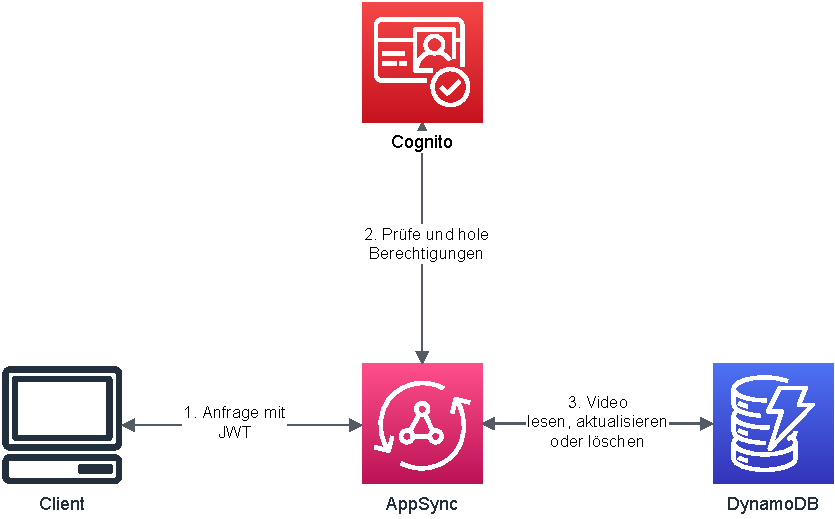
\includegraphics[width=0.75\columnwidth]{5_aws-amplify/laufzeitsicht_1.pdf}
  \caption{AWS Amplify - Laufzeitsicht - Lesen, Aktualisieren und Löschen eines Videos}
  \label{Amplify:laufzeitsicht1}
\end{figure}

\autoref{Amplify:laufzeitsicht1} stellt den Prozess dar, wie Videos von Nutzern gelesen, aktualisiert oder gelöscht werden. Dieser wird im folgenden Abschnitt näher erläutert:
\begin{enumerate}
  \item{Der Nutzer stellt eine Anfrage mittels GraphQL und dem JSON Webtoken.}
  \item{AppSync autorisiert den Nutzer und holt die Gruppenzugehörigkeit des Nutzers.}
  \item{Der Resolver leitet die Anfrage unter Berücksichtigung der Gruppenzugehörigkeit des Nutzers an DynamoDB weiter. Die nötigen Datenbankoperationen werden über DynamoDB ausgeführt.}
\end{enumerate}

Zusätzlich dazu müssen signierte temporäre Links erstellt werden, um die Sicherheit zu gewährleisten. Dieser Ablauf, der in \autoref{Amplify:laufzeitsicht2} dargestellt wird, enthält noch eine zusätzlich Abfrage auf S3, um den Link zu erstellen.

\begin{figure}
  \centering
  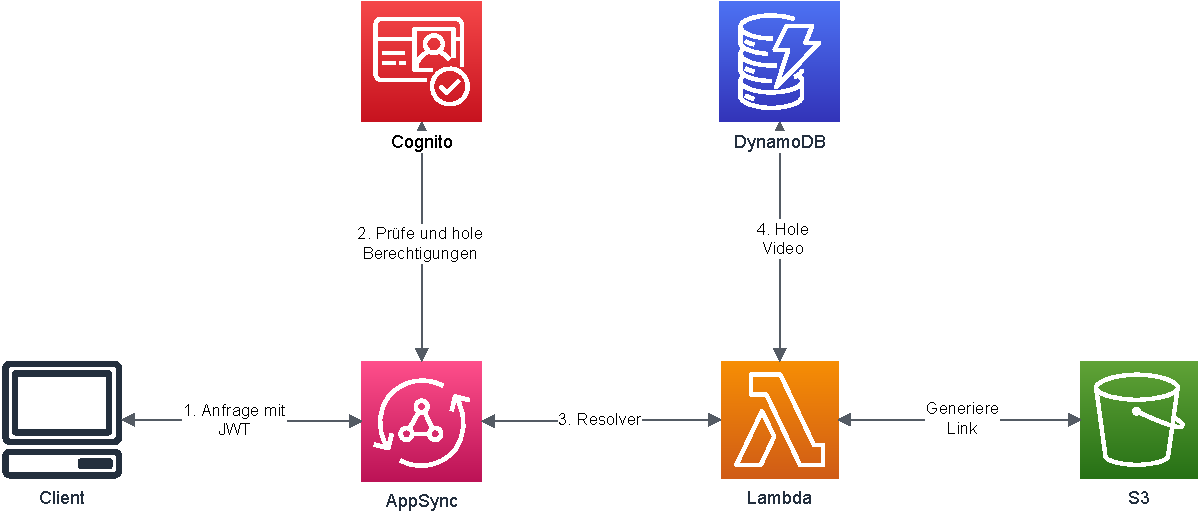
\includegraphics[width=1\columnwidth]{5_aws-amplify/laufzeitsicht_3.pdf}
  \caption{AWS Amplify - Laufzeitsicht - Erstellen von Links}
  \label{Amplify:laufzeitsicht2}
\end{figure}

\subsubsection{Erstellen eines Videos}

\autoref{Amplify:laufzeitsicht3} stellt den Prozess dar, wie ein Video erstellt wird.
\begin{enumerate}
  \item{Zunächst lädt der Nutzer das Video in den S3-Bucket hoch. Die Policy des S3-Buckets verwaltet den korrekten Zugriff auf die Ressource. Die hochgeladene Datei landet in einem privaten Ordner, der außerhalb des Backends ausschließlich für den Besitzer des Objekts aufrufbar ist. Das ist der Nutzer, der das Video hochgeladen hat.}
  \item{Erst dann erstellt der Nutzer eine Anfrage mittels GraphQL und dem JSON Webtoken.}
  \item{AppSync autorisiert den Nutzer und holt die Gruppenzugehörigkeit des Nutzers.}
  \item{Der Resolver führt die verknüpfte Lambda-Funktion aus.}
  \item{Die Funktion kopiert die hochgeladene Datei in einen weiteren Ordner, so dass der Besitzer diese nicht mehr verändern kann. Die hochgeladene Datei im Ursprungsordner wird daraufhin gelöscht.}
  \item{Die Funktion erstellt das Video in der DynamoDB-Tabelle.}
  \item{Die Funktion führt den MediaConvert-Job aus, um das Video mit dem Wasserzeichen zu versehen.}
  \item{Ist die Konvertierung abgeschlossen, benachrichtigt die EventBridge eine weitere Lambda-Funktion, welche das Video dann freischaltet.}
\end{enumerate}

\begin{figure}
  \centering
  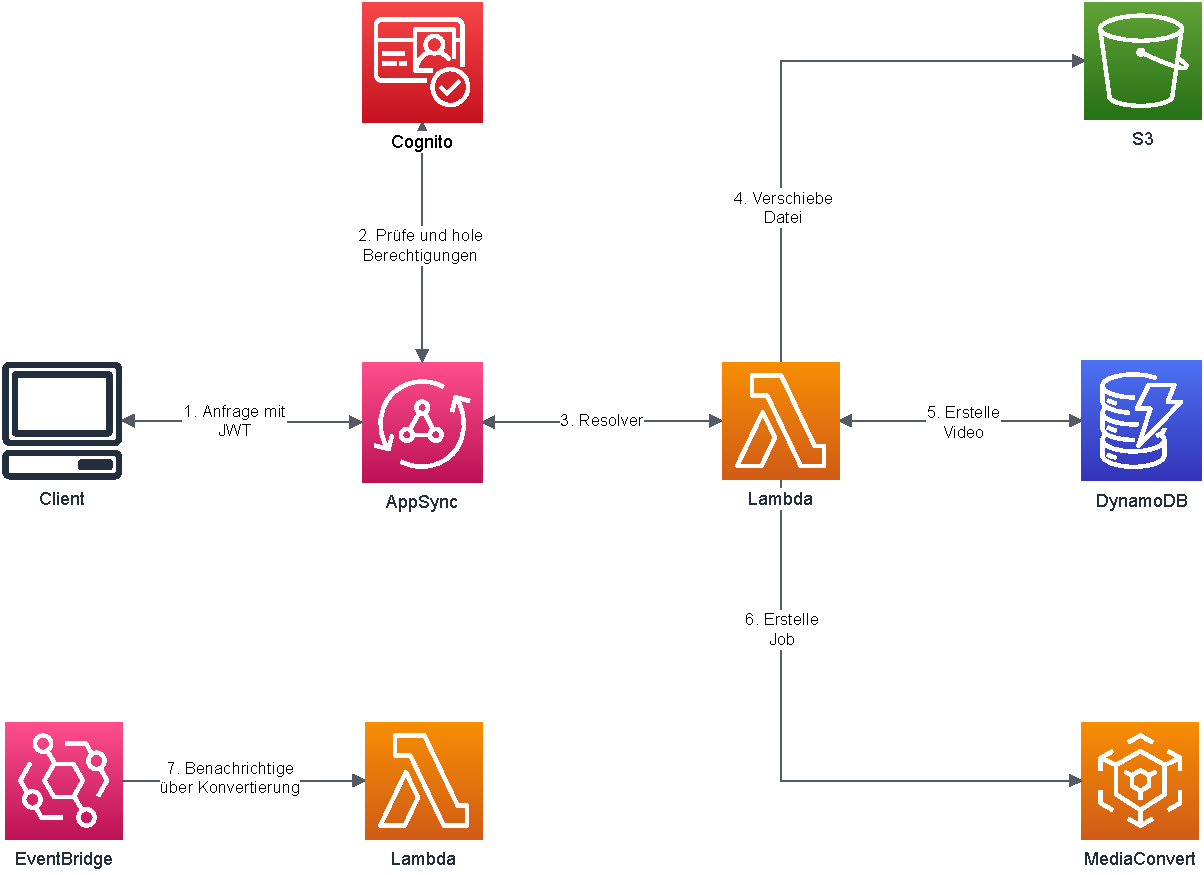
\includegraphics[width=1\columnwidth]{5_aws-amplify/laufzeitsicht_2.pdf}
  \caption{AWS Amplify - Laufzeitsicht - Erstellen eines Videos}
  \label{Amplify:laufzeitsicht3}
\end{figure}

\subsection{Verteilungssicht}

Die Verteilungssicht beschreibt, wie die Bausteine in \ac{AWS} über Stacks verteilt werden. Amplify bündelt die Verteilung des Backends und des Frontends über eine Pipeline. Diesen Sachverhalt stellt \autoref{Amplify:verteilungssicht} dar.

\begin{figure}
  \centering
  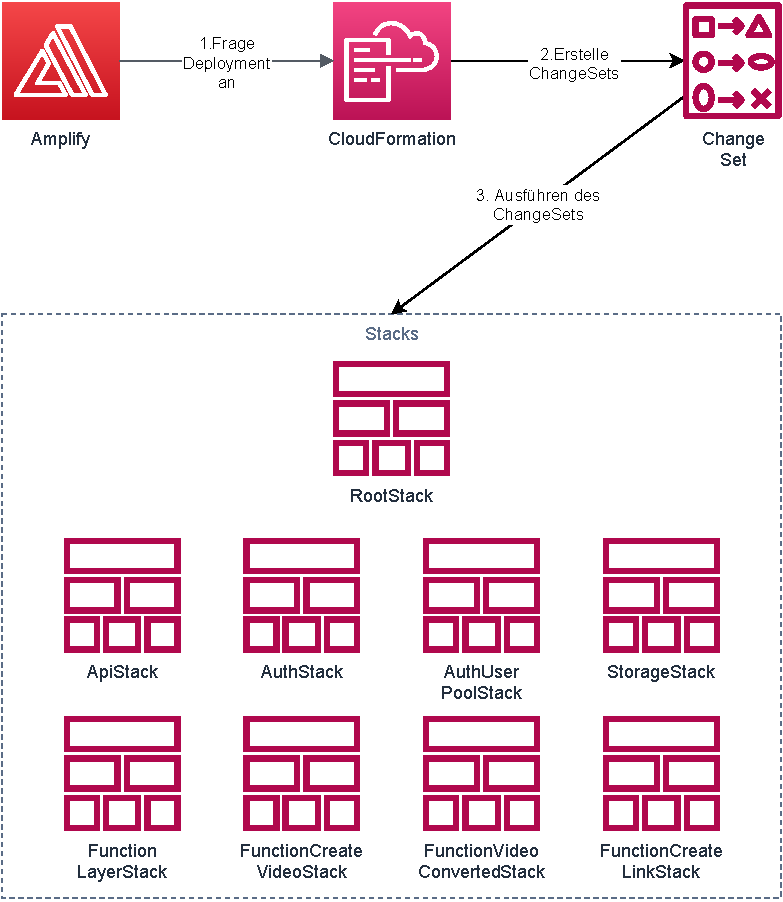
\includegraphics[width=0.75\columnwidth]{5_aws-amplify/verteilungssicht.pdf}
  \caption{AWS Amplify - Verteilungssicht}
  \label{Amplify:verteilungssicht}
\end{figure}

Amplify verteilt das Backend über die CloudFormation mittels Stacks. Außerdem werden nur Stacks und keine NestedStacks genutzt, was die Fehleranalyse vereinfacht. Um eine neue Änderung in das System einzuspielen, erzeugt die CloudFormation ein ChangeSet, welches die Differenz aus dem aktuellen Stand in der Cloud und dem gewünschten Zielzustand ist. Wenn beim Aktualisieren der Stacks ein Fehler auftritt, erfolgt ein Rollback.

Das Frontend wird separat, also nicht über Stacks, verteilt. Dazu nutzt Amplify einen gebündelten Dienst, der über die CloudFront läuft. Letzterer kann allerdings als Black-Box betrachtet werden, da der Entwickler diesen nur durch die Konfiguration beeinflussen kann.

\subsection{Querschnittliche Konzepte und Muster}

Logging
- CloudWatch

Backup
- AWS Backup

- Einbindung über \ac{AWS} Amplify:
  - AWS Elemental MediaConvert als extra Plugin
  - Anpassung an CF-Templates
- Permissions (IAM)

\subsection{Entwurfsentscheidungen}

\subsection{Risiken und technische Schulden}

- Auth: Anpassung, dass statt Identity ID die Pool User Id genutzt wird geht über https://github.com/aws-amplify/amplify-js/issues/54. Leider lässt sich das nicht persistieren, so dass man das bei jedem branch/Projekt neu eintragen muss. Wenn man es im CF-Template ändert, wird die Änderung beim Push rückgängig gemacht. Das ist nicht sehr flexibel. Ggf. Lösung finden und schauen, ob es doch geht.

- CDK als Alternative zu AWS Amplify, da es wesentlich flexibler

\section{Implementierung}
\section{Motivation}

Der Begriff des "`Software Engineering"' wurde erstmal 1968 auf einer Nato-Konferenz definiert \autocite{naur1969software}. Verglichen mit anderen Ingenieursdisiziplinen ist die Softwareentwicklung damit eine sehr junge Disziplin. Vorgehensweisen der Softwareentwicklung unterliegen dementsprechend einem stetigen Wandel.

Während Entwickler zu Beginn vor allem monolithische Architekturen entworfen haben, sind innerhalb kürzester Zeit weitere Architekturformen hinzugekommen. Neben der serviceorientierten Architektur spielen heute vor allem Architekturen basierend auf Microservices eine immer größer werdende Rolle. Auch das Deployment von Software ändert sich stetig. Während Entwickler zu Beginn Software auf einzelnen Servern ausgeliefert haben, ging der Trend über virtuelle Maschinen hin zu Container-Technologien wie Docker oder der Auslieferung von Software über Cloud-Dienste wie \ac{AWS} oder Google Cloud

Eines weiterer Trend in diesem Bereich ist die Nutzung von Backend-as-a-service-Tools wie \ac{AWS} Amplify oder Firebase \autocite{villamizar2017cost}.
\section{Zielsetzung und Methodik}

Das Ziel der Arbeit ist es die beiden Backend-as-a-service-Plattformen \ac{AWS} Amplify und Firebase zu vergleichen. Dies ist sinnvoll, um herauszufinden, welche der beiden Plattformen wirtschaftlich günstiger für die Entwicklung und das Hosting einer entsprechenden Software ist. Um dieses Ziel zu erreichen, muss definiert werden, anhand welcher Kriterien der Vergleich stattfindet. Die Arbeit fokussiert sich dabei auf den Entwicklungsaufwand sowie die monatlichen Kosten der Cloud. Um ein reales Beispiel zu simulieren, werden als nächstes die folgenden funktionalen (FA1 - FA7) und nicht-funktionalen (NF1 - NF6) Anforderungen sowie die Rahmenbedingungen (R1 - R5) für ein Video-Portal definiert. Dieses wird für diese Arbeit prototypisch entwickelt und ausgewertet.

\begin{description}
   \item[F1 - Registrierung] Das System muss dem Benutzer die Möglichkeit geben, sich zu registrieren. Dies erfolgt unter Angabe der Attribute E"=Mail, Telefonnummer und Passwort. \label{F1}
   \item[F2 - Login] Das System muss dem Benutzer die Möglichkeit geben, sich mit seiner E"=Mail Adresse und seinem Passwort einzuloggen. \label{F2}
   \item[F3 - Passwort vergessen] Das System muss dem Benutzer die Möglichkeit geben, sein Passwort durch eine Identitätsprüfung zu ändern. \label{F3}
   \item[F4 - Video hochladen] Das System muss dem Benutzer die Möglichkeit geben, ein neues Video zu erstellen. Dabei gibt der Benutzer die Attribute Titel, Beschreibung sowie die Videodatei im Format mp4 an. Das System muss das Video daraufhin automatisch mit einem Wasserzeichen versehen. Sobald dieser Prozess abgeschlossen ist, muss das System das Video freischalten, damit es beim Benutzer angezeigt wird. Ist der Prozess noch nicht abgeschlossen, soll dem Benutzer kein Video angezeigt werden. \label{F4}
   \item[F5 - Videos auflisten] Das System muss dem Benutzer die Möglichkeit geben, alle Videos aufzulisten. Die Videos müssen über das Titel"=Feld durchsuchbar sein. Dabei ist eine exakte Suche ausreichend. \label{F5}
   \item[F6 - Video bearbeiten] Das System muss dem Benutzer die Möglichkeit geben, eigene Videos zu bearbeiten, um den Titel oder die Beschreibung zu ändern. Trägt der Benutzer die Rolle des Administrators, darf dieser auch fremde Videos bearbeiten. \label{F6}
   \item[F7 - Videos löschen] Das System muss dem Benutzer die Möglichkeit geben, selbst hochgeladenen Videos zu löschen. Trägt der Nutzer die Rolle des Administrators, darf dieser auch fremde Videos löschen. \label{F7}
   \item[NF1 - Verfügbarkeit] Das System muss zu 99,9\% pro Jahr verfügbar sein. Ein Deployment darf nicht zu einem Systemausfall führen.\label{NF1}
   \item[NF2 - Skalierbarkeit] Das System muss bei Lastspitzen automatisch skalieren.\label{NF2}
   \item[NF3 - Analysierbarkeit] Das System muss so aufgesetzt werden, dass jeder Backend"=Aufruf durch Log"=Dateien nachvollziehbar ist.\label{NF3}
   \item[NF4 - Interoperabilität] Das System muss gängige Schnittstellen wie REST oder GraphQL anbieten.\label{NF4}
   \item[NF5 - Backups] Das System muss automatisiert Backups für mindestens sieben Tage anlegen.\label{NF6}
   \item[NF6 - Wiederherstellbarkeit] Das System muss im Falle eines Ausfalls oder eines Datenverlusts innerhalb von einer Stunde wiederherstellbar sein.\label{NF7}
   \item[R1 - Keine externen Cloud-Dienste] Das System darf nur Dienste innerhalb der zu entwickelnden Cloud nutzen. Beispielsweise dürfen keine externen Dienste für die Video"=Bearbeitung genutzt werden.
   \item[R2 - Keine Eigenentwicklungen] Das System sollte bei gängigen Problemen weitestgehend bestehende Lösungen der Cloud nutzen, statt Komponenten neu zu entwickeln. Beispielweise sollte eine User"=Authentifizierung nicht von Grund auf neu entwickelt werden. Wenn es keine bestehende Lösung gibt, darf die Software allerdings eine Eigenentwicklung nutzen.
   \item[R3 - Geringe Betriebskosten] Das System muss so konzipiert werden, dass die Betriebskosten der Anwendung minimal gehalten werden.
   \item[R4 - Backend"=Technologie] Das System soll im Backend Node.js, ferner JavaScript oder TypeScript, verwenden.
   \item[R5 - Frontend"=Technologie] Das System soll im Frontend React.js verwenden.
\end{description}
\section{Aufbau der Arbeit}

<todo> beschreibung der einzelnen Kapitel +

Diese Dokumentation orientiert sich an der Strukturvorlage arc42\autocite{starke2007strukturvorlage}. Zunächst wird dabei die Lösungsstrategie beschrieben. Diese gibt eine Übersicht über das Gesamtsystem. Darauf folgt die Dokumentation der drei Sichten. Die Bausteinsicht stellt dar, aus welchen Systembausteinen die Software besteht. Die Laufzeitsicht zeigt, wie die Systembausteine zur Laufzeit zusammenspielen. Die Verteilungssicht dokumentiert, wo die Komponenten liegen und wie sie verteilt werden. Anschließend werden querschnittliche Konzepte und Muster der Architektur präsentiert sowie wichtige Entwurfsentscheidungen dokumentiert. Zuletzt werden auch Risiken und technische Schulden dargestellt.

- weitestgehende keine Levels
- keine UML-Notation auf Grund von Cloud-Diensten
- keine Ausschreibung der Services, z.B. wird aus AWS Amplify ==> Amplify und aus Amazon Cognito ==> Cognito.
- In Grundlagen werden die Services jedoch einmal ausgeschrieben, dann nicht mehr.

\chapter{AWS Amplify}

Das folgende Kapitel beschreibt die Architektur und die Implementierung mit Amplify.

\section{Architektur}

todo

\subsection{Lösungsstrategie}

Die Architektur folgt dem Aufbau einer Drei"=Schichten"=Architektur:
\begin{itemize}
  \item Präsentationsschicht
    \begin{itemize}
      \item React.js
      \item amplify-js
    \end{itemize}
  \item Logikschicht
    \begin{itemize}
      \item AppSync
      \item Lambda
      \item Cognito
      \item Elemental MediaConvert
      \item EventBridge
      \item IAM
    \end{itemize}
  \item Datenhaltungsschicht
    \begin{itemize}
      \item DynamoDB
      \item S3
      \item Cognito
      \item IAM
      \item AWS Backup
    \end{itemize}
\end{itemize}

Die Dienste Cognito und IAM befindet sich zugleich in zwei Schichten, da dort neben der Logik für Authentifizierung und Autorisierung auch die Benutzer persistiert werden.

Durch die ausschließliche Verwendung interner Dienste von \ac{AWS}, keiner Eigenentwicklungen für die Benutzerverwaltung und den vorgegebenen Technologien sind die Rahmenbedingungen für dieses Projekt nicht missachtet, so dass die beiden Technologien weiterhin vergleichbar sind.

\autoref{Kap2:NFAs} zeigt Lösungsansätze, um die nichtfunktionalen Anforderungen, auch Qualitätsziele genannt, zu erreichen.

\begin{table}[h]
  \caption{Lösungsansatz für nichtfunktionale Anforderungen}
  \label{Kap2:NFAs}
  \renewcommand{\arraystretch}{1.2}
  \centering
  \sffamily
  \begin{footnotesize}
    \begin{tabularx}{0.9\textwidth}{l l X}
      \toprule
      \textbf{Anforderung} & \textbf{Dienst} & \textbf{Ansatz}\\
      \midrule
        \emph{Verfügbarkeit} & Amplify & Amplify bietet für Frontend und Backend ein Zero-Downtime Deployment. \\
        \emph{Skalierbarkeit} & - & Durch die Serverless-Architektur skalieren Dienste automatisch innerhalb der \ac{AWS}-Cloud.\\
        \emph{Analysierbarkeit} & CloudWatch & Durch den Einsatz von CloudWatch können Anfragen für jeden Dienst nachvollzogen werden.\\
        \emph{Interoperabilität} & AppSync & Durch den Einsatz von AppSync ist mit GraphQL eine einheitliche Schnittstelle sichergestellt.\\
        \emph{Backups} & AWS Backup & Durch den Einsatz von AWS Backup werden automatisiert Backups aufgesetzt.\\
        \emph{Wiederherstellbarkeit} & AWS Backup &  Das von AWS Backup erstellte Backup für die Datenbank DynamoDB kann manuell eingespielt werden.\\
      \bottomrule
    \end{tabularx}
  \end{footnotesize}
  \rmfamily
\end{table}

\subsection{Bausteinsicht}

Die Architektur ist unterteilt in Frontend (Präsentationsschicht) und Backend (Logik- und Datenhaltungsschicht). Das Frontend wird nicht näher beschrieben, da Amplify dieses vollständig verwaltet. Das Backend besteht aus Stacks, welche zugleich den Code als auch die Infrastruktur repräsentieren. Diese werden im folgenden Abschnitt dargestellt:
\begin{itemize}
  \item{Der \textit{RootStack} enthält alle darunterliegenden Stacks sowie Ressourcen zum Deployment von Amplify.}

  \item{Der \textit{ApiStack} besteht aus den Diensten AppSync und DynamoDB. AppSync besteht aus einer GraphQLApi, die ein GraphQLSchema enthält. Außerdem nutzt AppSync Resolver, um ein Mapping über VTL zur DynamoDB-Tabelle zu ermöglichen. Um eine Verbindung zu einer Lambda-Funktion zu ermöglichen, existiert auch mindestens eine DataSource.}

  \item{Der \textit{AuthStack} regelt die Authentifizierung und Autorisierung von Benutzern über den Dienst Cognito. Dieser besteht aus einem UserPool und einem IdentityPool und den entsprechenden IAM-Rollen und Policies. Des weiteren besteht der Stack aus einem UserPoolClient, über welchen Anfragen auf Cognito erfolgen können. Amplify definiert auch weitere Lambda-Funktionen, um zusätzliche Logik für die Authentifizierung zu ermöglichen.}

  \item{Der \textit{AuthUserPoolGroupStack} dient zur Verwaltung der zusätzlichen UserPoolGroup für Administratoren.}

  \item{Der \textit{StorageStack} dient zur Speicherung der Videos. Dieser enthält einen S3-Bucket sowie eine dazugehören Policy, welchen es Benutzern ermöglicht, Dateien in eigene Ordner hochzuladen sowie andere Ordner lesen zu dürfen. Die Policy unterscheidet zwischen öffentlichen, geschützten und privaten Geltungsbereichen.}

  \item{Der \textit{FunctionLayerStack} bündelt die Node.js-Module als Lambda-Layer, den die weiteren Lambda-Funktionen nutzen.}

  \item{Der \textit{FunctionCreateVideoStack} übernimmt die Erstellung eines Videos in Form einer Lambda-Funktion. Außerdem erstellt der Stack in MediaConvert ein JobTemplate und eine Queue. Des Weiteren definiert der Stack die nötige Policy und Rolle, um der Lambda-Funktion die Zugriffe auf andere Dienste zu ermöglichen.}

  \item{Der \textit{FunctionVideoConvertedStack} besteht aus einer EventBridge-Regel, die bei einer Konvertierung eines Videos aufgerufen wird. Außerdem wird eine Lambda-Funktion mit der nötigen Policy und Rolle erstellt.}

  \item{Der \textit{FunctionCreateLinkStack} besteht aus einer Lambda-Funktion und der nötigen Rolle und Policy, um einen signierten zeitlich begrenzt gültigen Video-Link zu erstellen.}
\end{itemize}

Die Stacks \textit{RootStack}, \textit{ApiStack}, \textit{AuthStack}, \textit{AuthUserPoolGroupStack} und \textit{StorageStack} erstellt Amplify selbst. Die restlichen Stacks sind selbst erstellte bzw. angepasste Plugins, da die Dienste nicht vollständig in Amplify vorhanden sind.

\subsection{Laufzeitsicht}

Die Laufzeitsicht beschreibt die wichtigsten Prozesse und wie die Bausteine miteinander interagieren.

\subsubsection{Lesen, Aktualisieren und Löschen eines Videos}

\begin{figure}
  \centering
  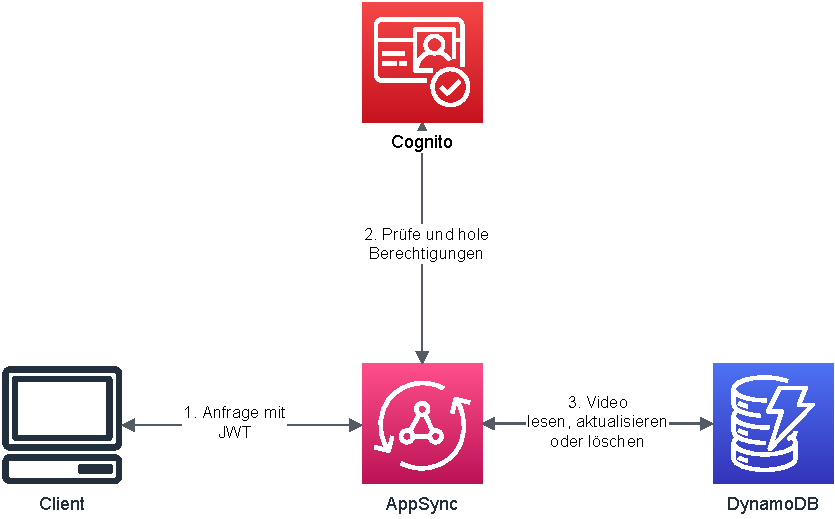
\includegraphics[width=0.75\columnwidth]{5_aws-amplify/laufzeitsicht_1.pdf}
  \caption{AWS Amplify - Laufzeitsicht - Lesen, Aktualisieren und Löschen eines Videos}
  \label{Amplify:laufzeitsicht1}
\end{figure}

\autoref{Amplify:laufzeitsicht1} stellt den Prozess dar, wie Videos von Nutzern gelesen, aktualisiert oder gelöscht werden. Dieser wird im folgenden Abschnitt näher erläutert:
\begin{enumerate}
  \item{Der Nutzer stellt eine Anfrage mittels GraphQL und dem JSON Webtoken.}
  \item{AppSync autorisiert den Nutzer und holt die Gruppenzugehörigkeit des Nutzers.}
  \item{Der Resolver leitet die Anfrage unter Berücksichtigung der Gruppenzugehörigkeit des Nutzers an DynamoDB weiter. Die nötigen Datenbankoperationen werden über DynamoDB ausgeführt.}
\end{enumerate}

Zusätzlich dazu müssen signierte temporäre Links erstellt werden, um die Sicherheit zu gewährleisten. Dieser Ablauf, der in \autoref{Amplify:laufzeitsicht2} dargestellt wird, enthält noch eine zusätzlich Abfrage auf S3, um den Link zu erstellen.

\begin{figure}
  \centering
  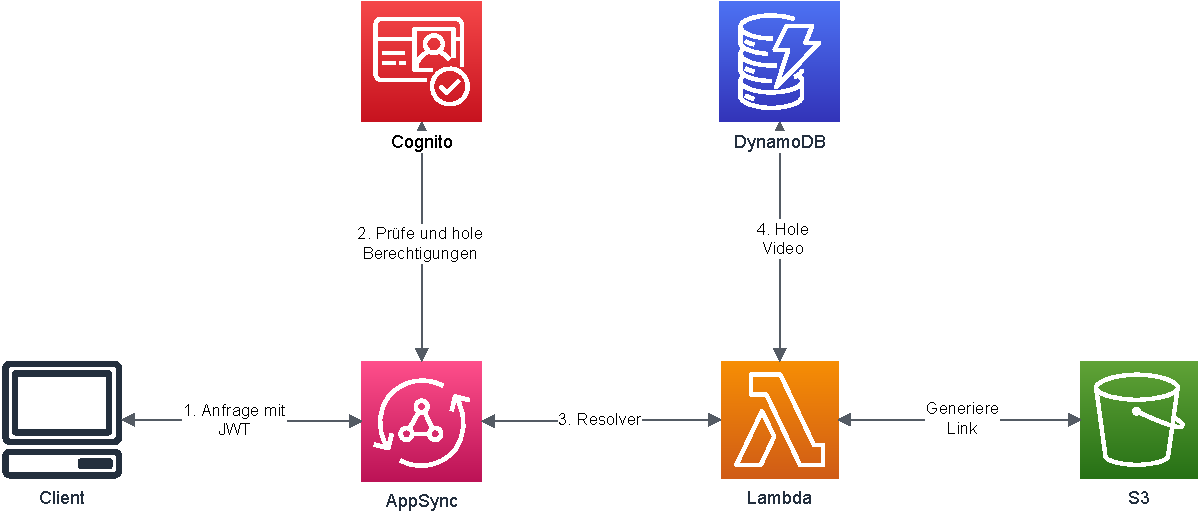
\includegraphics[width=1\columnwidth]{5_aws-amplify/laufzeitsicht_3.pdf}
  \caption{AWS Amplify - Laufzeitsicht - Erstellen von Links}
  \label{Amplify:laufzeitsicht2}
\end{figure}

\subsubsection{Erstellen eines Videos}

\autoref{Amplify:laufzeitsicht3} stellt den Prozess dar, wie ein Video erstellt wird.
\begin{enumerate}
  \item{Zunächst lädt der Nutzer das Video in den S3-Bucket hoch. Die Policy des S3-Buckets verwaltet den korrekten Zugriff auf die Ressource. Die hochgeladene Datei landet in einem privaten Ordner, der außerhalb des Backends ausschließlich für den Besitzer des Objekts aufrufbar ist. Das ist der Nutzer, der das Video hochgeladen hat.}
  \item{Erst dann erstellt der Nutzer eine Anfrage mittels GraphQL und dem JSON Webtoken.}
  \item{AppSync autorisiert den Nutzer und holt die Gruppenzugehörigkeit des Nutzers.}
  \item{Der Resolver führt die verknüpfte Lambda-Funktion aus.}
  \item{Die Funktion kopiert die hochgeladene Datei in einen weiteren Ordner, so dass der Besitzer diese nicht mehr verändern kann. Die hochgeladene Datei im Ursprungsordner wird daraufhin gelöscht.}
  \item{Die Funktion erstellt das Video in der DynamoDB-Tabelle.}
  \item{Die Funktion führt den MediaConvert-Job aus, um das Video mit dem Wasserzeichen zu versehen.}
  \item{Ist die Konvertierung abgeschlossen, benachrichtigt die EventBridge eine weitere Lambda-Funktion, welche das Video dann freischaltet.}
\end{enumerate}

\begin{figure}
  \centering
  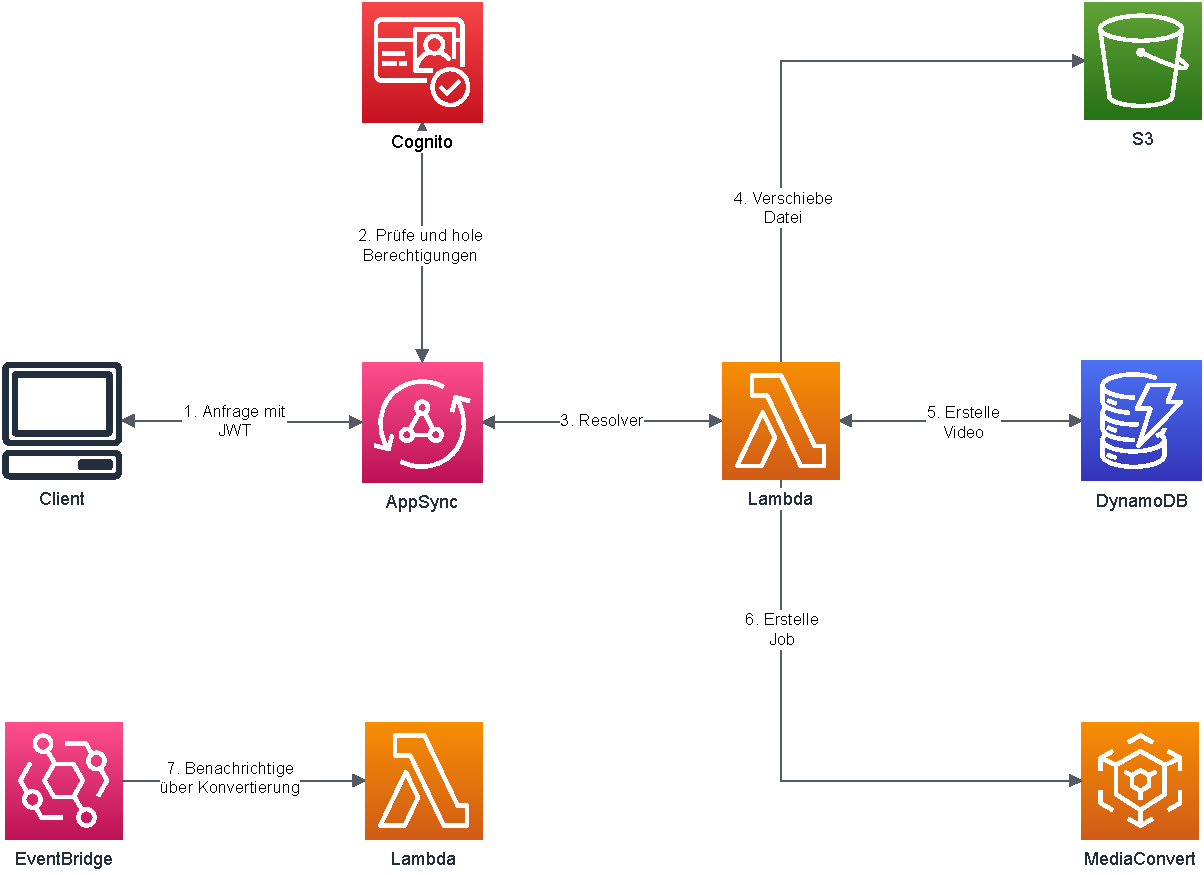
\includegraphics[width=1\columnwidth]{5_aws-amplify/laufzeitsicht_2.pdf}
  \caption{AWS Amplify - Laufzeitsicht - Erstellen eines Videos}
  \label{Amplify:laufzeitsicht3}
\end{figure}

\subsection{Verteilungssicht}

Die Verteilungssicht beschreibt, wie die Bausteine in \ac{AWS} über Stacks verteilt werden. Amplify bündelt die Verteilung des Backends und des Frontends über eine Pipeline. Diesen Sachverhalt stellt \autoref{Amplify:verteilungssicht} dar.

\begin{figure}
  \centering
  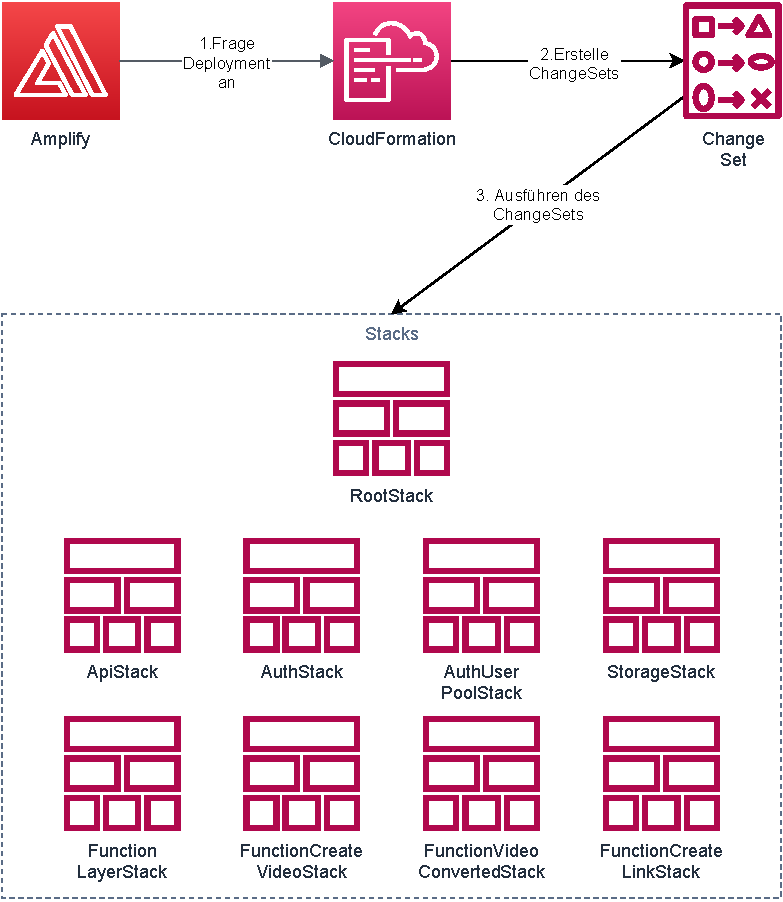
\includegraphics[width=0.75\columnwidth]{5_aws-amplify/verteilungssicht.pdf}
  \caption{AWS Amplify - Verteilungssicht}
  \label{Amplify:verteilungssicht}
\end{figure}

Amplify verteilt das Backend über die CloudFormation mittels Stacks. Außerdem werden nur Stacks und keine NestedStacks genutzt, was die Fehleranalyse vereinfacht. Um eine neue Änderung in das System einzuspielen, erzeugt die CloudFormation ein ChangeSet, welches die Differenz aus dem aktuellen Stand in der Cloud und dem gewünschten Zielzustand ist. Wenn beim Aktualisieren der Stacks ein Fehler auftritt, erfolgt ein Rollback.

Das Frontend wird separat, also nicht über Stacks, verteilt. Dazu nutzt Amplify einen gebündelten Dienst, der über die CloudFront läuft. Letzterer kann allerdings als Black-Box betrachtet werden, da der Entwickler diesen nur durch die Konfiguration beeinflussen kann.

\subsection{Querschnittliche Konzepte und Muster}

Logging
- CloudWatch

Backup
- AWS Backup

- Einbindung über \ac{AWS} Amplify:
  - AWS Elemental MediaConvert als extra Plugin
  - Anpassung an CF-Templates
- Permissions (IAM)

\subsection{Entwurfsentscheidungen}

\subsection{Risiken und technische Schulden}

- Auth: Anpassung, dass statt Identity ID die Pool User Id genutzt wird geht über https://github.com/aws-amplify/amplify-js/issues/54. Leider lässt sich das nicht persistieren, so dass man das bei jedem branch/Projekt neu eintragen muss. Wenn man es im CF-Template ändert, wird die Änderung beim Push rückgängig gemacht. Das ist nicht sehr flexibel. Ggf. Lösung finden und schauen, ob es doch geht.

- CDK als Alternative zu AWS Amplify, da es wesentlich flexibler

\section{Implementierung}

\chapter{AWS Amplify}

Das folgende Kapitel beschreibt die Architektur und die Implementierung mit Amplify.

\section{Architektur}

todo

\subsection{Lösungsstrategie}

Die Architektur folgt dem Aufbau einer Drei"=Schichten"=Architektur:
\begin{itemize}
  \item Präsentationsschicht
    \begin{itemize}
      \item React.js
      \item amplify-js
    \end{itemize}
  \item Logikschicht
    \begin{itemize}
      \item AppSync
      \item Lambda
      \item Cognito
      \item Elemental MediaConvert
      \item EventBridge
      \item IAM
    \end{itemize}
  \item Datenhaltungsschicht
    \begin{itemize}
      \item DynamoDB
      \item S3
      \item Cognito
      \item IAM
      \item AWS Backup
    \end{itemize}
\end{itemize}

Die Dienste Cognito und IAM befindet sich zugleich in zwei Schichten, da dort neben der Logik für Authentifizierung und Autorisierung auch die Benutzer persistiert werden.

Durch die ausschließliche Verwendung interner Dienste von \ac{AWS}, keiner Eigenentwicklungen für die Benutzerverwaltung und den vorgegebenen Technologien sind die Rahmenbedingungen für dieses Projekt nicht missachtet, so dass die beiden Technologien weiterhin vergleichbar sind.

\autoref{Kap2:NFAs} zeigt Lösungsansätze, um die nichtfunktionalen Anforderungen, auch Qualitätsziele genannt, zu erreichen.

\begin{table}[h]
  \caption{Lösungsansatz für nichtfunktionale Anforderungen}
  \label{Kap2:NFAs}
  \renewcommand{\arraystretch}{1.2}
  \centering
  \sffamily
  \begin{footnotesize}
    \begin{tabularx}{0.9\textwidth}{l l X}
      \toprule
      \textbf{Anforderung} & \textbf{Dienst} & \textbf{Ansatz}\\
      \midrule
        \emph{Verfügbarkeit} & Amplify & Amplify bietet für Frontend und Backend ein Zero-Downtime Deployment. \\
        \emph{Skalierbarkeit} & - & Durch die Serverless-Architektur skalieren Dienste automatisch innerhalb der \ac{AWS}-Cloud.\\
        \emph{Analysierbarkeit} & CloudWatch & Durch den Einsatz von CloudWatch können Anfragen für jeden Dienst nachvollzogen werden.\\
        \emph{Interoperabilität} & AppSync & Durch den Einsatz von AppSync ist mit GraphQL eine einheitliche Schnittstelle sichergestellt.\\
        \emph{Backups} & AWS Backup & Durch den Einsatz von AWS Backup werden automatisiert Backups aufgesetzt.\\
        \emph{Wiederherstellbarkeit} & AWS Backup &  Das von AWS Backup erstellte Backup für die Datenbank DynamoDB kann manuell eingespielt werden.\\
      \bottomrule
    \end{tabularx}
  \end{footnotesize}
  \rmfamily
\end{table}

\subsection{Bausteinsicht}

Die Architektur ist unterteilt in Frontend (Präsentationsschicht) und Backend (Logik- und Datenhaltungsschicht). Das Frontend wird nicht näher beschrieben, da Amplify dieses vollständig verwaltet. Das Backend besteht aus Stacks, welche zugleich den Code als auch die Infrastruktur repräsentieren. Diese werden im folgenden Abschnitt dargestellt:
\begin{itemize}
  \item{Der \textit{RootStack} enthält alle darunterliegenden Stacks sowie Ressourcen zum Deployment von Amplify.}

  \item{Der \textit{ApiStack} besteht aus den Diensten AppSync und DynamoDB. AppSync besteht aus einer GraphQLApi, die ein GraphQLSchema enthält. Außerdem nutzt AppSync Resolver, um ein Mapping über VTL zur DynamoDB-Tabelle zu ermöglichen. Um eine Verbindung zu einer Lambda-Funktion zu ermöglichen, existiert auch mindestens eine DataSource.}

  \item{Der \textit{AuthStack} regelt die Authentifizierung und Autorisierung von Benutzern über den Dienst Cognito. Dieser besteht aus einem UserPool und einem IdentityPool und den entsprechenden IAM-Rollen und Policies. Des weiteren besteht der Stack aus einem UserPoolClient, über welchen Anfragen auf Cognito erfolgen können. Amplify definiert auch weitere Lambda-Funktionen, um zusätzliche Logik für die Authentifizierung zu ermöglichen.}

  \item{Der \textit{AuthUserPoolGroupStack} dient zur Verwaltung der zusätzlichen UserPoolGroup für Administratoren.}

  \item{Der \textit{StorageStack} dient zur Speicherung der Videos. Dieser enthält einen S3-Bucket sowie eine dazugehören Policy, welchen es Benutzern ermöglicht, Dateien in eigene Ordner hochzuladen sowie andere Ordner lesen zu dürfen. Die Policy unterscheidet zwischen öffentlichen, geschützten und privaten Geltungsbereichen.}

  \item{Der \textit{FunctionLayerStack} bündelt die Node.js-Module als Lambda-Layer, den die weiteren Lambda-Funktionen nutzen.}

  \item{Der \textit{FunctionCreateVideoStack} übernimmt die Erstellung eines Videos in Form einer Lambda-Funktion. Außerdem erstellt der Stack in MediaConvert ein JobTemplate und eine Queue. Des Weiteren definiert der Stack die nötige Policy und Rolle, um der Lambda-Funktion die Zugriffe auf andere Dienste zu ermöglichen.}

  \item{Der \textit{FunctionVideoConvertedStack} besteht aus einer EventBridge-Regel, die bei einer Konvertierung eines Videos aufgerufen wird. Außerdem wird eine Lambda-Funktion mit der nötigen Policy und Rolle erstellt.}

  \item{Der \textit{FunctionCreateLinkStack} besteht aus einer Lambda-Funktion und der nötigen Rolle und Policy, um einen signierten zeitlich begrenzt gültigen Video-Link zu erstellen.}
\end{itemize}

Die Stacks \textit{RootStack}, \textit{ApiStack}, \textit{AuthStack}, \textit{AuthUserPoolGroupStack} und \textit{StorageStack} erstellt Amplify selbst. Die restlichen Stacks sind selbst erstellte bzw. angepasste Plugins, da die Dienste nicht vollständig in Amplify vorhanden sind.

\subsection{Laufzeitsicht}

Die Laufzeitsicht beschreibt die wichtigsten Prozesse und wie die Bausteine miteinander interagieren.

\subsubsection{Lesen, Aktualisieren und Löschen eines Videos}

\begin{figure}
  \centering
  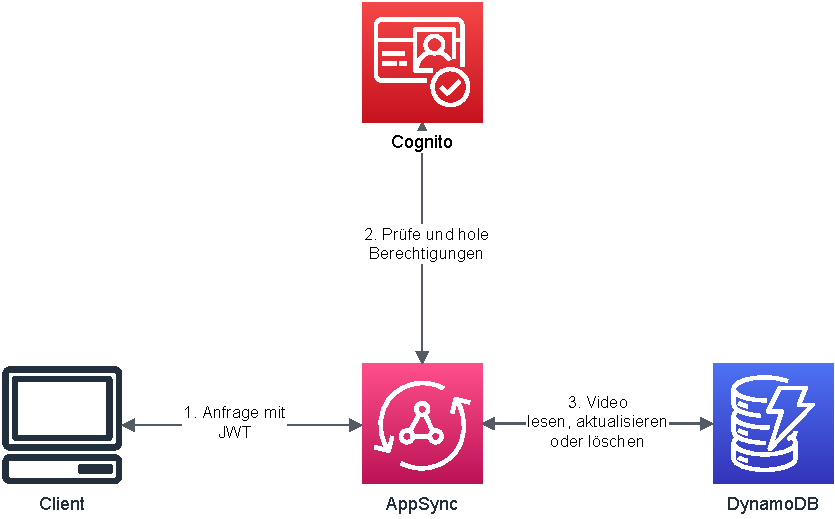
\includegraphics[width=0.75\columnwidth]{5_aws-amplify/laufzeitsicht_1.pdf}
  \caption{AWS Amplify - Laufzeitsicht - Lesen, Aktualisieren und Löschen eines Videos}
  \label{Amplify:laufzeitsicht1}
\end{figure}

\autoref{Amplify:laufzeitsicht1} stellt den Prozess dar, wie Videos von Nutzern gelesen, aktualisiert oder gelöscht werden. Dieser wird im folgenden Abschnitt näher erläutert:
\begin{enumerate}
  \item{Der Nutzer stellt eine Anfrage mittels GraphQL und dem JSON Webtoken.}
  \item{AppSync autorisiert den Nutzer und holt die Gruppenzugehörigkeit des Nutzers.}
  \item{Der Resolver leitet die Anfrage unter Berücksichtigung der Gruppenzugehörigkeit des Nutzers an DynamoDB weiter. Die nötigen Datenbankoperationen werden über DynamoDB ausgeführt.}
\end{enumerate}

Zusätzlich dazu müssen signierte temporäre Links erstellt werden, um die Sicherheit zu gewährleisten. Dieser Ablauf, der in \autoref{Amplify:laufzeitsicht2} dargestellt wird, enthält noch eine zusätzlich Abfrage auf S3, um den Link zu erstellen.

\begin{figure}
  \centering
  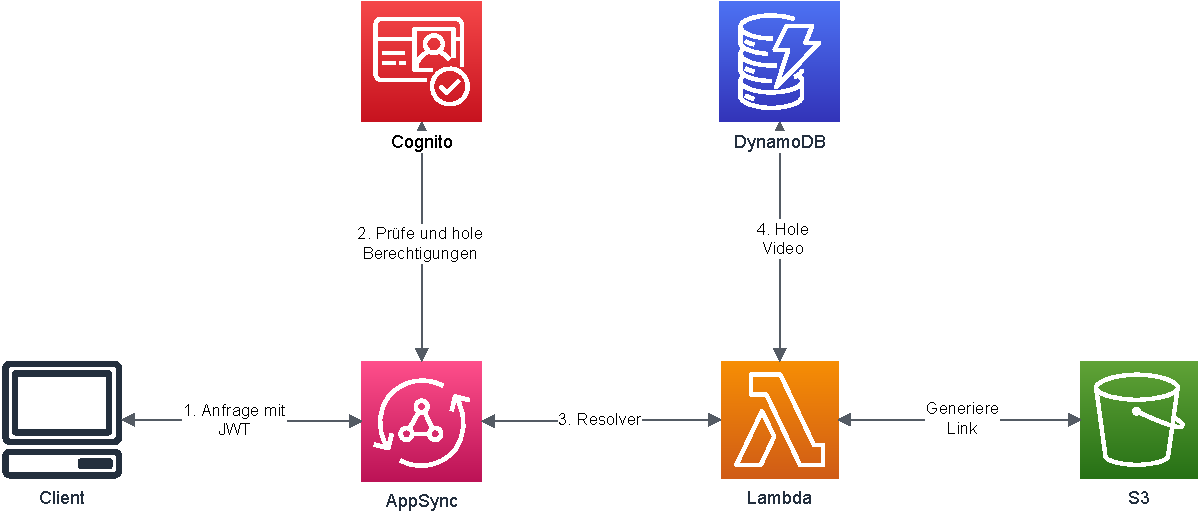
\includegraphics[width=1\columnwidth]{5_aws-amplify/laufzeitsicht_3.pdf}
  \caption{AWS Amplify - Laufzeitsicht - Erstellen von Links}
  \label{Amplify:laufzeitsicht2}
\end{figure}

\subsubsection{Erstellen eines Videos}

\autoref{Amplify:laufzeitsicht3} stellt den Prozess dar, wie ein Video erstellt wird.
\begin{enumerate}
  \item{Zunächst lädt der Nutzer das Video in den S3-Bucket hoch. Die Policy des S3-Buckets verwaltet den korrekten Zugriff auf die Ressource. Die hochgeladene Datei landet in einem privaten Ordner, der außerhalb des Backends ausschließlich für den Besitzer des Objekts aufrufbar ist. Das ist der Nutzer, der das Video hochgeladen hat.}
  \item{Erst dann erstellt der Nutzer eine Anfrage mittels GraphQL und dem JSON Webtoken.}
  \item{AppSync autorisiert den Nutzer und holt die Gruppenzugehörigkeit des Nutzers.}
  \item{Der Resolver führt die verknüpfte Lambda-Funktion aus.}
  \item{Die Funktion kopiert die hochgeladene Datei in einen weiteren Ordner, so dass der Besitzer diese nicht mehr verändern kann. Die hochgeladene Datei im Ursprungsordner wird daraufhin gelöscht.}
  \item{Die Funktion erstellt das Video in der DynamoDB-Tabelle.}
  \item{Die Funktion führt den MediaConvert-Job aus, um das Video mit dem Wasserzeichen zu versehen.}
  \item{Ist die Konvertierung abgeschlossen, benachrichtigt die EventBridge eine weitere Lambda-Funktion, welche das Video dann freischaltet.}
\end{enumerate}

\begin{figure}
  \centering
  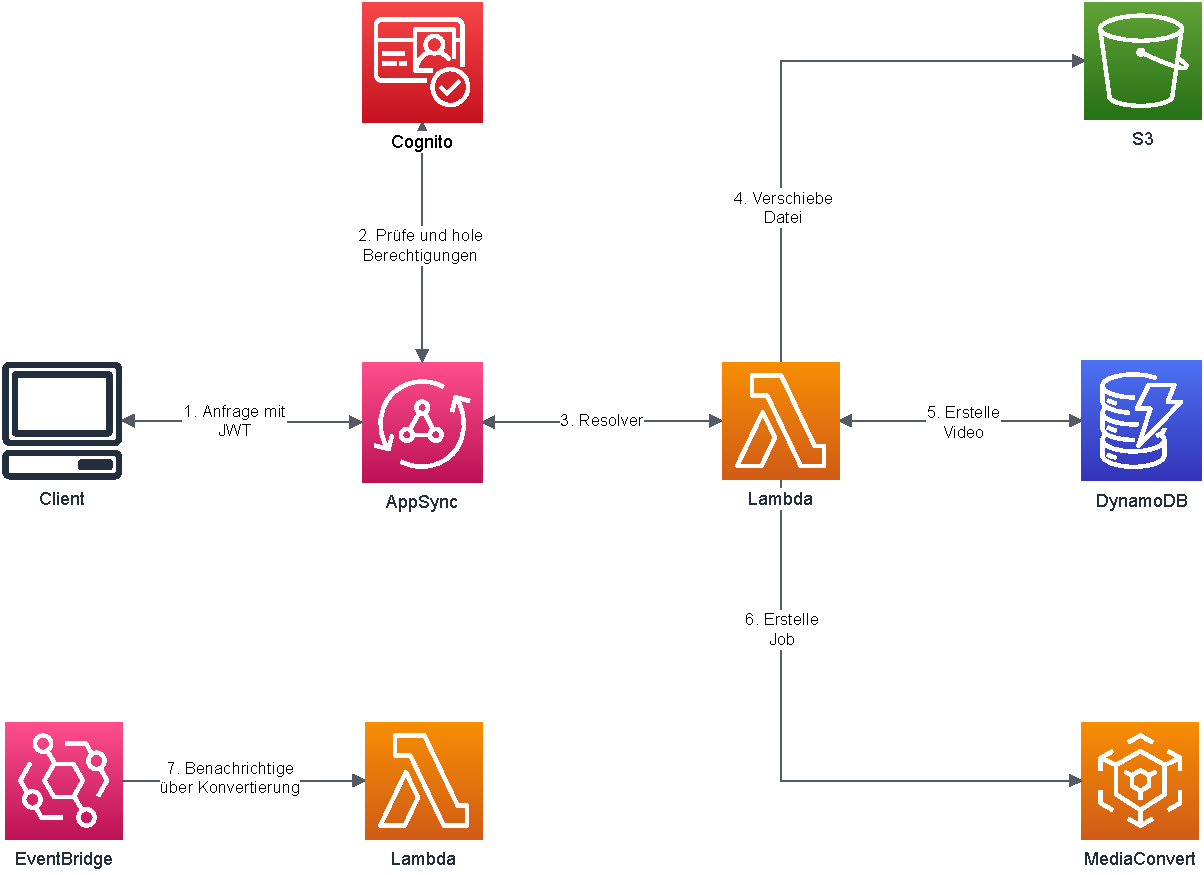
\includegraphics[width=1\columnwidth]{5_aws-amplify/laufzeitsicht_2.pdf}
  \caption{AWS Amplify - Laufzeitsicht - Erstellen eines Videos}
  \label{Amplify:laufzeitsicht3}
\end{figure}

\subsection{Verteilungssicht}

Die Verteilungssicht beschreibt, wie die Bausteine in \ac{AWS} über Stacks verteilt werden. Amplify bündelt die Verteilung des Backends und des Frontends über eine Pipeline. Diesen Sachverhalt stellt \autoref{Amplify:verteilungssicht} dar.

\begin{figure}
  \centering
  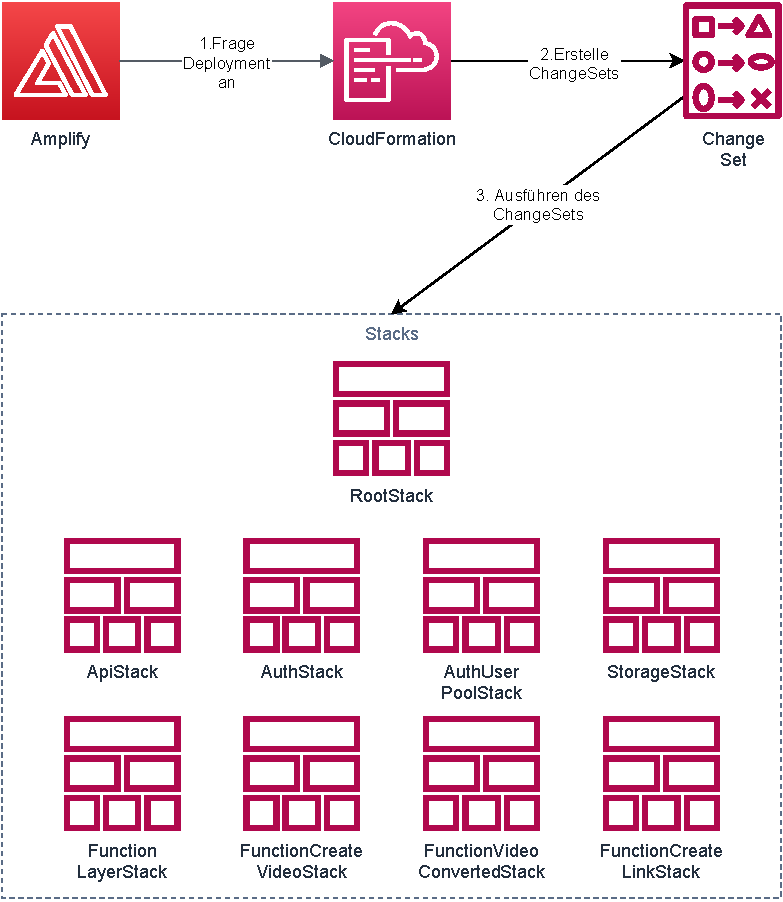
\includegraphics[width=0.75\columnwidth]{5_aws-amplify/verteilungssicht.pdf}
  \caption{AWS Amplify - Verteilungssicht}
  \label{Amplify:verteilungssicht}
\end{figure}

Amplify verteilt das Backend über die CloudFormation mittels Stacks. Außerdem werden nur Stacks und keine NestedStacks genutzt, was die Fehleranalyse vereinfacht. Um eine neue Änderung in das System einzuspielen, erzeugt die CloudFormation ein ChangeSet, welches die Differenz aus dem aktuellen Stand in der Cloud und dem gewünschten Zielzustand ist. Wenn beim Aktualisieren der Stacks ein Fehler auftritt, erfolgt ein Rollback.

Das Frontend wird separat, also nicht über Stacks, verteilt. Dazu nutzt Amplify einen gebündelten Dienst, der über die CloudFront läuft. Letzterer kann allerdings als Black-Box betrachtet werden, da der Entwickler diesen nur durch die Konfiguration beeinflussen kann.

\subsection{Querschnittliche Konzepte und Muster}

Logging
- CloudWatch

Backup
- AWS Backup

- Einbindung über \ac{AWS} Amplify:
  - AWS Elemental MediaConvert als extra Plugin
  - Anpassung an CF-Templates
- Permissions (IAM)

\subsection{Entwurfsentscheidungen}

\subsection{Risiken und technische Schulden}

- Auth: Anpassung, dass statt Identity ID die Pool User Id genutzt wird geht über https://github.com/aws-amplify/amplify-js/issues/54. Leider lässt sich das nicht persistieren, so dass man das bei jedem branch/Projekt neu eintragen muss. Wenn man es im CF-Template ändert, wird die Änderung beim Push rückgängig gemacht. Das ist nicht sehr flexibel. Ggf. Lösung finden und schauen, ob es doch geht.

- CDK als Alternative zu AWS Amplify, da es wesentlich flexibler

\section{Implementierung}

\chapter{AWS Amplify}

Das folgende Kapitel beschreibt die Architektur und die Implementierung mit Amplify.

\section{Architektur}

todo

\subsection{Lösungsstrategie}

Die Architektur folgt dem Aufbau einer Drei"=Schichten"=Architektur:
\begin{itemize}
  \item Präsentationsschicht
    \begin{itemize}
      \item React.js
      \item amplify-js
    \end{itemize}
  \item Logikschicht
    \begin{itemize}
      \item AppSync
      \item Lambda
      \item Cognito
      \item Elemental MediaConvert
      \item EventBridge
      \item IAM
    \end{itemize}
  \item Datenhaltungsschicht
    \begin{itemize}
      \item DynamoDB
      \item S3
      \item Cognito
      \item IAM
      \item AWS Backup
    \end{itemize}
\end{itemize}

Die Dienste Cognito und IAM befindet sich zugleich in zwei Schichten, da dort neben der Logik für Authentifizierung und Autorisierung auch die Benutzer persistiert werden.

Durch die ausschließliche Verwendung interner Dienste von \ac{AWS}, keiner Eigenentwicklungen für die Benutzerverwaltung und den vorgegebenen Technologien sind die Rahmenbedingungen für dieses Projekt nicht missachtet, so dass die beiden Technologien weiterhin vergleichbar sind.

\autoref{Kap2:NFAs} zeigt Lösungsansätze, um die nichtfunktionalen Anforderungen, auch Qualitätsziele genannt, zu erreichen.

\begin{table}[h]
  \caption{Lösungsansatz für nichtfunktionale Anforderungen}
  \label{Kap2:NFAs}
  \renewcommand{\arraystretch}{1.2}
  \centering
  \sffamily
  \begin{footnotesize}
    \begin{tabularx}{0.9\textwidth}{l l X}
      \toprule
      \textbf{Anforderung} & \textbf{Dienst} & \textbf{Ansatz}\\
      \midrule
        \emph{Verfügbarkeit} & Amplify & Amplify bietet für Frontend und Backend ein Zero-Downtime Deployment. \\
        \emph{Skalierbarkeit} & - & Durch die Serverless-Architektur skalieren Dienste automatisch innerhalb der \ac{AWS}-Cloud.\\
        \emph{Analysierbarkeit} & CloudWatch & Durch den Einsatz von CloudWatch können Anfragen für jeden Dienst nachvollzogen werden.\\
        \emph{Interoperabilität} & AppSync & Durch den Einsatz von AppSync ist mit GraphQL eine einheitliche Schnittstelle sichergestellt.\\
        \emph{Backups} & AWS Backup & Durch den Einsatz von AWS Backup werden automatisiert Backups aufgesetzt.\\
        \emph{Wiederherstellbarkeit} & AWS Backup &  Das von AWS Backup erstellte Backup für die Datenbank DynamoDB kann manuell eingespielt werden.\\
      \bottomrule
    \end{tabularx}
  \end{footnotesize}
  \rmfamily
\end{table}

\subsection{Bausteinsicht}

Die Architektur ist unterteilt in Frontend (Präsentationsschicht) und Backend (Logik- und Datenhaltungsschicht). Das Frontend wird nicht näher beschrieben, da Amplify dieses vollständig verwaltet. Das Backend besteht aus Stacks, welche zugleich den Code als auch die Infrastruktur repräsentieren. Diese werden im folgenden Abschnitt dargestellt:
\begin{itemize}
  \item{Der \textit{RootStack} enthält alle darunterliegenden Stacks sowie Ressourcen zum Deployment von Amplify.}

  \item{Der \textit{ApiStack} besteht aus den Diensten AppSync und DynamoDB. AppSync besteht aus einer GraphQLApi, die ein GraphQLSchema enthält. Außerdem nutzt AppSync Resolver, um ein Mapping über VTL zur DynamoDB-Tabelle zu ermöglichen. Um eine Verbindung zu einer Lambda-Funktion zu ermöglichen, existiert auch mindestens eine DataSource.}

  \item{Der \textit{AuthStack} regelt die Authentifizierung und Autorisierung von Benutzern über den Dienst Cognito. Dieser besteht aus einem UserPool und einem IdentityPool und den entsprechenden IAM-Rollen und Policies. Des weiteren besteht der Stack aus einem UserPoolClient, über welchen Anfragen auf Cognito erfolgen können. Amplify definiert auch weitere Lambda-Funktionen, um zusätzliche Logik für die Authentifizierung zu ermöglichen.}

  \item{Der \textit{AuthUserPoolGroupStack} dient zur Verwaltung der zusätzlichen UserPoolGroup für Administratoren.}

  \item{Der \textit{StorageStack} dient zur Speicherung der Videos. Dieser enthält einen S3-Bucket sowie eine dazugehören Policy, welchen es Benutzern ermöglicht, Dateien in eigene Ordner hochzuladen sowie andere Ordner lesen zu dürfen. Die Policy unterscheidet zwischen öffentlichen, geschützten und privaten Geltungsbereichen.}

  \item{Der \textit{FunctionLayerStack} bündelt die Node.js-Module als Lambda-Layer, den die weiteren Lambda-Funktionen nutzen.}

  \item{Der \textit{FunctionCreateVideoStack} übernimmt die Erstellung eines Videos in Form einer Lambda-Funktion. Außerdem erstellt der Stack in MediaConvert ein JobTemplate und eine Queue. Des Weiteren definiert der Stack die nötige Policy und Rolle, um der Lambda-Funktion die Zugriffe auf andere Dienste zu ermöglichen.}

  \item{Der \textit{FunctionVideoConvertedStack} besteht aus einer EventBridge-Regel, die bei einer Konvertierung eines Videos aufgerufen wird. Außerdem wird eine Lambda-Funktion mit der nötigen Policy und Rolle erstellt.}

  \item{Der \textit{FunctionCreateLinkStack} besteht aus einer Lambda-Funktion und der nötigen Rolle und Policy, um einen signierten zeitlich begrenzt gültigen Video-Link zu erstellen.}
\end{itemize}

Die Stacks \textit{RootStack}, \textit{ApiStack}, \textit{AuthStack}, \textit{AuthUserPoolGroupStack} und \textit{StorageStack} erstellt Amplify selbst. Die restlichen Stacks sind selbst erstellte bzw. angepasste Plugins, da die Dienste nicht vollständig in Amplify vorhanden sind.

\subsection{Laufzeitsicht}

Die Laufzeitsicht beschreibt die wichtigsten Prozesse und wie die Bausteine miteinander interagieren.

\subsubsection{Lesen, Aktualisieren und Löschen eines Videos}

\begin{figure}
  \centering
  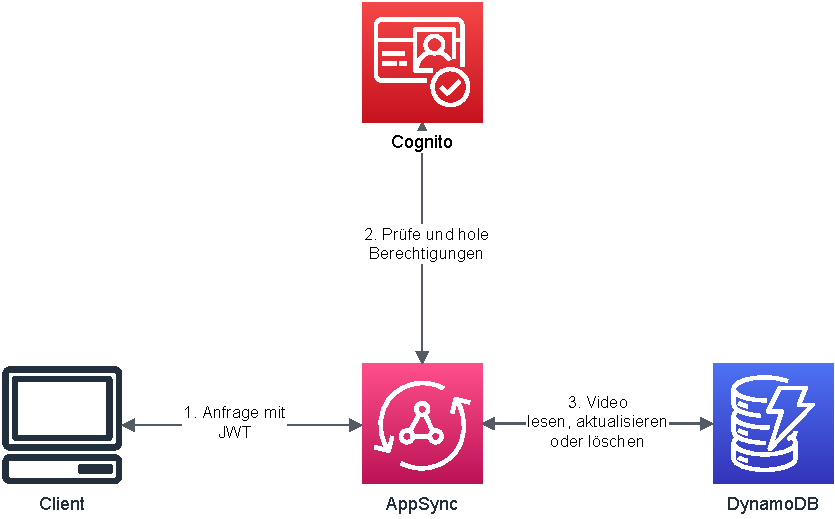
\includegraphics[width=0.75\columnwidth]{5_aws-amplify/laufzeitsicht_1.pdf}
  \caption{AWS Amplify - Laufzeitsicht - Lesen, Aktualisieren und Löschen eines Videos}
  \label{Amplify:laufzeitsicht1}
\end{figure}

\autoref{Amplify:laufzeitsicht1} stellt den Prozess dar, wie Videos von Nutzern gelesen, aktualisiert oder gelöscht werden. Dieser wird im folgenden Abschnitt näher erläutert:
\begin{enumerate}
  \item{Der Nutzer stellt eine Anfrage mittels GraphQL und dem JSON Webtoken.}
  \item{AppSync autorisiert den Nutzer und holt die Gruppenzugehörigkeit des Nutzers.}
  \item{Der Resolver leitet die Anfrage unter Berücksichtigung der Gruppenzugehörigkeit des Nutzers an DynamoDB weiter. Die nötigen Datenbankoperationen werden über DynamoDB ausgeführt.}
\end{enumerate}

Zusätzlich dazu müssen signierte temporäre Links erstellt werden, um die Sicherheit zu gewährleisten. Dieser Ablauf, der in \autoref{Amplify:laufzeitsicht2} dargestellt wird, enthält noch eine zusätzlich Abfrage auf S3, um den Link zu erstellen.

\begin{figure}
  \centering
  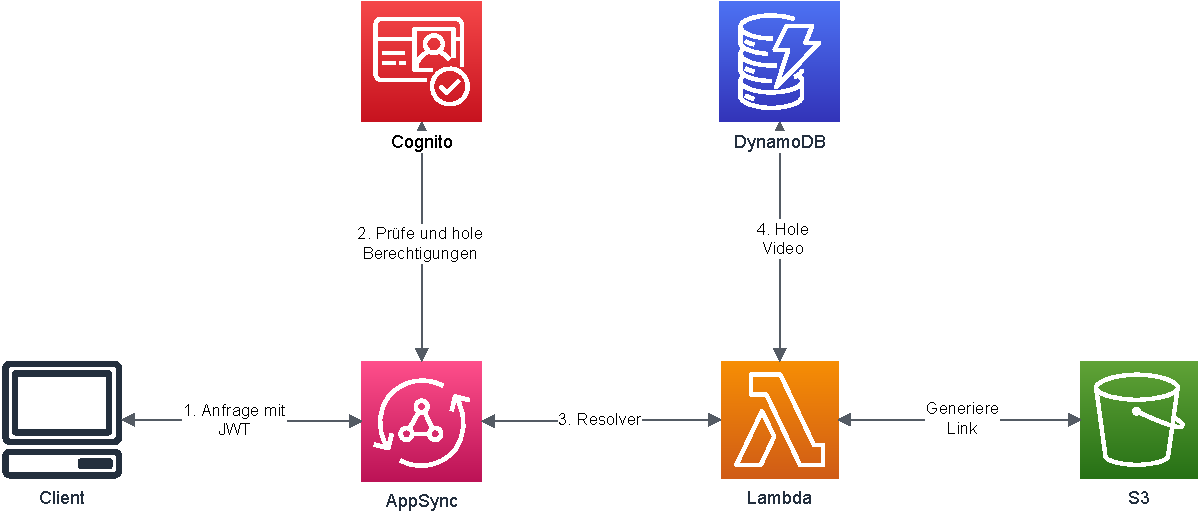
\includegraphics[width=1\columnwidth]{5_aws-amplify/laufzeitsicht_3.pdf}
  \caption{AWS Amplify - Laufzeitsicht - Erstellen von Links}
  \label{Amplify:laufzeitsicht2}
\end{figure}

\subsubsection{Erstellen eines Videos}

\autoref{Amplify:laufzeitsicht3} stellt den Prozess dar, wie ein Video erstellt wird.
\begin{enumerate}
  \item{Zunächst lädt der Nutzer das Video in den S3-Bucket hoch. Die Policy des S3-Buckets verwaltet den korrekten Zugriff auf die Ressource. Die hochgeladene Datei landet in einem privaten Ordner, der außerhalb des Backends ausschließlich für den Besitzer des Objekts aufrufbar ist. Das ist der Nutzer, der das Video hochgeladen hat.}
  \item{Erst dann erstellt der Nutzer eine Anfrage mittels GraphQL und dem JSON Webtoken.}
  \item{AppSync autorisiert den Nutzer und holt die Gruppenzugehörigkeit des Nutzers.}
  \item{Der Resolver führt die verknüpfte Lambda-Funktion aus.}
  \item{Die Funktion kopiert die hochgeladene Datei in einen weiteren Ordner, so dass der Besitzer diese nicht mehr verändern kann. Die hochgeladene Datei im Ursprungsordner wird daraufhin gelöscht.}
  \item{Die Funktion erstellt das Video in der DynamoDB-Tabelle.}
  \item{Die Funktion führt den MediaConvert-Job aus, um das Video mit dem Wasserzeichen zu versehen.}
  \item{Ist die Konvertierung abgeschlossen, benachrichtigt die EventBridge eine weitere Lambda-Funktion, welche das Video dann freischaltet.}
\end{enumerate}

\begin{figure}
  \centering
  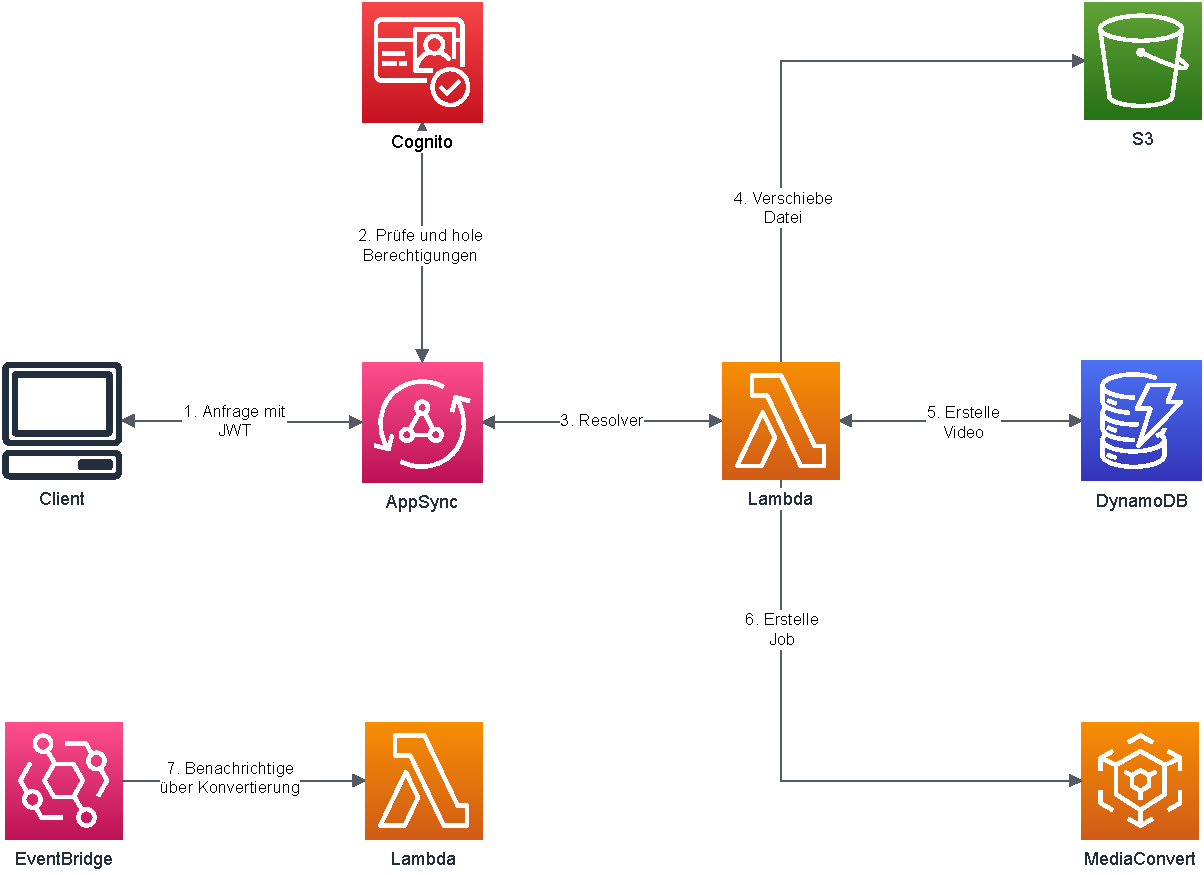
\includegraphics[width=1\columnwidth]{5_aws-amplify/laufzeitsicht_2.pdf}
  \caption{AWS Amplify - Laufzeitsicht - Erstellen eines Videos}
  \label{Amplify:laufzeitsicht3}
\end{figure}

\subsection{Verteilungssicht}

Die Verteilungssicht beschreibt, wie die Bausteine in \ac{AWS} über Stacks verteilt werden. Amplify bündelt die Verteilung des Backends und des Frontends über eine Pipeline. Diesen Sachverhalt stellt \autoref{Amplify:verteilungssicht} dar.

\begin{figure}
  \centering
  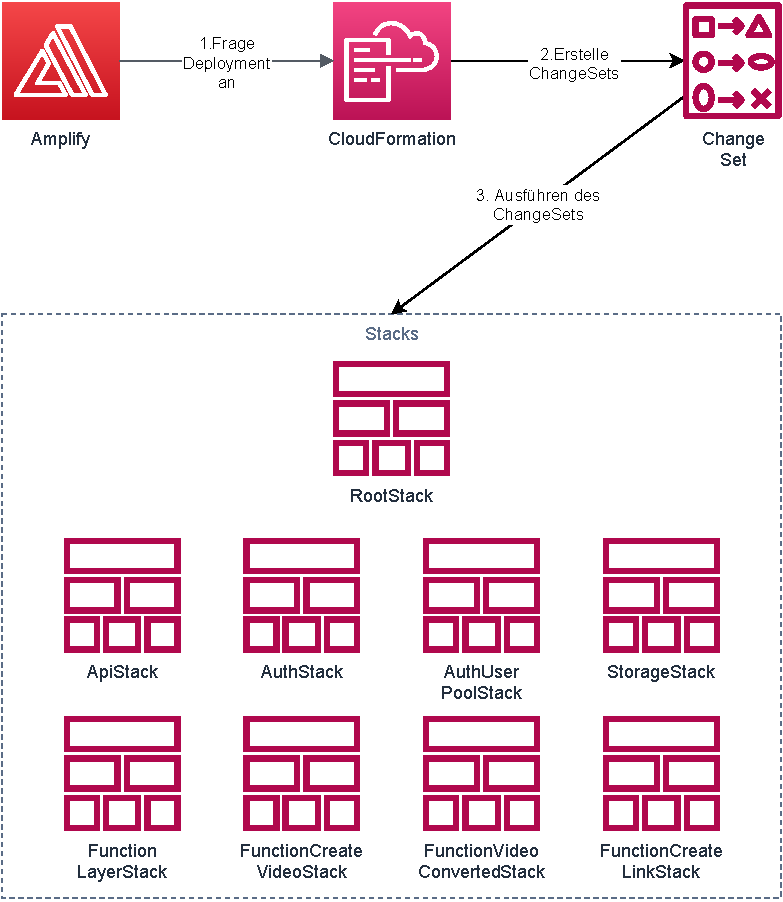
\includegraphics[width=0.75\columnwidth]{5_aws-amplify/verteilungssicht.pdf}
  \caption{AWS Amplify - Verteilungssicht}
  \label{Amplify:verteilungssicht}
\end{figure}

Amplify verteilt das Backend über die CloudFormation mittels Stacks. Außerdem werden nur Stacks und keine NestedStacks genutzt, was die Fehleranalyse vereinfacht. Um eine neue Änderung in das System einzuspielen, erzeugt die CloudFormation ein ChangeSet, welches die Differenz aus dem aktuellen Stand in der Cloud und dem gewünschten Zielzustand ist. Wenn beim Aktualisieren der Stacks ein Fehler auftritt, erfolgt ein Rollback.

Das Frontend wird separat, also nicht über Stacks, verteilt. Dazu nutzt Amplify einen gebündelten Dienst, der über die CloudFront läuft. Letzterer kann allerdings als Black-Box betrachtet werden, da der Entwickler diesen nur durch die Konfiguration beeinflussen kann.

\subsection{Querschnittliche Konzepte und Muster}

Logging
- CloudWatch

Backup
- AWS Backup

- Einbindung über \ac{AWS} Amplify:
  - AWS Elemental MediaConvert als extra Plugin
  - Anpassung an CF-Templates
- Permissions (IAM)

\subsection{Entwurfsentscheidungen}

\subsection{Risiken und technische Schulden}

- Auth: Anpassung, dass statt Identity ID die Pool User Id genutzt wird geht über https://github.com/aws-amplify/amplify-js/issues/54. Leider lässt sich das nicht persistieren, so dass man das bei jedem branch/Projekt neu eintragen muss. Wenn man es im CF-Template ändert, wird die Änderung beim Push rückgängig gemacht. Das ist nicht sehr flexibel. Ggf. Lösung finden und schauen, ob es doch geht.

- CDK als Alternative zu AWS Amplify, da es wesentlich flexibler

\section{Implementierung}

\chapter{AWS Amplify}

Das folgende Kapitel beschreibt die Architektur und die Implementierung mit Amplify.

\section{Architektur}

todo

\subsection{Lösungsstrategie}

Die Architektur folgt dem Aufbau einer Drei"=Schichten"=Architektur:
\begin{itemize}
  \item Präsentationsschicht
    \begin{itemize}
      \item React.js
      \item amplify-js
    \end{itemize}
  \item Logikschicht
    \begin{itemize}
      \item AppSync
      \item Lambda
      \item Cognito
      \item Elemental MediaConvert
      \item EventBridge
      \item IAM
    \end{itemize}
  \item Datenhaltungsschicht
    \begin{itemize}
      \item DynamoDB
      \item S3
      \item Cognito
      \item IAM
      \item AWS Backup
    \end{itemize}
\end{itemize}

Die Dienste Cognito und IAM befindet sich zugleich in zwei Schichten, da dort neben der Logik für Authentifizierung und Autorisierung auch die Benutzer persistiert werden.

Durch die ausschließliche Verwendung interner Dienste von \ac{AWS}, keiner Eigenentwicklungen für die Benutzerverwaltung und den vorgegebenen Technologien sind die Rahmenbedingungen für dieses Projekt nicht missachtet, so dass die beiden Technologien weiterhin vergleichbar sind.

\autoref{Kap2:NFAs} zeigt Lösungsansätze, um die nichtfunktionalen Anforderungen, auch Qualitätsziele genannt, zu erreichen.

\begin{table}[h]
  \caption{Lösungsansatz für nichtfunktionale Anforderungen}
  \label{Kap2:NFAs}
  \renewcommand{\arraystretch}{1.2}
  \centering
  \sffamily
  \begin{footnotesize}
    \begin{tabularx}{0.9\textwidth}{l l X}
      \toprule
      \textbf{Anforderung} & \textbf{Dienst} & \textbf{Ansatz}\\
      \midrule
        \emph{Verfügbarkeit} & Amplify & Amplify bietet für Frontend und Backend ein Zero-Downtime Deployment. \\
        \emph{Skalierbarkeit} & - & Durch die Serverless-Architektur skalieren Dienste automatisch innerhalb der \ac{AWS}-Cloud.\\
        \emph{Analysierbarkeit} & CloudWatch & Durch den Einsatz von CloudWatch können Anfragen für jeden Dienst nachvollzogen werden.\\
        \emph{Interoperabilität} & AppSync & Durch den Einsatz von AppSync ist mit GraphQL eine einheitliche Schnittstelle sichergestellt.\\
        \emph{Backups} & AWS Backup & Durch den Einsatz von AWS Backup werden automatisiert Backups aufgesetzt.\\
        \emph{Wiederherstellbarkeit} & AWS Backup &  Das von AWS Backup erstellte Backup für die Datenbank DynamoDB kann manuell eingespielt werden.\\
      \bottomrule
    \end{tabularx}
  \end{footnotesize}
  \rmfamily
\end{table}

\subsection{Bausteinsicht}

Die Architektur ist unterteilt in Frontend (Präsentationsschicht) und Backend (Logik- und Datenhaltungsschicht). Das Frontend wird nicht näher beschrieben, da Amplify dieses vollständig verwaltet. Das Backend besteht aus Stacks, welche zugleich den Code als auch die Infrastruktur repräsentieren. Diese werden im folgenden Abschnitt dargestellt:
\begin{itemize}
  \item{Der \textit{RootStack} enthält alle darunterliegenden Stacks sowie Ressourcen zum Deployment von Amplify.}

  \item{Der \textit{ApiStack} besteht aus den Diensten AppSync und DynamoDB. AppSync besteht aus einer GraphQLApi, die ein GraphQLSchema enthält. Außerdem nutzt AppSync Resolver, um ein Mapping über VTL zur DynamoDB-Tabelle zu ermöglichen. Um eine Verbindung zu einer Lambda-Funktion zu ermöglichen, existiert auch mindestens eine DataSource.}

  \item{Der \textit{AuthStack} regelt die Authentifizierung und Autorisierung von Benutzern über den Dienst Cognito. Dieser besteht aus einem UserPool und einem IdentityPool und den entsprechenden IAM-Rollen und Policies. Des weiteren besteht der Stack aus einem UserPoolClient, über welchen Anfragen auf Cognito erfolgen können. Amplify definiert auch weitere Lambda-Funktionen, um zusätzliche Logik für die Authentifizierung zu ermöglichen.}

  \item{Der \textit{AuthUserPoolGroupStack} dient zur Verwaltung der zusätzlichen UserPoolGroup für Administratoren.}

  \item{Der \textit{StorageStack} dient zur Speicherung der Videos. Dieser enthält einen S3-Bucket sowie eine dazugehören Policy, welchen es Benutzern ermöglicht, Dateien in eigene Ordner hochzuladen sowie andere Ordner lesen zu dürfen. Die Policy unterscheidet zwischen öffentlichen, geschützten und privaten Geltungsbereichen.}

  \item{Der \textit{FunctionLayerStack} bündelt die Node.js-Module als Lambda-Layer, den die weiteren Lambda-Funktionen nutzen.}

  \item{Der \textit{FunctionCreateVideoStack} übernimmt die Erstellung eines Videos in Form einer Lambda-Funktion. Außerdem erstellt der Stack in MediaConvert ein JobTemplate und eine Queue. Des Weiteren definiert der Stack die nötige Policy und Rolle, um der Lambda-Funktion die Zugriffe auf andere Dienste zu ermöglichen.}

  \item{Der \textit{FunctionVideoConvertedStack} besteht aus einer EventBridge-Regel, die bei einer Konvertierung eines Videos aufgerufen wird. Außerdem wird eine Lambda-Funktion mit der nötigen Policy und Rolle erstellt.}

  \item{Der \textit{FunctionCreateLinkStack} besteht aus einer Lambda-Funktion und der nötigen Rolle und Policy, um einen signierten zeitlich begrenzt gültigen Video-Link zu erstellen.}
\end{itemize}

Die Stacks \textit{RootStack}, \textit{ApiStack}, \textit{AuthStack}, \textit{AuthUserPoolGroupStack} und \textit{StorageStack} erstellt Amplify selbst. Die restlichen Stacks sind selbst erstellte bzw. angepasste Plugins, da die Dienste nicht vollständig in Amplify vorhanden sind.

\subsection{Laufzeitsicht}

Die Laufzeitsicht beschreibt die wichtigsten Prozesse und wie die Bausteine miteinander interagieren.

\subsubsection{Lesen, Aktualisieren und Löschen eines Videos}

\begin{figure}
  \centering
  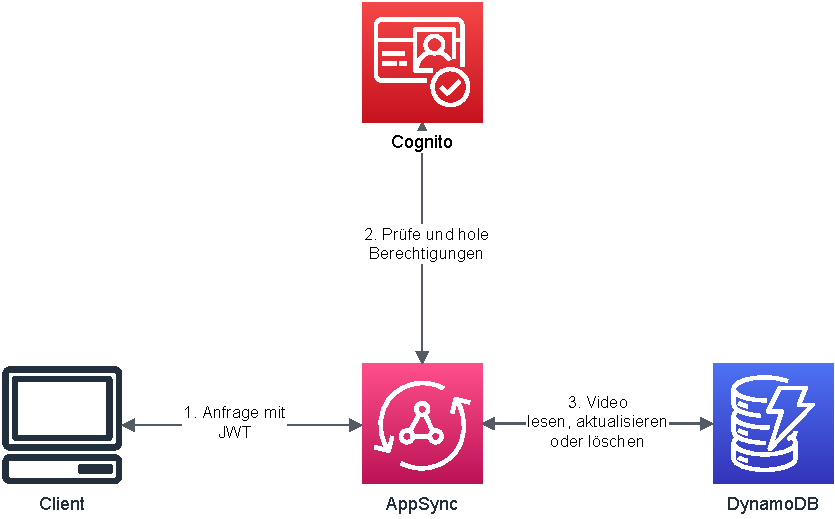
\includegraphics[width=0.75\columnwidth]{5_aws-amplify/laufzeitsicht_1.pdf}
  \caption{AWS Amplify - Laufzeitsicht - Lesen, Aktualisieren und Löschen eines Videos}
  \label{Amplify:laufzeitsicht1}
\end{figure}

\autoref{Amplify:laufzeitsicht1} stellt den Prozess dar, wie Videos von Nutzern gelesen, aktualisiert oder gelöscht werden. Dieser wird im folgenden Abschnitt näher erläutert:
\begin{enumerate}
  \item{Der Nutzer stellt eine Anfrage mittels GraphQL und dem JSON Webtoken.}
  \item{AppSync autorisiert den Nutzer und holt die Gruppenzugehörigkeit des Nutzers.}
  \item{Der Resolver leitet die Anfrage unter Berücksichtigung der Gruppenzugehörigkeit des Nutzers an DynamoDB weiter. Die nötigen Datenbankoperationen werden über DynamoDB ausgeführt.}
\end{enumerate}

Zusätzlich dazu müssen signierte temporäre Links erstellt werden, um die Sicherheit zu gewährleisten. Dieser Ablauf, der in \autoref{Amplify:laufzeitsicht2} dargestellt wird, enthält noch eine zusätzlich Abfrage auf S3, um den Link zu erstellen.

\begin{figure}
  \centering
  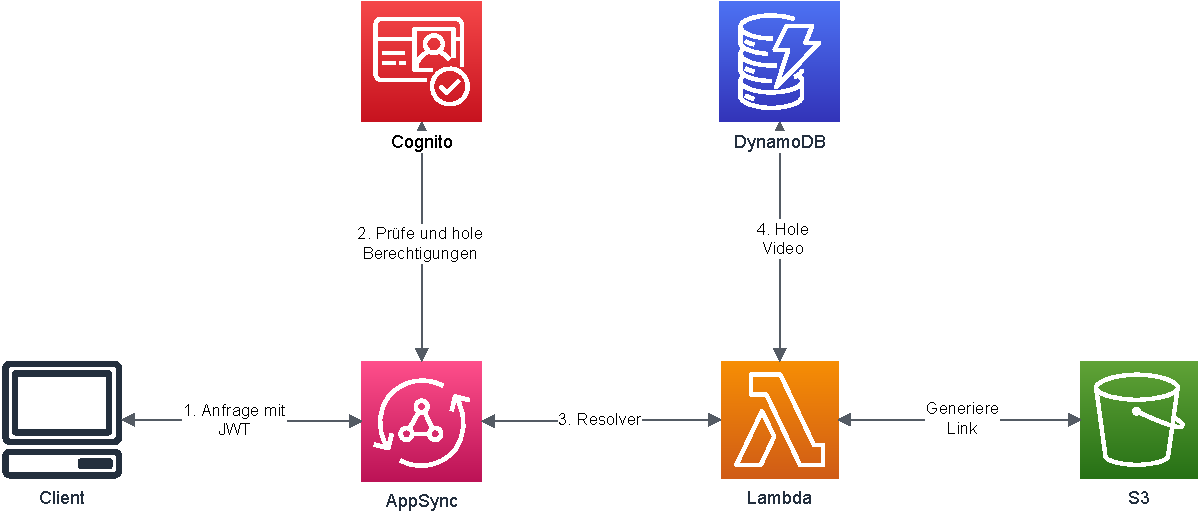
\includegraphics[width=1\columnwidth]{5_aws-amplify/laufzeitsicht_3.pdf}
  \caption{AWS Amplify - Laufzeitsicht - Erstellen von Links}
  \label{Amplify:laufzeitsicht2}
\end{figure}

\subsubsection{Erstellen eines Videos}

\autoref{Amplify:laufzeitsicht3} stellt den Prozess dar, wie ein Video erstellt wird.
\begin{enumerate}
  \item{Zunächst lädt der Nutzer das Video in den S3-Bucket hoch. Die Policy des S3-Buckets verwaltet den korrekten Zugriff auf die Ressource. Die hochgeladene Datei landet in einem privaten Ordner, der außerhalb des Backends ausschließlich für den Besitzer des Objekts aufrufbar ist. Das ist der Nutzer, der das Video hochgeladen hat.}
  \item{Erst dann erstellt der Nutzer eine Anfrage mittels GraphQL und dem JSON Webtoken.}
  \item{AppSync autorisiert den Nutzer und holt die Gruppenzugehörigkeit des Nutzers.}
  \item{Der Resolver führt die verknüpfte Lambda-Funktion aus.}
  \item{Die Funktion kopiert die hochgeladene Datei in einen weiteren Ordner, so dass der Besitzer diese nicht mehr verändern kann. Die hochgeladene Datei im Ursprungsordner wird daraufhin gelöscht.}
  \item{Die Funktion erstellt das Video in der DynamoDB-Tabelle.}
  \item{Die Funktion führt den MediaConvert-Job aus, um das Video mit dem Wasserzeichen zu versehen.}
  \item{Ist die Konvertierung abgeschlossen, benachrichtigt die EventBridge eine weitere Lambda-Funktion, welche das Video dann freischaltet.}
\end{enumerate}

\begin{figure}
  \centering
  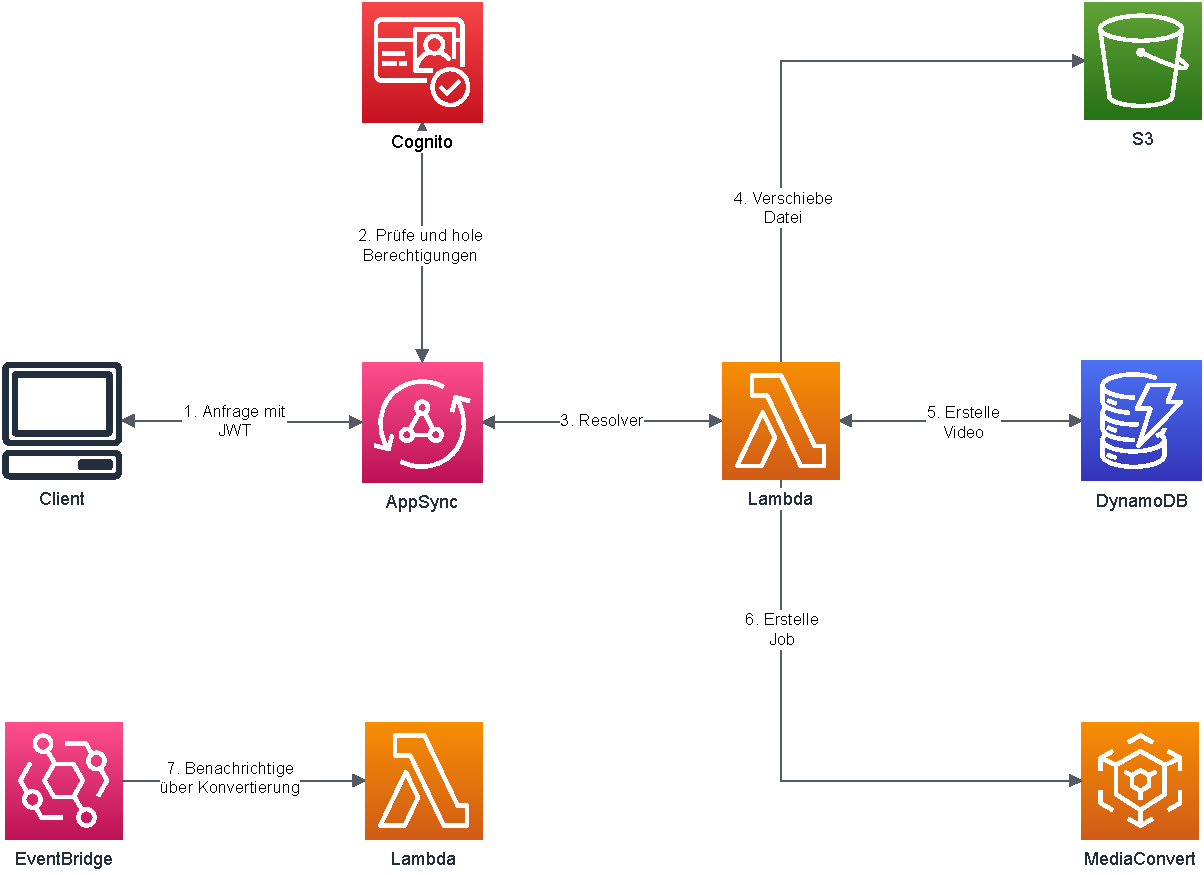
\includegraphics[width=1\columnwidth]{5_aws-amplify/laufzeitsicht_2.pdf}
  \caption{AWS Amplify - Laufzeitsicht - Erstellen eines Videos}
  \label{Amplify:laufzeitsicht3}
\end{figure}

\subsection{Verteilungssicht}

Die Verteilungssicht beschreibt, wie die Bausteine in \ac{AWS} über Stacks verteilt werden. Amplify bündelt die Verteilung des Backends und des Frontends über eine Pipeline. Diesen Sachverhalt stellt \autoref{Amplify:verteilungssicht} dar.

\begin{figure}
  \centering
  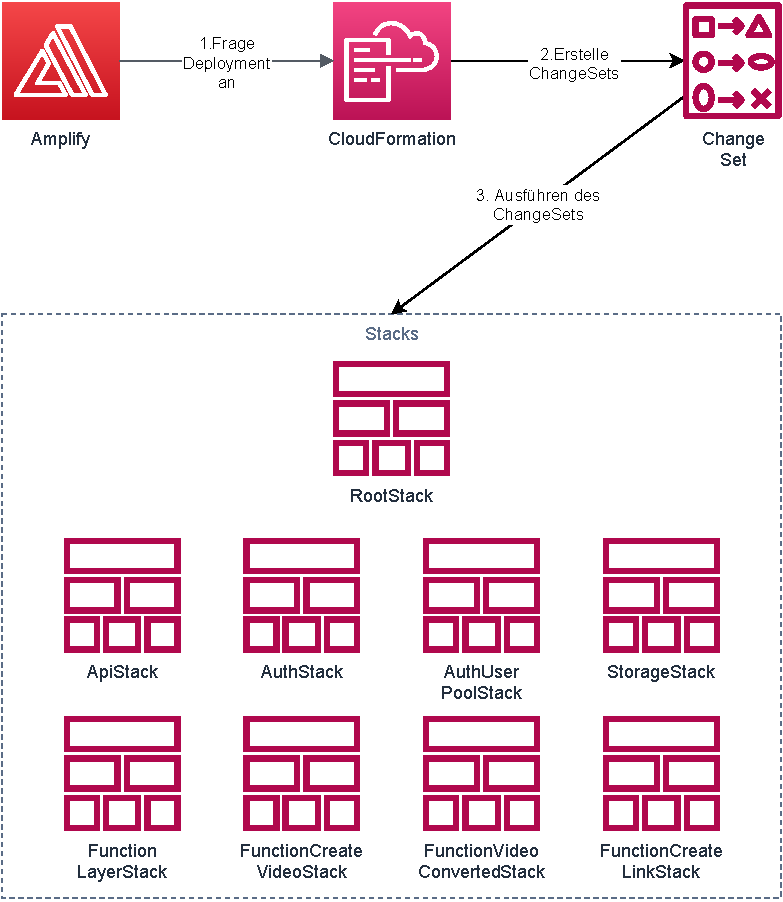
\includegraphics[width=0.75\columnwidth]{5_aws-amplify/verteilungssicht.pdf}
  \caption{AWS Amplify - Verteilungssicht}
  \label{Amplify:verteilungssicht}
\end{figure}

Amplify verteilt das Backend über die CloudFormation mittels Stacks. Außerdem werden nur Stacks und keine NestedStacks genutzt, was die Fehleranalyse vereinfacht. Um eine neue Änderung in das System einzuspielen, erzeugt die CloudFormation ein ChangeSet, welches die Differenz aus dem aktuellen Stand in der Cloud und dem gewünschten Zielzustand ist. Wenn beim Aktualisieren der Stacks ein Fehler auftritt, erfolgt ein Rollback.

Das Frontend wird separat, also nicht über Stacks, verteilt. Dazu nutzt Amplify einen gebündelten Dienst, der über die CloudFront läuft. Letzterer kann allerdings als Black-Box betrachtet werden, da der Entwickler diesen nur durch die Konfiguration beeinflussen kann.

\subsection{Querschnittliche Konzepte und Muster}

Logging
- CloudWatch

Backup
- AWS Backup

- Einbindung über \ac{AWS} Amplify:
  - AWS Elemental MediaConvert als extra Plugin
  - Anpassung an CF-Templates
- Permissions (IAM)

\subsection{Entwurfsentscheidungen}

\subsection{Risiken und technische Schulden}

- Auth: Anpassung, dass statt Identity ID die Pool User Id genutzt wird geht über https://github.com/aws-amplify/amplify-js/issues/54. Leider lässt sich das nicht persistieren, so dass man das bei jedem branch/Projekt neu eintragen muss. Wenn man es im CF-Template ändert, wird die Änderung beim Push rückgängig gemacht. Das ist nicht sehr flexibel. Ggf. Lösung finden und schauen, ob es doch geht.

- CDK als Alternative zu AWS Amplify, da es wesentlich flexibler

\section{Implementierung}

\chapter{AWS Amplify}

Das folgende Kapitel beschreibt die Architektur und die Implementierung mit Amplify.

\section{Architektur}

todo

\subsection{Lösungsstrategie}

Die Architektur folgt dem Aufbau einer Drei"=Schichten"=Architektur:
\begin{itemize}
  \item Präsentationsschicht
    \begin{itemize}
      \item React.js
      \item amplify-js
    \end{itemize}
  \item Logikschicht
    \begin{itemize}
      \item AppSync
      \item Lambda
      \item Cognito
      \item Elemental MediaConvert
      \item EventBridge
      \item IAM
    \end{itemize}
  \item Datenhaltungsschicht
    \begin{itemize}
      \item DynamoDB
      \item S3
      \item Cognito
      \item IAM
      \item AWS Backup
    \end{itemize}
\end{itemize}

Die Dienste Cognito und IAM befindet sich zugleich in zwei Schichten, da dort neben der Logik für Authentifizierung und Autorisierung auch die Benutzer persistiert werden.

Durch die ausschließliche Verwendung interner Dienste von \ac{AWS}, keiner Eigenentwicklungen für die Benutzerverwaltung und den vorgegebenen Technologien sind die Rahmenbedingungen für dieses Projekt nicht missachtet, so dass die beiden Technologien weiterhin vergleichbar sind.

\autoref{Kap2:NFAs} zeigt Lösungsansätze, um die nichtfunktionalen Anforderungen, auch Qualitätsziele genannt, zu erreichen.

\begin{table}[h]
  \caption{Lösungsansatz für nichtfunktionale Anforderungen}
  \label{Kap2:NFAs}
  \renewcommand{\arraystretch}{1.2}
  \centering
  \sffamily
  \begin{footnotesize}
    \begin{tabularx}{0.9\textwidth}{l l X}
      \toprule
      \textbf{Anforderung} & \textbf{Dienst} & \textbf{Ansatz}\\
      \midrule
        \emph{Verfügbarkeit} & Amplify & Amplify bietet für Frontend und Backend ein Zero-Downtime Deployment. \\
        \emph{Skalierbarkeit} & - & Durch die Serverless-Architektur skalieren Dienste automatisch innerhalb der \ac{AWS}-Cloud.\\
        \emph{Analysierbarkeit} & CloudWatch & Durch den Einsatz von CloudWatch können Anfragen für jeden Dienst nachvollzogen werden.\\
        \emph{Interoperabilität} & AppSync & Durch den Einsatz von AppSync ist mit GraphQL eine einheitliche Schnittstelle sichergestellt.\\
        \emph{Backups} & AWS Backup & Durch den Einsatz von AWS Backup werden automatisiert Backups aufgesetzt.\\
        \emph{Wiederherstellbarkeit} & AWS Backup &  Das von AWS Backup erstellte Backup für die Datenbank DynamoDB kann manuell eingespielt werden.\\
      \bottomrule
    \end{tabularx}
  \end{footnotesize}
  \rmfamily
\end{table}

\subsection{Bausteinsicht}

Die Architektur ist unterteilt in Frontend (Präsentationsschicht) und Backend (Logik- und Datenhaltungsschicht). Das Frontend wird nicht näher beschrieben, da Amplify dieses vollständig verwaltet. Das Backend besteht aus Stacks, welche zugleich den Code als auch die Infrastruktur repräsentieren. Diese werden im folgenden Abschnitt dargestellt:
\begin{itemize}
  \item{Der \textit{RootStack} enthält alle darunterliegenden Stacks sowie Ressourcen zum Deployment von Amplify.}

  \item{Der \textit{ApiStack} besteht aus den Diensten AppSync und DynamoDB. AppSync besteht aus einer GraphQLApi, die ein GraphQLSchema enthält. Außerdem nutzt AppSync Resolver, um ein Mapping über VTL zur DynamoDB-Tabelle zu ermöglichen. Um eine Verbindung zu einer Lambda-Funktion zu ermöglichen, existiert auch mindestens eine DataSource.}

  \item{Der \textit{AuthStack} regelt die Authentifizierung und Autorisierung von Benutzern über den Dienst Cognito. Dieser besteht aus einem UserPool und einem IdentityPool und den entsprechenden IAM-Rollen und Policies. Des weiteren besteht der Stack aus einem UserPoolClient, über welchen Anfragen auf Cognito erfolgen können. Amplify definiert auch weitere Lambda-Funktionen, um zusätzliche Logik für die Authentifizierung zu ermöglichen.}

  \item{Der \textit{AuthUserPoolGroupStack} dient zur Verwaltung der zusätzlichen UserPoolGroup für Administratoren.}

  \item{Der \textit{StorageStack} dient zur Speicherung der Videos. Dieser enthält einen S3-Bucket sowie eine dazugehören Policy, welchen es Benutzern ermöglicht, Dateien in eigene Ordner hochzuladen sowie andere Ordner lesen zu dürfen. Die Policy unterscheidet zwischen öffentlichen, geschützten und privaten Geltungsbereichen.}

  \item{Der \textit{FunctionLayerStack} bündelt die Node.js-Module als Lambda-Layer, den die weiteren Lambda-Funktionen nutzen.}

  \item{Der \textit{FunctionCreateVideoStack} übernimmt die Erstellung eines Videos in Form einer Lambda-Funktion. Außerdem erstellt der Stack in MediaConvert ein JobTemplate und eine Queue. Des Weiteren definiert der Stack die nötige Policy und Rolle, um der Lambda-Funktion die Zugriffe auf andere Dienste zu ermöglichen.}

  \item{Der \textit{FunctionVideoConvertedStack} besteht aus einer EventBridge-Regel, die bei einer Konvertierung eines Videos aufgerufen wird. Außerdem wird eine Lambda-Funktion mit der nötigen Policy und Rolle erstellt.}

  \item{Der \textit{FunctionCreateLinkStack} besteht aus einer Lambda-Funktion und der nötigen Rolle und Policy, um einen signierten zeitlich begrenzt gültigen Video-Link zu erstellen.}
\end{itemize}

Die Stacks \textit{RootStack}, \textit{ApiStack}, \textit{AuthStack}, \textit{AuthUserPoolGroupStack} und \textit{StorageStack} erstellt Amplify selbst. Die restlichen Stacks sind selbst erstellte bzw. angepasste Plugins, da die Dienste nicht vollständig in Amplify vorhanden sind.

\subsection{Laufzeitsicht}

Die Laufzeitsicht beschreibt die wichtigsten Prozesse und wie die Bausteine miteinander interagieren.

\subsubsection{Lesen, Aktualisieren und Löschen eines Videos}

\begin{figure}
  \centering
  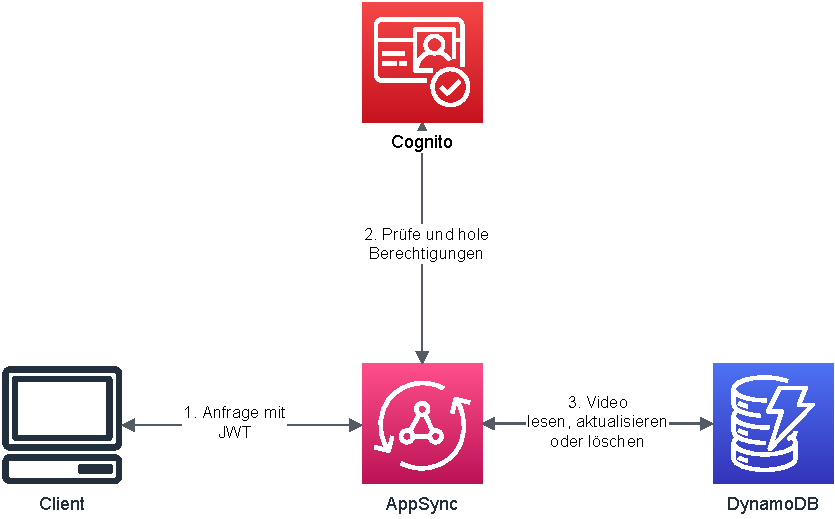
\includegraphics[width=0.75\columnwidth]{5_aws-amplify/laufzeitsicht_1.pdf}
  \caption{AWS Amplify - Laufzeitsicht - Lesen, Aktualisieren und Löschen eines Videos}
  \label{Amplify:laufzeitsicht1}
\end{figure}

\autoref{Amplify:laufzeitsicht1} stellt den Prozess dar, wie Videos von Nutzern gelesen, aktualisiert oder gelöscht werden. Dieser wird im folgenden Abschnitt näher erläutert:
\begin{enumerate}
  \item{Der Nutzer stellt eine Anfrage mittels GraphQL und dem JSON Webtoken.}
  \item{AppSync autorisiert den Nutzer und holt die Gruppenzugehörigkeit des Nutzers.}
  \item{Der Resolver leitet die Anfrage unter Berücksichtigung der Gruppenzugehörigkeit des Nutzers an DynamoDB weiter. Die nötigen Datenbankoperationen werden über DynamoDB ausgeführt.}
\end{enumerate}

Zusätzlich dazu müssen signierte temporäre Links erstellt werden, um die Sicherheit zu gewährleisten. Dieser Ablauf, der in \autoref{Amplify:laufzeitsicht2} dargestellt wird, enthält noch eine zusätzlich Abfrage auf S3, um den Link zu erstellen.

\begin{figure}
  \centering
  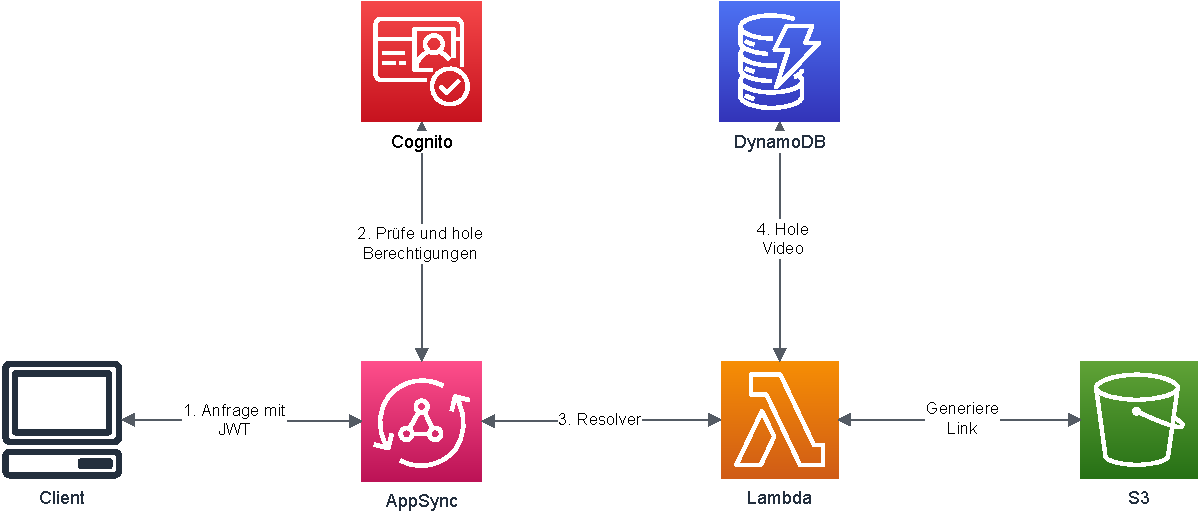
\includegraphics[width=1\columnwidth]{5_aws-amplify/laufzeitsicht_3.pdf}
  \caption{AWS Amplify - Laufzeitsicht - Erstellen von Links}
  \label{Amplify:laufzeitsicht2}
\end{figure}

\subsubsection{Erstellen eines Videos}

\autoref{Amplify:laufzeitsicht3} stellt den Prozess dar, wie ein Video erstellt wird.
\begin{enumerate}
  \item{Zunächst lädt der Nutzer das Video in den S3-Bucket hoch. Die Policy des S3-Buckets verwaltet den korrekten Zugriff auf die Ressource. Die hochgeladene Datei landet in einem privaten Ordner, der außerhalb des Backends ausschließlich für den Besitzer des Objekts aufrufbar ist. Das ist der Nutzer, der das Video hochgeladen hat.}
  \item{Erst dann erstellt der Nutzer eine Anfrage mittels GraphQL und dem JSON Webtoken.}
  \item{AppSync autorisiert den Nutzer und holt die Gruppenzugehörigkeit des Nutzers.}
  \item{Der Resolver führt die verknüpfte Lambda-Funktion aus.}
  \item{Die Funktion kopiert die hochgeladene Datei in einen weiteren Ordner, so dass der Besitzer diese nicht mehr verändern kann. Die hochgeladene Datei im Ursprungsordner wird daraufhin gelöscht.}
  \item{Die Funktion erstellt das Video in der DynamoDB-Tabelle.}
  \item{Die Funktion führt den MediaConvert-Job aus, um das Video mit dem Wasserzeichen zu versehen.}
  \item{Ist die Konvertierung abgeschlossen, benachrichtigt die EventBridge eine weitere Lambda-Funktion, welche das Video dann freischaltet.}
\end{enumerate}

\begin{figure}
  \centering
  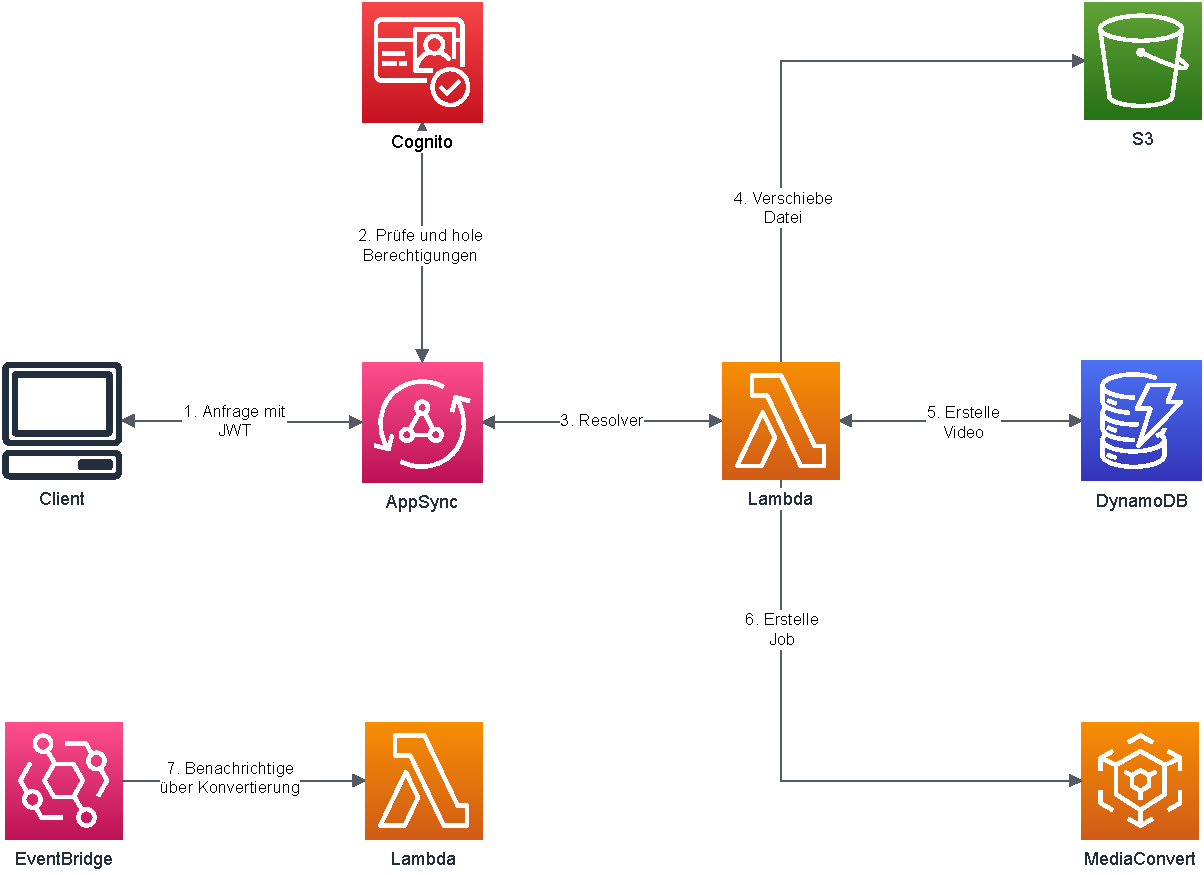
\includegraphics[width=1\columnwidth]{5_aws-amplify/laufzeitsicht_2.pdf}
  \caption{AWS Amplify - Laufzeitsicht - Erstellen eines Videos}
  \label{Amplify:laufzeitsicht3}
\end{figure}

\subsection{Verteilungssicht}

Die Verteilungssicht beschreibt, wie die Bausteine in \ac{AWS} über Stacks verteilt werden. Amplify bündelt die Verteilung des Backends und des Frontends über eine Pipeline. Diesen Sachverhalt stellt \autoref{Amplify:verteilungssicht} dar.

\begin{figure}
  \centering
  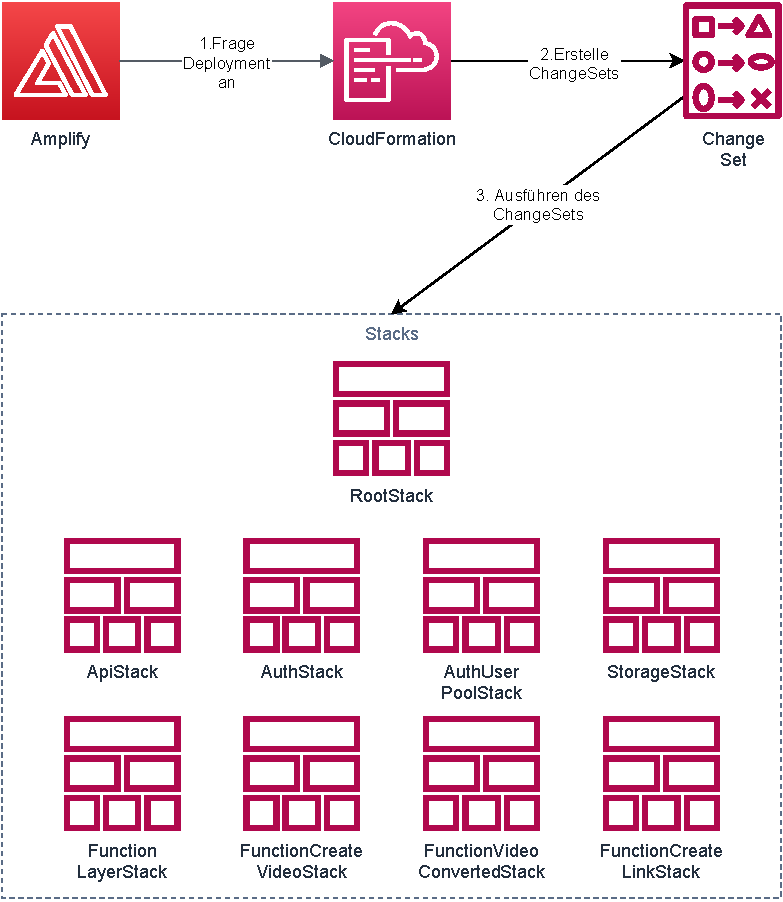
\includegraphics[width=0.75\columnwidth]{5_aws-amplify/verteilungssicht.pdf}
  \caption{AWS Amplify - Verteilungssicht}
  \label{Amplify:verteilungssicht}
\end{figure}

Amplify verteilt das Backend über die CloudFormation mittels Stacks. Außerdem werden nur Stacks und keine NestedStacks genutzt, was die Fehleranalyse vereinfacht. Um eine neue Änderung in das System einzuspielen, erzeugt die CloudFormation ein ChangeSet, welches die Differenz aus dem aktuellen Stand in der Cloud und dem gewünschten Zielzustand ist. Wenn beim Aktualisieren der Stacks ein Fehler auftritt, erfolgt ein Rollback.

Das Frontend wird separat, also nicht über Stacks, verteilt. Dazu nutzt Amplify einen gebündelten Dienst, der über die CloudFront läuft. Letzterer kann allerdings als Black-Box betrachtet werden, da der Entwickler diesen nur durch die Konfiguration beeinflussen kann.

\subsection{Querschnittliche Konzepte und Muster}

Logging
- CloudWatch

Backup
- AWS Backup

- Einbindung über \ac{AWS} Amplify:
  - AWS Elemental MediaConvert als extra Plugin
  - Anpassung an CF-Templates
- Permissions (IAM)

\subsection{Entwurfsentscheidungen}

\subsection{Risiken und technische Schulden}

- Auth: Anpassung, dass statt Identity ID die Pool User Id genutzt wird geht über https://github.com/aws-amplify/amplify-js/issues/54. Leider lässt sich das nicht persistieren, so dass man das bei jedem branch/Projekt neu eintragen muss. Wenn man es im CF-Template ändert, wird die Änderung beim Push rückgängig gemacht. Das ist nicht sehr flexibel. Ggf. Lösung finden und schauen, ob es doch geht.

- CDK als Alternative zu AWS Amplify, da es wesentlich flexibler

\section{Implementierung}

\chapter{AWS Amplify}

Das folgende Kapitel beschreibt die Architektur und die Implementierung mit Amplify.

\section{Architektur}

todo

\subsection{Lösungsstrategie}

Die Architektur folgt dem Aufbau einer Drei"=Schichten"=Architektur:
\begin{itemize}
  \item Präsentationsschicht
    \begin{itemize}
      \item React.js
      \item amplify-js
    \end{itemize}
  \item Logikschicht
    \begin{itemize}
      \item AppSync
      \item Lambda
      \item Cognito
      \item Elemental MediaConvert
      \item EventBridge
      \item IAM
    \end{itemize}
  \item Datenhaltungsschicht
    \begin{itemize}
      \item DynamoDB
      \item S3
      \item Cognito
      \item IAM
      \item AWS Backup
    \end{itemize}
\end{itemize}

Die Dienste Cognito und IAM befindet sich zugleich in zwei Schichten, da dort neben der Logik für Authentifizierung und Autorisierung auch die Benutzer persistiert werden.

Durch die ausschließliche Verwendung interner Dienste von \ac{AWS}, keiner Eigenentwicklungen für die Benutzerverwaltung und den vorgegebenen Technologien sind die Rahmenbedingungen für dieses Projekt nicht missachtet, so dass die beiden Technologien weiterhin vergleichbar sind.

\autoref{Kap2:NFAs} zeigt Lösungsansätze, um die nichtfunktionalen Anforderungen, auch Qualitätsziele genannt, zu erreichen.

\begin{table}[h]
  \caption{Lösungsansatz für nichtfunktionale Anforderungen}
  \label{Kap2:NFAs}
  \renewcommand{\arraystretch}{1.2}
  \centering
  \sffamily
  \begin{footnotesize}
    \begin{tabularx}{0.9\textwidth}{l l X}
      \toprule
      \textbf{Anforderung} & \textbf{Dienst} & \textbf{Ansatz}\\
      \midrule
        \emph{Verfügbarkeit} & Amplify & Amplify bietet für Frontend und Backend ein Zero-Downtime Deployment. \\
        \emph{Skalierbarkeit} & - & Durch die Serverless-Architektur skalieren Dienste automatisch innerhalb der \ac{AWS}-Cloud.\\
        \emph{Analysierbarkeit} & CloudWatch & Durch den Einsatz von CloudWatch können Anfragen für jeden Dienst nachvollzogen werden.\\
        \emph{Interoperabilität} & AppSync & Durch den Einsatz von AppSync ist mit GraphQL eine einheitliche Schnittstelle sichergestellt.\\
        \emph{Backups} & AWS Backup & Durch den Einsatz von AWS Backup werden automatisiert Backups aufgesetzt.\\
        \emph{Wiederherstellbarkeit} & AWS Backup &  Das von AWS Backup erstellte Backup für die Datenbank DynamoDB kann manuell eingespielt werden.\\
      \bottomrule
    \end{tabularx}
  \end{footnotesize}
  \rmfamily
\end{table}

\subsection{Bausteinsicht}

Die Architektur ist unterteilt in Frontend (Präsentationsschicht) und Backend (Logik- und Datenhaltungsschicht). Das Frontend wird nicht näher beschrieben, da Amplify dieses vollständig verwaltet. Das Backend besteht aus Stacks, welche zugleich den Code als auch die Infrastruktur repräsentieren. Diese werden im folgenden Abschnitt dargestellt:
\begin{itemize}
  \item{Der \textit{RootStack} enthält alle darunterliegenden Stacks sowie Ressourcen zum Deployment von Amplify.}

  \item{Der \textit{ApiStack} besteht aus den Diensten AppSync und DynamoDB. AppSync besteht aus einer GraphQLApi, die ein GraphQLSchema enthält. Außerdem nutzt AppSync Resolver, um ein Mapping über VTL zur DynamoDB-Tabelle zu ermöglichen. Um eine Verbindung zu einer Lambda-Funktion zu ermöglichen, existiert auch mindestens eine DataSource.}

  \item{Der \textit{AuthStack} regelt die Authentifizierung und Autorisierung von Benutzern über den Dienst Cognito. Dieser besteht aus einem UserPool und einem IdentityPool und den entsprechenden IAM-Rollen und Policies. Des weiteren besteht der Stack aus einem UserPoolClient, über welchen Anfragen auf Cognito erfolgen können. Amplify definiert auch weitere Lambda-Funktionen, um zusätzliche Logik für die Authentifizierung zu ermöglichen.}

  \item{Der \textit{AuthUserPoolGroupStack} dient zur Verwaltung der zusätzlichen UserPoolGroup für Administratoren.}

  \item{Der \textit{StorageStack} dient zur Speicherung der Videos. Dieser enthält einen S3-Bucket sowie eine dazugehören Policy, welchen es Benutzern ermöglicht, Dateien in eigene Ordner hochzuladen sowie andere Ordner lesen zu dürfen. Die Policy unterscheidet zwischen öffentlichen, geschützten und privaten Geltungsbereichen.}

  \item{Der \textit{FunctionLayerStack} bündelt die Node.js-Module als Lambda-Layer, den die weiteren Lambda-Funktionen nutzen.}

  \item{Der \textit{FunctionCreateVideoStack} übernimmt die Erstellung eines Videos in Form einer Lambda-Funktion. Außerdem erstellt der Stack in MediaConvert ein JobTemplate und eine Queue. Des Weiteren definiert der Stack die nötige Policy und Rolle, um der Lambda-Funktion die Zugriffe auf andere Dienste zu ermöglichen.}

  \item{Der \textit{FunctionVideoConvertedStack} besteht aus einer EventBridge-Regel, die bei einer Konvertierung eines Videos aufgerufen wird. Außerdem wird eine Lambda-Funktion mit der nötigen Policy und Rolle erstellt.}

  \item{Der \textit{FunctionCreateLinkStack} besteht aus einer Lambda-Funktion und der nötigen Rolle und Policy, um einen signierten zeitlich begrenzt gültigen Video-Link zu erstellen.}
\end{itemize}

Die Stacks \textit{RootStack}, \textit{ApiStack}, \textit{AuthStack}, \textit{AuthUserPoolGroupStack} und \textit{StorageStack} erstellt Amplify selbst. Die restlichen Stacks sind selbst erstellte bzw. angepasste Plugins, da die Dienste nicht vollständig in Amplify vorhanden sind.

\subsection{Laufzeitsicht}

Die Laufzeitsicht beschreibt die wichtigsten Prozesse und wie die Bausteine miteinander interagieren.

\subsubsection{Lesen, Aktualisieren und Löschen eines Videos}

\begin{figure}
  \centering
  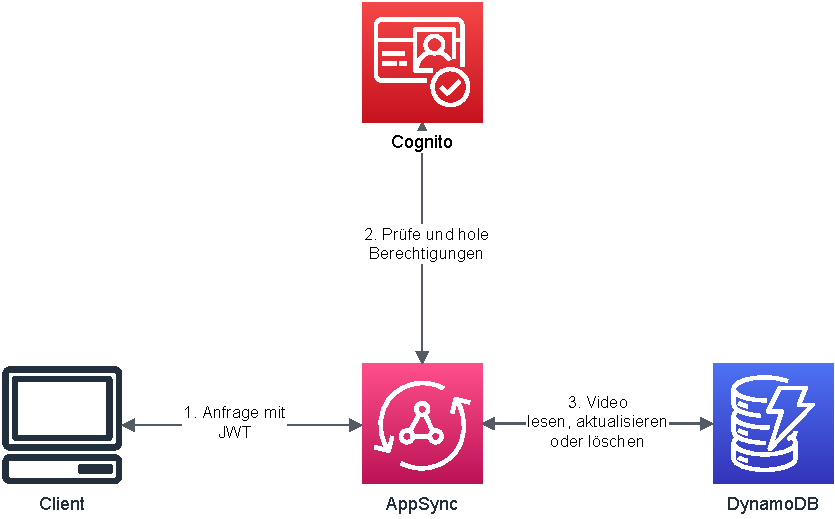
\includegraphics[width=0.75\columnwidth]{5_aws-amplify/laufzeitsicht_1.pdf}
  \caption{AWS Amplify - Laufzeitsicht - Lesen, Aktualisieren und Löschen eines Videos}
  \label{Amplify:laufzeitsicht1}
\end{figure}

\autoref{Amplify:laufzeitsicht1} stellt den Prozess dar, wie Videos von Nutzern gelesen, aktualisiert oder gelöscht werden. Dieser wird im folgenden Abschnitt näher erläutert:
\begin{enumerate}
  \item{Der Nutzer stellt eine Anfrage mittels GraphQL und dem JSON Webtoken.}
  \item{AppSync autorisiert den Nutzer und holt die Gruppenzugehörigkeit des Nutzers.}
  \item{Der Resolver leitet die Anfrage unter Berücksichtigung der Gruppenzugehörigkeit des Nutzers an DynamoDB weiter. Die nötigen Datenbankoperationen werden über DynamoDB ausgeführt.}
\end{enumerate}

Zusätzlich dazu müssen signierte temporäre Links erstellt werden, um die Sicherheit zu gewährleisten. Dieser Ablauf, der in \autoref{Amplify:laufzeitsicht2} dargestellt wird, enthält noch eine zusätzlich Abfrage auf S3, um den Link zu erstellen.

\begin{figure}
  \centering
  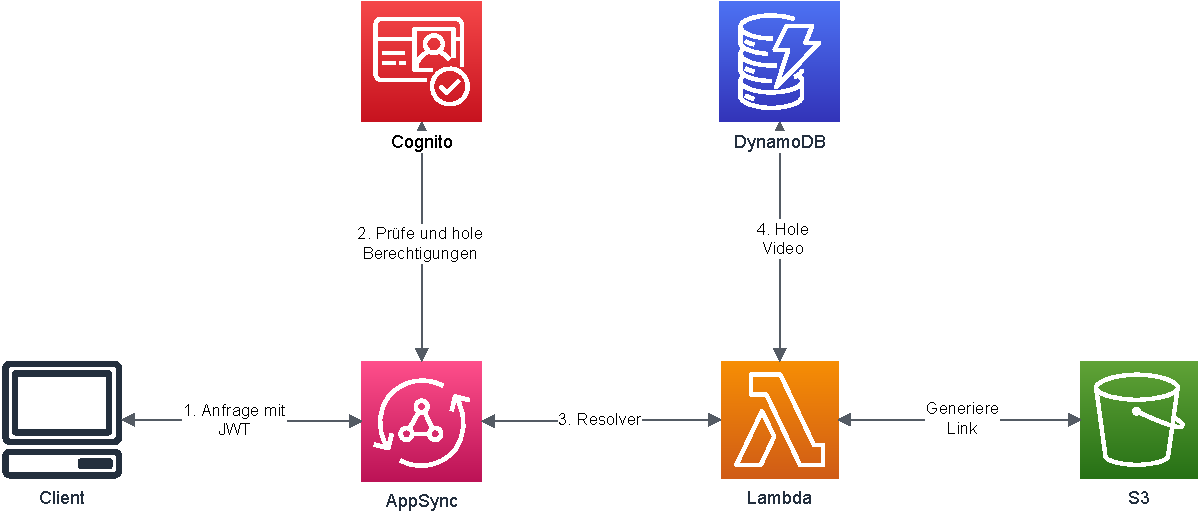
\includegraphics[width=1\columnwidth]{5_aws-amplify/laufzeitsicht_3.pdf}
  \caption{AWS Amplify - Laufzeitsicht - Erstellen von Links}
  \label{Amplify:laufzeitsicht2}
\end{figure}

\subsubsection{Erstellen eines Videos}

\autoref{Amplify:laufzeitsicht3} stellt den Prozess dar, wie ein Video erstellt wird.
\begin{enumerate}
  \item{Zunächst lädt der Nutzer das Video in den S3-Bucket hoch. Die Policy des S3-Buckets verwaltet den korrekten Zugriff auf die Ressource. Die hochgeladene Datei landet in einem privaten Ordner, der außerhalb des Backends ausschließlich für den Besitzer des Objekts aufrufbar ist. Das ist der Nutzer, der das Video hochgeladen hat.}
  \item{Erst dann erstellt der Nutzer eine Anfrage mittels GraphQL und dem JSON Webtoken.}
  \item{AppSync autorisiert den Nutzer und holt die Gruppenzugehörigkeit des Nutzers.}
  \item{Der Resolver führt die verknüpfte Lambda-Funktion aus.}
  \item{Die Funktion kopiert die hochgeladene Datei in einen weiteren Ordner, so dass der Besitzer diese nicht mehr verändern kann. Die hochgeladene Datei im Ursprungsordner wird daraufhin gelöscht.}
  \item{Die Funktion erstellt das Video in der DynamoDB-Tabelle.}
  \item{Die Funktion führt den MediaConvert-Job aus, um das Video mit dem Wasserzeichen zu versehen.}
  \item{Ist die Konvertierung abgeschlossen, benachrichtigt die EventBridge eine weitere Lambda-Funktion, welche das Video dann freischaltet.}
\end{enumerate}

\begin{figure}
  \centering
  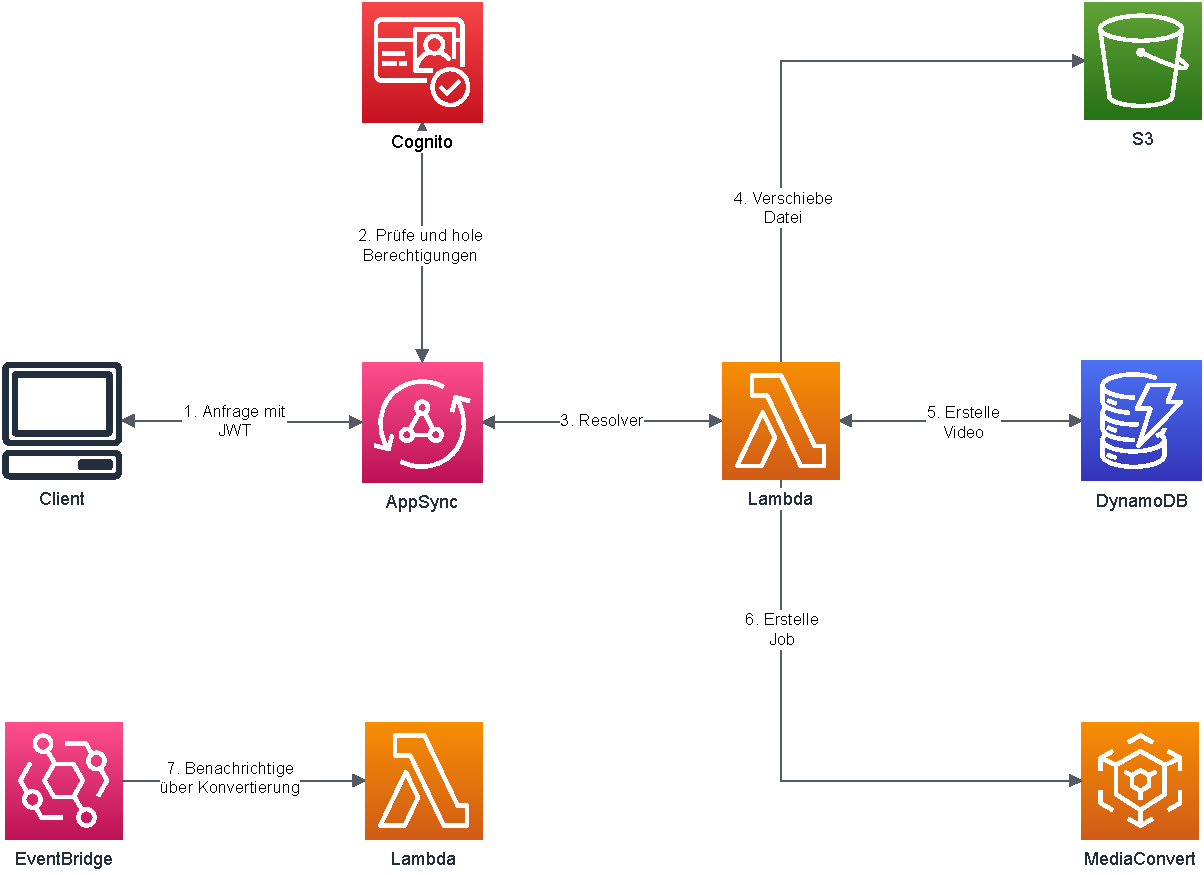
\includegraphics[width=1\columnwidth]{5_aws-amplify/laufzeitsicht_2.pdf}
  \caption{AWS Amplify - Laufzeitsicht - Erstellen eines Videos}
  \label{Amplify:laufzeitsicht3}
\end{figure}

\subsection{Verteilungssicht}

Die Verteilungssicht beschreibt, wie die Bausteine in \ac{AWS} über Stacks verteilt werden. Amplify bündelt die Verteilung des Backends und des Frontends über eine Pipeline. Diesen Sachverhalt stellt \autoref{Amplify:verteilungssicht} dar.

\begin{figure}
  \centering
  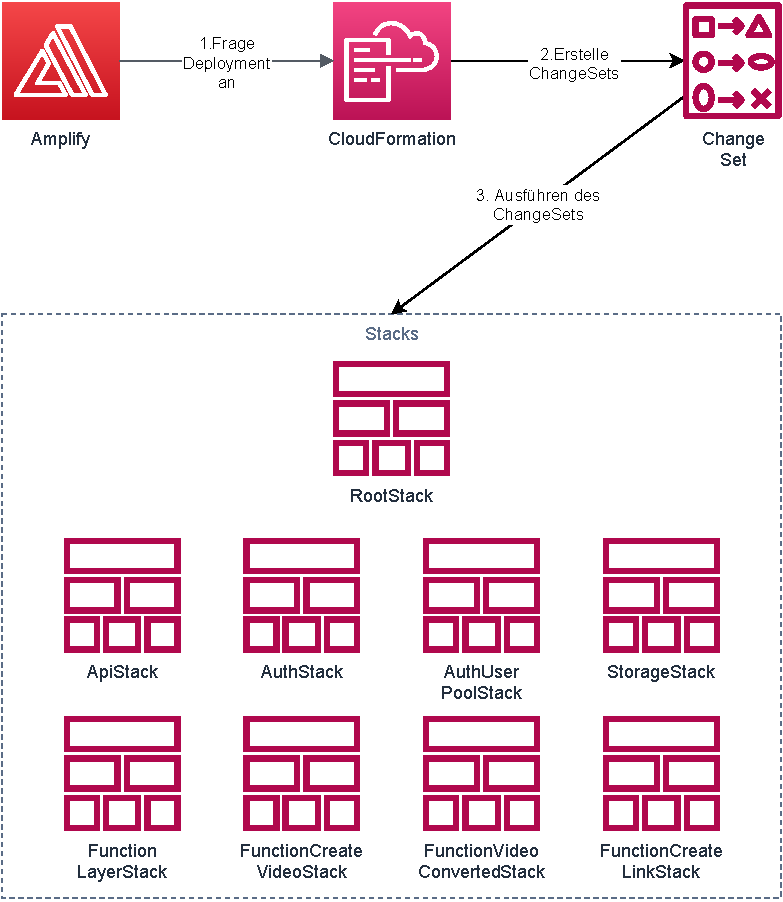
\includegraphics[width=0.75\columnwidth]{5_aws-amplify/verteilungssicht.pdf}
  \caption{AWS Amplify - Verteilungssicht}
  \label{Amplify:verteilungssicht}
\end{figure}

Amplify verteilt das Backend über die CloudFormation mittels Stacks. Außerdem werden nur Stacks und keine NestedStacks genutzt, was die Fehleranalyse vereinfacht. Um eine neue Änderung in das System einzuspielen, erzeugt die CloudFormation ein ChangeSet, welches die Differenz aus dem aktuellen Stand in der Cloud und dem gewünschten Zielzustand ist. Wenn beim Aktualisieren der Stacks ein Fehler auftritt, erfolgt ein Rollback.

Das Frontend wird separat, also nicht über Stacks, verteilt. Dazu nutzt Amplify einen gebündelten Dienst, der über die CloudFront läuft. Letzterer kann allerdings als Black-Box betrachtet werden, da der Entwickler diesen nur durch die Konfiguration beeinflussen kann.

\subsection{Querschnittliche Konzepte und Muster}

Logging
- CloudWatch

Backup
- AWS Backup

- Einbindung über \ac{AWS} Amplify:
  - AWS Elemental MediaConvert als extra Plugin
  - Anpassung an CF-Templates
- Permissions (IAM)

\subsection{Entwurfsentscheidungen}

\subsection{Risiken und technische Schulden}

- Auth: Anpassung, dass statt Identity ID die Pool User Id genutzt wird geht über https://github.com/aws-amplify/amplify-js/issues/54. Leider lässt sich das nicht persistieren, so dass man das bei jedem branch/Projekt neu eintragen muss. Wenn man es im CF-Template ändert, wird die Änderung beim Push rückgängig gemacht. Das ist nicht sehr flexibel. Ggf. Lösung finden und schauen, ob es doch geht.

- CDK als Alternative zu AWS Amplify, da es wesentlich flexibler

\section{Implementierung}

\chapter{AWS Amplify}

Das folgende Kapitel beschreibt die Architektur und die Implementierung mit Amplify.

\section{Architektur}

todo

\subsection{Lösungsstrategie}

Die Architektur folgt dem Aufbau einer Drei"=Schichten"=Architektur:
\begin{itemize}
  \item Präsentationsschicht
    \begin{itemize}
      \item React.js
      \item amplify-js
    \end{itemize}
  \item Logikschicht
    \begin{itemize}
      \item AppSync
      \item Lambda
      \item Cognito
      \item Elemental MediaConvert
      \item EventBridge
      \item IAM
    \end{itemize}
  \item Datenhaltungsschicht
    \begin{itemize}
      \item DynamoDB
      \item S3
      \item Cognito
      \item IAM
      \item AWS Backup
    \end{itemize}
\end{itemize}

Die Dienste Cognito und IAM befindet sich zugleich in zwei Schichten, da dort neben der Logik für Authentifizierung und Autorisierung auch die Benutzer persistiert werden.

Durch die ausschließliche Verwendung interner Dienste von \ac{AWS}, keiner Eigenentwicklungen für die Benutzerverwaltung und den vorgegebenen Technologien sind die Rahmenbedingungen für dieses Projekt nicht missachtet, so dass die beiden Technologien weiterhin vergleichbar sind.

\autoref{Kap2:NFAs} zeigt Lösungsansätze, um die nichtfunktionalen Anforderungen, auch Qualitätsziele genannt, zu erreichen.

\begin{table}[h]
  \caption{Lösungsansatz für nichtfunktionale Anforderungen}
  \label{Kap2:NFAs}
  \renewcommand{\arraystretch}{1.2}
  \centering
  \sffamily
  \begin{footnotesize}
    \begin{tabularx}{0.9\textwidth}{l l X}
      \toprule
      \textbf{Anforderung} & \textbf{Dienst} & \textbf{Ansatz}\\
      \midrule
        \emph{Verfügbarkeit} & Amplify & Amplify bietet für Frontend und Backend ein Zero-Downtime Deployment. \\
        \emph{Skalierbarkeit} & - & Durch die Serverless-Architektur skalieren Dienste automatisch innerhalb der \ac{AWS}-Cloud.\\
        \emph{Analysierbarkeit} & CloudWatch & Durch den Einsatz von CloudWatch können Anfragen für jeden Dienst nachvollzogen werden.\\
        \emph{Interoperabilität} & AppSync & Durch den Einsatz von AppSync ist mit GraphQL eine einheitliche Schnittstelle sichergestellt.\\
        \emph{Backups} & AWS Backup & Durch den Einsatz von AWS Backup werden automatisiert Backups aufgesetzt.\\
        \emph{Wiederherstellbarkeit} & AWS Backup &  Das von AWS Backup erstellte Backup für die Datenbank DynamoDB kann manuell eingespielt werden.\\
      \bottomrule
    \end{tabularx}
  \end{footnotesize}
  \rmfamily
\end{table}

\subsection{Bausteinsicht}

Die Architektur ist unterteilt in Frontend (Präsentationsschicht) und Backend (Logik- und Datenhaltungsschicht). Das Frontend wird nicht näher beschrieben, da Amplify dieses vollständig verwaltet. Das Backend besteht aus Stacks, welche zugleich den Code als auch die Infrastruktur repräsentieren. Diese werden im folgenden Abschnitt dargestellt:
\begin{itemize}
  \item{Der \textit{RootStack} enthält alle darunterliegenden Stacks sowie Ressourcen zum Deployment von Amplify.}

  \item{Der \textit{ApiStack} besteht aus den Diensten AppSync und DynamoDB. AppSync besteht aus einer GraphQLApi, die ein GraphQLSchema enthält. Außerdem nutzt AppSync Resolver, um ein Mapping über VTL zur DynamoDB-Tabelle zu ermöglichen. Um eine Verbindung zu einer Lambda-Funktion zu ermöglichen, existiert auch mindestens eine DataSource.}

  \item{Der \textit{AuthStack} regelt die Authentifizierung und Autorisierung von Benutzern über den Dienst Cognito. Dieser besteht aus einem UserPool und einem IdentityPool und den entsprechenden IAM-Rollen und Policies. Des weiteren besteht der Stack aus einem UserPoolClient, über welchen Anfragen auf Cognito erfolgen können. Amplify definiert auch weitere Lambda-Funktionen, um zusätzliche Logik für die Authentifizierung zu ermöglichen.}

  \item{Der \textit{AuthUserPoolGroupStack} dient zur Verwaltung der zusätzlichen UserPoolGroup für Administratoren.}

  \item{Der \textit{StorageStack} dient zur Speicherung der Videos. Dieser enthält einen S3-Bucket sowie eine dazugehören Policy, welchen es Benutzern ermöglicht, Dateien in eigene Ordner hochzuladen sowie andere Ordner lesen zu dürfen. Die Policy unterscheidet zwischen öffentlichen, geschützten und privaten Geltungsbereichen.}

  \item{Der \textit{FunctionLayerStack} bündelt die Node.js-Module als Lambda-Layer, den die weiteren Lambda-Funktionen nutzen.}

  \item{Der \textit{FunctionCreateVideoStack} übernimmt die Erstellung eines Videos in Form einer Lambda-Funktion. Außerdem erstellt der Stack in MediaConvert ein JobTemplate und eine Queue. Des Weiteren definiert der Stack die nötige Policy und Rolle, um der Lambda-Funktion die Zugriffe auf andere Dienste zu ermöglichen.}

  \item{Der \textit{FunctionVideoConvertedStack} besteht aus einer EventBridge-Regel, die bei einer Konvertierung eines Videos aufgerufen wird. Außerdem wird eine Lambda-Funktion mit der nötigen Policy und Rolle erstellt.}

  \item{Der \textit{FunctionCreateLinkStack} besteht aus einer Lambda-Funktion und der nötigen Rolle und Policy, um einen signierten zeitlich begrenzt gültigen Video-Link zu erstellen.}
\end{itemize}

Die Stacks \textit{RootStack}, \textit{ApiStack}, \textit{AuthStack}, \textit{AuthUserPoolGroupStack} und \textit{StorageStack} erstellt Amplify selbst. Die restlichen Stacks sind selbst erstellte bzw. angepasste Plugins, da die Dienste nicht vollständig in Amplify vorhanden sind.

\subsection{Laufzeitsicht}

Die Laufzeitsicht beschreibt die wichtigsten Prozesse und wie die Bausteine miteinander interagieren.

\subsubsection{Lesen, Aktualisieren und Löschen eines Videos}

\begin{figure}
  \centering
  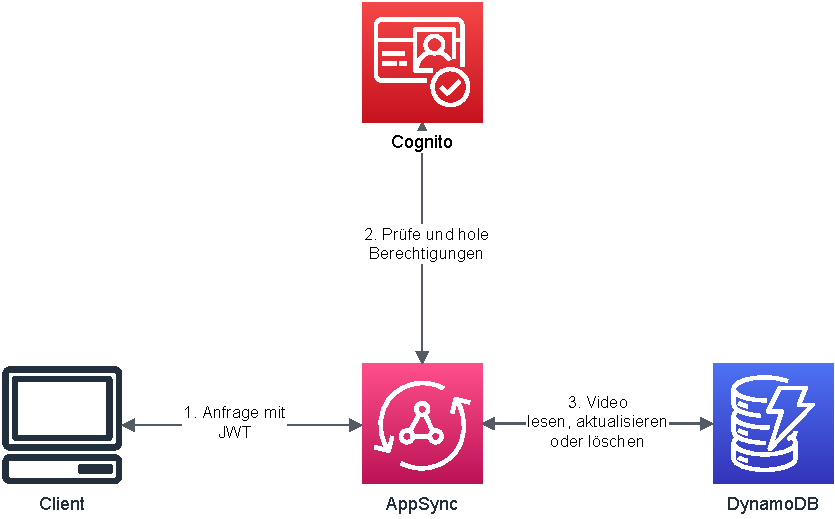
\includegraphics[width=0.75\columnwidth]{5_aws-amplify/laufzeitsicht_1.pdf}
  \caption{AWS Amplify - Laufzeitsicht - Lesen, Aktualisieren und Löschen eines Videos}
  \label{Amplify:laufzeitsicht1}
\end{figure}

\autoref{Amplify:laufzeitsicht1} stellt den Prozess dar, wie Videos von Nutzern gelesen, aktualisiert oder gelöscht werden. Dieser wird im folgenden Abschnitt näher erläutert:
\begin{enumerate}
  \item{Der Nutzer stellt eine Anfrage mittels GraphQL und dem JSON Webtoken.}
  \item{AppSync autorisiert den Nutzer und holt die Gruppenzugehörigkeit des Nutzers.}
  \item{Der Resolver leitet die Anfrage unter Berücksichtigung der Gruppenzugehörigkeit des Nutzers an DynamoDB weiter. Die nötigen Datenbankoperationen werden über DynamoDB ausgeführt.}
\end{enumerate}

Zusätzlich dazu müssen signierte temporäre Links erstellt werden, um die Sicherheit zu gewährleisten. Dieser Ablauf, der in \autoref{Amplify:laufzeitsicht2} dargestellt wird, enthält noch eine zusätzlich Abfrage auf S3, um den Link zu erstellen.

\begin{figure}
  \centering
  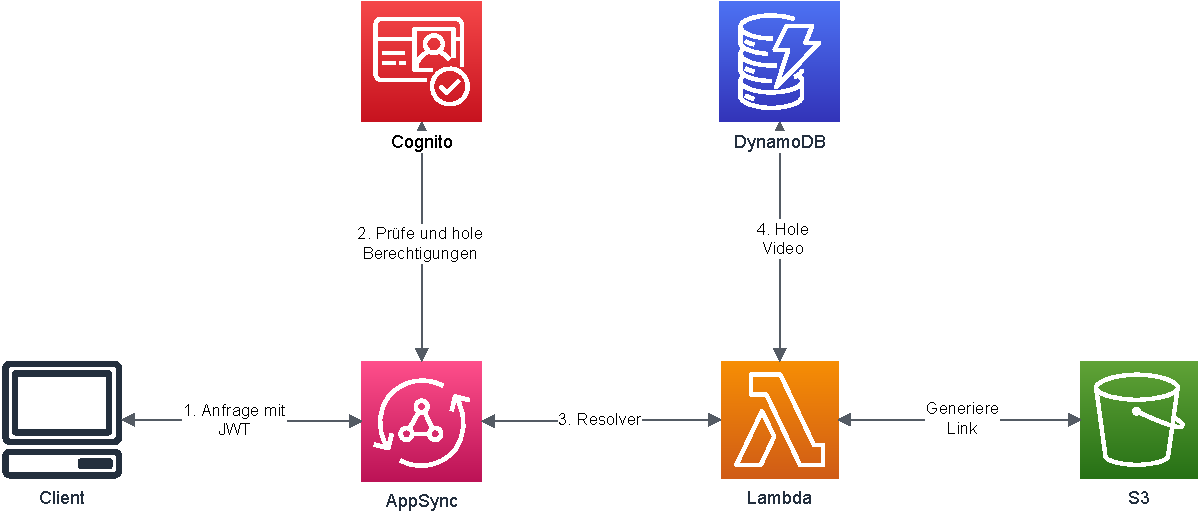
\includegraphics[width=1\columnwidth]{5_aws-amplify/laufzeitsicht_3.pdf}
  \caption{AWS Amplify - Laufzeitsicht - Erstellen von Links}
  \label{Amplify:laufzeitsicht2}
\end{figure}

\subsubsection{Erstellen eines Videos}

\autoref{Amplify:laufzeitsicht3} stellt den Prozess dar, wie ein Video erstellt wird.
\begin{enumerate}
  \item{Zunächst lädt der Nutzer das Video in den S3-Bucket hoch. Die Policy des S3-Buckets verwaltet den korrekten Zugriff auf die Ressource. Die hochgeladene Datei landet in einem privaten Ordner, der außerhalb des Backends ausschließlich für den Besitzer des Objekts aufrufbar ist. Das ist der Nutzer, der das Video hochgeladen hat.}
  \item{Erst dann erstellt der Nutzer eine Anfrage mittels GraphQL und dem JSON Webtoken.}
  \item{AppSync autorisiert den Nutzer und holt die Gruppenzugehörigkeit des Nutzers.}
  \item{Der Resolver führt die verknüpfte Lambda-Funktion aus.}
  \item{Die Funktion kopiert die hochgeladene Datei in einen weiteren Ordner, so dass der Besitzer diese nicht mehr verändern kann. Die hochgeladene Datei im Ursprungsordner wird daraufhin gelöscht.}
  \item{Die Funktion erstellt das Video in der DynamoDB-Tabelle.}
  \item{Die Funktion führt den MediaConvert-Job aus, um das Video mit dem Wasserzeichen zu versehen.}
  \item{Ist die Konvertierung abgeschlossen, benachrichtigt die EventBridge eine weitere Lambda-Funktion, welche das Video dann freischaltet.}
\end{enumerate}

\begin{figure}
  \centering
  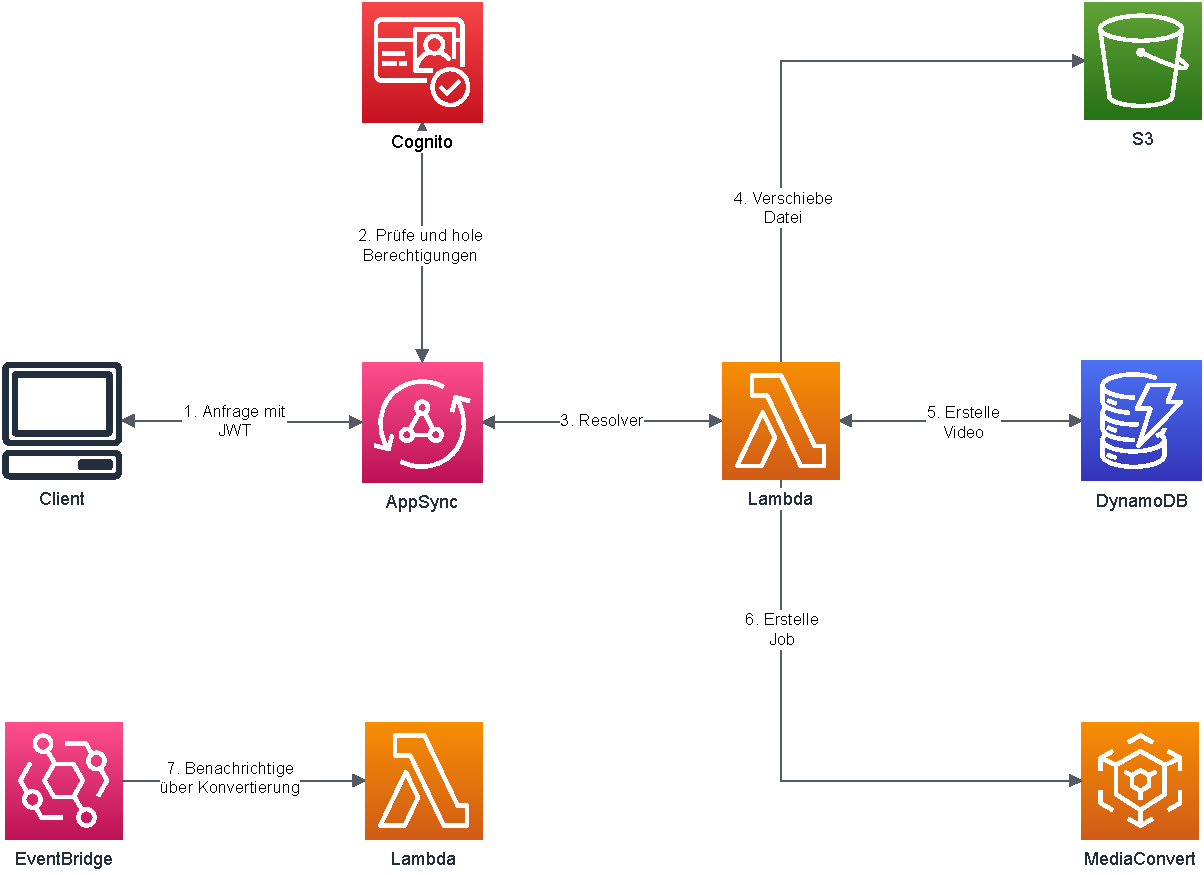
\includegraphics[width=1\columnwidth]{5_aws-amplify/laufzeitsicht_2.pdf}
  \caption{AWS Amplify - Laufzeitsicht - Erstellen eines Videos}
  \label{Amplify:laufzeitsicht3}
\end{figure}

\subsection{Verteilungssicht}

Die Verteilungssicht beschreibt, wie die Bausteine in \ac{AWS} über Stacks verteilt werden. Amplify bündelt die Verteilung des Backends und des Frontends über eine Pipeline. Diesen Sachverhalt stellt \autoref{Amplify:verteilungssicht} dar.

\begin{figure}
  \centering
  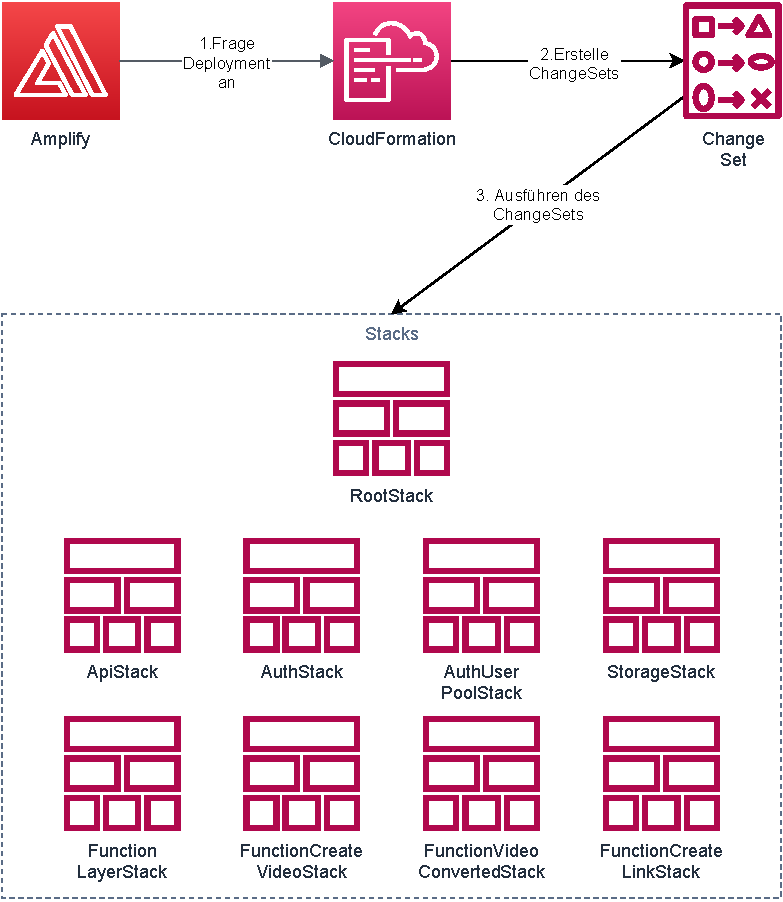
\includegraphics[width=0.75\columnwidth]{5_aws-amplify/verteilungssicht.pdf}
  \caption{AWS Amplify - Verteilungssicht}
  \label{Amplify:verteilungssicht}
\end{figure}

Amplify verteilt das Backend über die CloudFormation mittels Stacks. Außerdem werden nur Stacks und keine NestedStacks genutzt, was die Fehleranalyse vereinfacht. Um eine neue Änderung in das System einzuspielen, erzeugt die CloudFormation ein ChangeSet, welches die Differenz aus dem aktuellen Stand in der Cloud und dem gewünschten Zielzustand ist. Wenn beim Aktualisieren der Stacks ein Fehler auftritt, erfolgt ein Rollback.

Das Frontend wird separat, also nicht über Stacks, verteilt. Dazu nutzt Amplify einen gebündelten Dienst, der über die CloudFront läuft. Letzterer kann allerdings als Black-Box betrachtet werden, da der Entwickler diesen nur durch die Konfiguration beeinflussen kann.

\subsection{Querschnittliche Konzepte und Muster}

Logging
- CloudWatch

Backup
- AWS Backup

- Einbindung über \ac{AWS} Amplify:
  - AWS Elemental MediaConvert als extra Plugin
  - Anpassung an CF-Templates
- Permissions (IAM)

\subsection{Entwurfsentscheidungen}

\subsection{Risiken und technische Schulden}

- Auth: Anpassung, dass statt Identity ID die Pool User Id genutzt wird geht über https://github.com/aws-amplify/amplify-js/issues/54. Leider lässt sich das nicht persistieren, so dass man das bei jedem branch/Projekt neu eintragen muss. Wenn man es im CF-Template ändert, wird die Änderung beim Push rückgängig gemacht. Das ist nicht sehr flexibel. Ggf. Lösung finden und schauen, ob es doch geht.

- CDK als Alternative zu AWS Amplify, da es wesentlich flexibler

\section{Implementierung}

\chapter{AWS Amplify}

Das folgende Kapitel beschreibt die Architektur und die Implementierung mit Amplify.

\section{Architektur}

todo

\subsection{Lösungsstrategie}

Die Architektur folgt dem Aufbau einer Drei"=Schichten"=Architektur:
\begin{itemize}
  \item Präsentationsschicht
    \begin{itemize}
      \item React.js
      \item amplify-js
    \end{itemize}
  \item Logikschicht
    \begin{itemize}
      \item AppSync
      \item Lambda
      \item Cognito
      \item Elemental MediaConvert
      \item EventBridge
      \item IAM
    \end{itemize}
  \item Datenhaltungsschicht
    \begin{itemize}
      \item DynamoDB
      \item S3
      \item Cognito
      \item IAM
      \item AWS Backup
    \end{itemize}
\end{itemize}

Die Dienste Cognito und IAM befindet sich zugleich in zwei Schichten, da dort neben der Logik für Authentifizierung und Autorisierung auch die Benutzer persistiert werden.

Durch die ausschließliche Verwendung interner Dienste von \ac{AWS}, keiner Eigenentwicklungen für die Benutzerverwaltung und den vorgegebenen Technologien sind die Rahmenbedingungen für dieses Projekt nicht missachtet, so dass die beiden Technologien weiterhin vergleichbar sind.

\autoref{Kap2:NFAs} zeigt Lösungsansätze, um die nichtfunktionalen Anforderungen, auch Qualitätsziele genannt, zu erreichen.

\begin{table}[h]
  \caption{Lösungsansatz für nichtfunktionale Anforderungen}
  \label{Kap2:NFAs}
  \renewcommand{\arraystretch}{1.2}
  \centering
  \sffamily
  \begin{footnotesize}
    \begin{tabularx}{0.9\textwidth}{l l X}
      \toprule
      \textbf{Anforderung} & \textbf{Dienst} & \textbf{Ansatz}\\
      \midrule
        \emph{Verfügbarkeit} & Amplify & Amplify bietet für Frontend und Backend ein Zero-Downtime Deployment. \\
        \emph{Skalierbarkeit} & - & Durch die Serverless-Architektur skalieren Dienste automatisch innerhalb der \ac{AWS}-Cloud.\\
        \emph{Analysierbarkeit} & CloudWatch & Durch den Einsatz von CloudWatch können Anfragen für jeden Dienst nachvollzogen werden.\\
        \emph{Interoperabilität} & AppSync & Durch den Einsatz von AppSync ist mit GraphQL eine einheitliche Schnittstelle sichergestellt.\\
        \emph{Backups} & AWS Backup & Durch den Einsatz von AWS Backup werden automatisiert Backups aufgesetzt.\\
        \emph{Wiederherstellbarkeit} & AWS Backup &  Das von AWS Backup erstellte Backup für die Datenbank DynamoDB kann manuell eingespielt werden.\\
      \bottomrule
    \end{tabularx}
  \end{footnotesize}
  \rmfamily
\end{table}

\subsection{Bausteinsicht}

Die Architektur ist unterteilt in Frontend (Präsentationsschicht) und Backend (Logik- und Datenhaltungsschicht). Das Frontend wird nicht näher beschrieben, da Amplify dieses vollständig verwaltet. Das Backend besteht aus Stacks, welche zugleich den Code als auch die Infrastruktur repräsentieren. Diese werden im folgenden Abschnitt dargestellt:
\begin{itemize}
  \item{Der \textit{RootStack} enthält alle darunterliegenden Stacks sowie Ressourcen zum Deployment von Amplify.}

  \item{Der \textit{ApiStack} besteht aus den Diensten AppSync und DynamoDB. AppSync besteht aus einer GraphQLApi, die ein GraphQLSchema enthält. Außerdem nutzt AppSync Resolver, um ein Mapping über VTL zur DynamoDB-Tabelle zu ermöglichen. Um eine Verbindung zu einer Lambda-Funktion zu ermöglichen, existiert auch mindestens eine DataSource.}

  \item{Der \textit{AuthStack} regelt die Authentifizierung und Autorisierung von Benutzern über den Dienst Cognito. Dieser besteht aus einem UserPool und einem IdentityPool und den entsprechenden IAM-Rollen und Policies. Des weiteren besteht der Stack aus einem UserPoolClient, über welchen Anfragen auf Cognito erfolgen können. Amplify definiert auch weitere Lambda-Funktionen, um zusätzliche Logik für die Authentifizierung zu ermöglichen.}

  \item{Der \textit{AuthUserPoolGroupStack} dient zur Verwaltung der zusätzlichen UserPoolGroup für Administratoren.}

  \item{Der \textit{StorageStack} dient zur Speicherung der Videos. Dieser enthält einen S3-Bucket sowie eine dazugehören Policy, welchen es Benutzern ermöglicht, Dateien in eigene Ordner hochzuladen sowie andere Ordner lesen zu dürfen. Die Policy unterscheidet zwischen öffentlichen, geschützten und privaten Geltungsbereichen.}

  \item{Der \textit{FunctionLayerStack} bündelt die Node.js-Module als Lambda-Layer, den die weiteren Lambda-Funktionen nutzen.}

  \item{Der \textit{FunctionCreateVideoStack} übernimmt die Erstellung eines Videos in Form einer Lambda-Funktion. Außerdem erstellt der Stack in MediaConvert ein JobTemplate und eine Queue. Des Weiteren definiert der Stack die nötige Policy und Rolle, um der Lambda-Funktion die Zugriffe auf andere Dienste zu ermöglichen.}

  \item{Der \textit{FunctionVideoConvertedStack} besteht aus einer EventBridge-Regel, die bei einer Konvertierung eines Videos aufgerufen wird. Außerdem wird eine Lambda-Funktion mit der nötigen Policy und Rolle erstellt.}

  \item{Der \textit{FunctionCreateLinkStack} besteht aus einer Lambda-Funktion und der nötigen Rolle und Policy, um einen signierten zeitlich begrenzt gültigen Video-Link zu erstellen.}
\end{itemize}

Die Stacks \textit{RootStack}, \textit{ApiStack}, \textit{AuthStack}, \textit{AuthUserPoolGroupStack} und \textit{StorageStack} erstellt Amplify selbst. Die restlichen Stacks sind selbst erstellte bzw. angepasste Plugins, da die Dienste nicht vollständig in Amplify vorhanden sind.

\subsection{Laufzeitsicht}

Die Laufzeitsicht beschreibt die wichtigsten Prozesse und wie die Bausteine miteinander interagieren.

\subsubsection{Lesen, Aktualisieren und Löschen eines Videos}

\begin{figure}
  \centering
  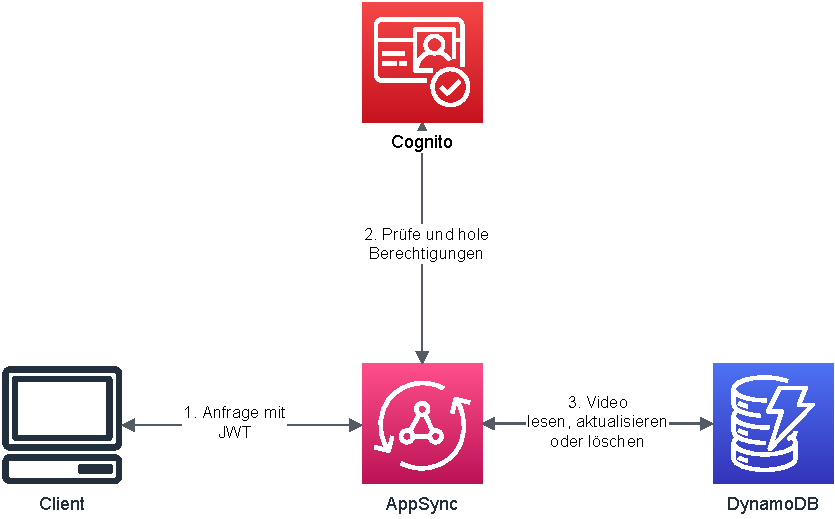
\includegraphics[width=0.75\columnwidth]{5_aws-amplify/laufzeitsicht_1.pdf}
  \caption{AWS Amplify - Laufzeitsicht - Lesen, Aktualisieren und Löschen eines Videos}
  \label{Amplify:laufzeitsicht1}
\end{figure}

\autoref{Amplify:laufzeitsicht1} stellt den Prozess dar, wie Videos von Nutzern gelesen, aktualisiert oder gelöscht werden. Dieser wird im folgenden Abschnitt näher erläutert:
\begin{enumerate}
  \item{Der Nutzer stellt eine Anfrage mittels GraphQL und dem JSON Webtoken.}
  \item{AppSync autorisiert den Nutzer und holt die Gruppenzugehörigkeit des Nutzers.}
  \item{Der Resolver leitet die Anfrage unter Berücksichtigung der Gruppenzugehörigkeit des Nutzers an DynamoDB weiter. Die nötigen Datenbankoperationen werden über DynamoDB ausgeführt.}
\end{enumerate}

Zusätzlich dazu müssen signierte temporäre Links erstellt werden, um die Sicherheit zu gewährleisten. Dieser Ablauf, der in \autoref{Amplify:laufzeitsicht2} dargestellt wird, enthält noch eine zusätzlich Abfrage auf S3, um den Link zu erstellen.

\begin{figure}
  \centering
  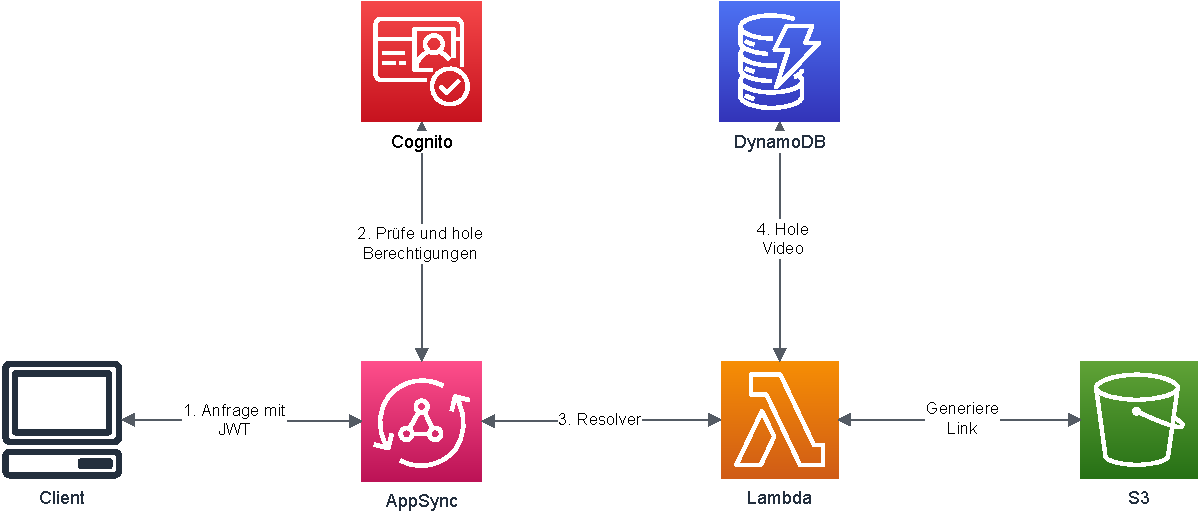
\includegraphics[width=1\columnwidth]{5_aws-amplify/laufzeitsicht_3.pdf}
  \caption{AWS Amplify - Laufzeitsicht - Erstellen von Links}
  \label{Amplify:laufzeitsicht2}
\end{figure}

\subsubsection{Erstellen eines Videos}

\autoref{Amplify:laufzeitsicht3} stellt den Prozess dar, wie ein Video erstellt wird.
\begin{enumerate}
  \item{Zunächst lädt der Nutzer das Video in den S3-Bucket hoch. Die Policy des S3-Buckets verwaltet den korrekten Zugriff auf die Ressource. Die hochgeladene Datei landet in einem privaten Ordner, der außerhalb des Backends ausschließlich für den Besitzer des Objekts aufrufbar ist. Das ist der Nutzer, der das Video hochgeladen hat.}
  \item{Erst dann erstellt der Nutzer eine Anfrage mittels GraphQL und dem JSON Webtoken.}
  \item{AppSync autorisiert den Nutzer und holt die Gruppenzugehörigkeit des Nutzers.}
  \item{Der Resolver führt die verknüpfte Lambda-Funktion aus.}
  \item{Die Funktion kopiert die hochgeladene Datei in einen weiteren Ordner, so dass der Besitzer diese nicht mehr verändern kann. Die hochgeladene Datei im Ursprungsordner wird daraufhin gelöscht.}
  \item{Die Funktion erstellt das Video in der DynamoDB-Tabelle.}
  \item{Die Funktion führt den MediaConvert-Job aus, um das Video mit dem Wasserzeichen zu versehen.}
  \item{Ist die Konvertierung abgeschlossen, benachrichtigt die EventBridge eine weitere Lambda-Funktion, welche das Video dann freischaltet.}
\end{enumerate}

\begin{figure}
  \centering
  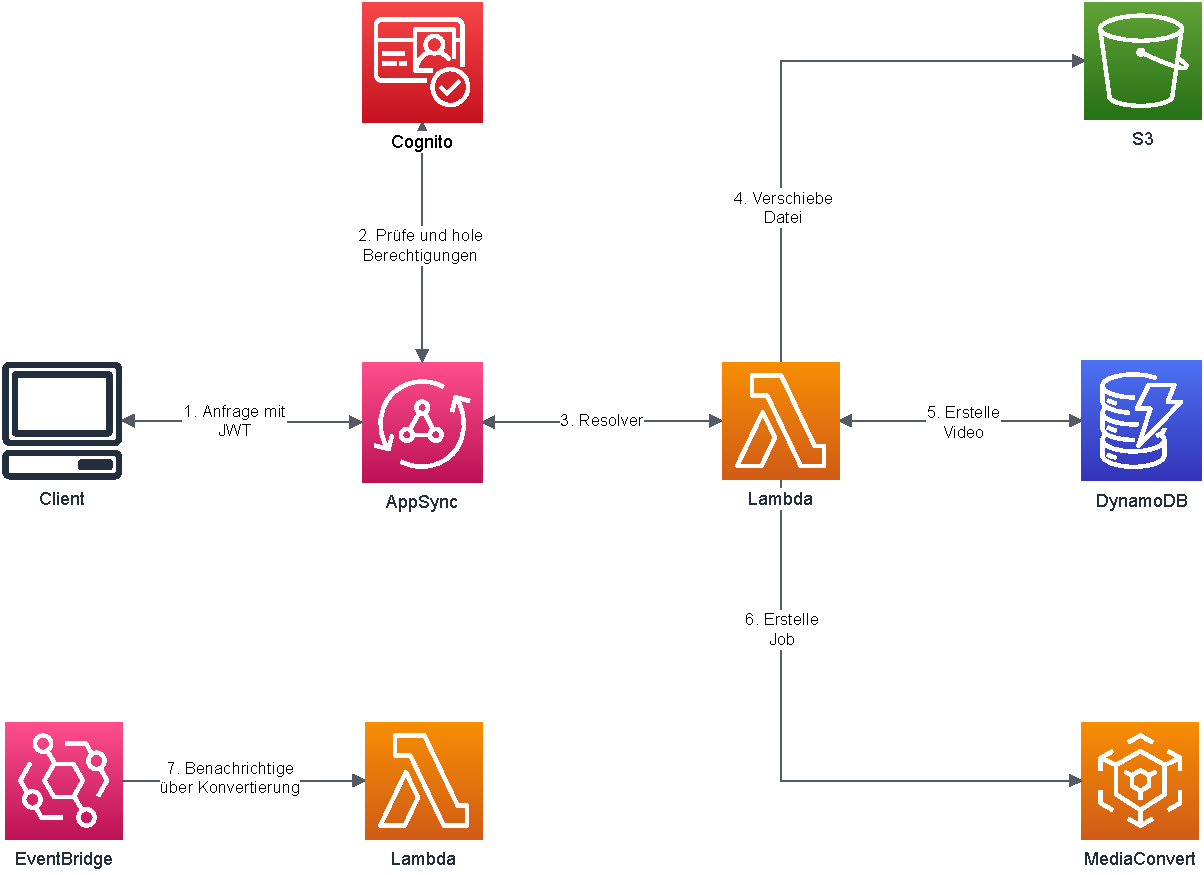
\includegraphics[width=1\columnwidth]{5_aws-amplify/laufzeitsicht_2.pdf}
  \caption{AWS Amplify - Laufzeitsicht - Erstellen eines Videos}
  \label{Amplify:laufzeitsicht3}
\end{figure}

\subsection{Verteilungssicht}

Die Verteilungssicht beschreibt, wie die Bausteine in \ac{AWS} über Stacks verteilt werden. Amplify bündelt die Verteilung des Backends und des Frontends über eine Pipeline. Diesen Sachverhalt stellt \autoref{Amplify:verteilungssicht} dar.

\begin{figure}
  \centering
  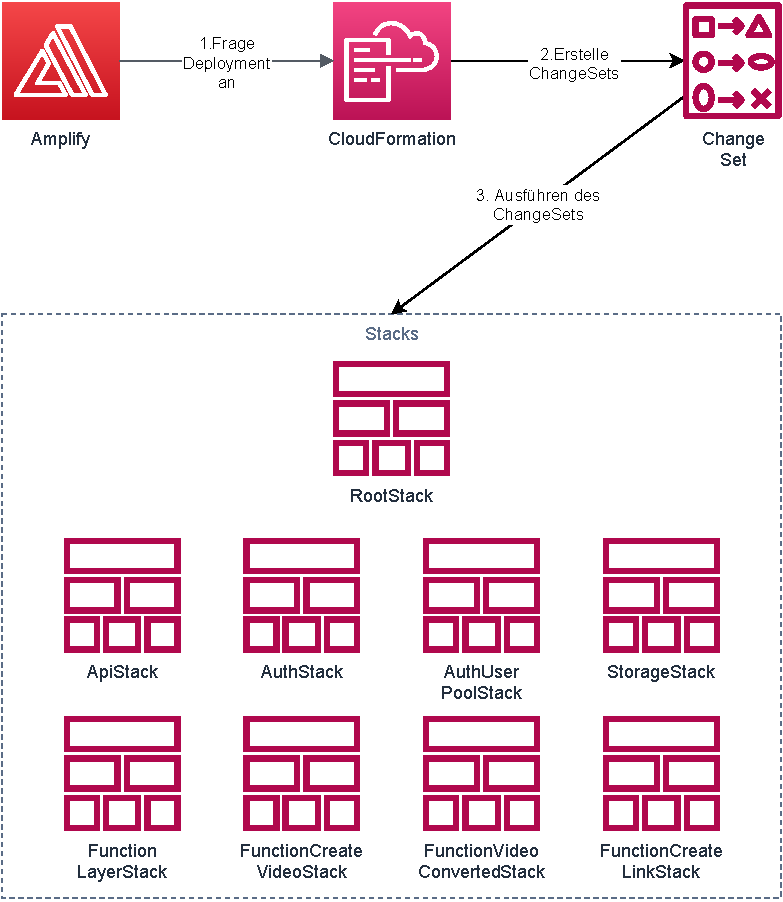
\includegraphics[width=0.75\columnwidth]{5_aws-amplify/verteilungssicht.pdf}
  \caption{AWS Amplify - Verteilungssicht}
  \label{Amplify:verteilungssicht}
\end{figure}

Amplify verteilt das Backend über die CloudFormation mittels Stacks. Außerdem werden nur Stacks und keine NestedStacks genutzt, was die Fehleranalyse vereinfacht. Um eine neue Änderung in das System einzuspielen, erzeugt die CloudFormation ein ChangeSet, welches die Differenz aus dem aktuellen Stand in der Cloud und dem gewünschten Zielzustand ist. Wenn beim Aktualisieren der Stacks ein Fehler auftritt, erfolgt ein Rollback.

Das Frontend wird separat, also nicht über Stacks, verteilt. Dazu nutzt Amplify einen gebündelten Dienst, der über die CloudFront läuft. Letzterer kann allerdings als Black-Box betrachtet werden, da der Entwickler diesen nur durch die Konfiguration beeinflussen kann.

\subsection{Querschnittliche Konzepte und Muster}

Logging
- CloudWatch

Backup
- AWS Backup

- Einbindung über \ac{AWS} Amplify:
  - AWS Elemental MediaConvert als extra Plugin
  - Anpassung an CF-Templates
- Permissions (IAM)

\subsection{Entwurfsentscheidungen}

\subsection{Risiken und technische Schulden}

- Auth: Anpassung, dass statt Identity ID die Pool User Id genutzt wird geht über https://github.com/aws-amplify/amplify-js/issues/54. Leider lässt sich das nicht persistieren, so dass man das bei jedem branch/Projekt neu eintragen muss. Wenn man es im CF-Template ändert, wird die Änderung beim Push rückgängig gemacht. Das ist nicht sehr flexibel. Ggf. Lösung finden und schauen, ob es doch geht.

- CDK als Alternative zu AWS Amplify, da es wesentlich flexibler

\section{Implementierung}

\label{lastpage}

\cleardoublepage

\singlespacing

\pagenumbering{roman}
\setcounter{page}{\value{frontmatterpage}}

\addchap{\hsmaabbreviations}
% Die längste Abkürzung kann in die eckigen Klammern
% bei \begin{acronym} geschrieben, um einen hässlichen
% Umbruch zu verhindern
%
% ACHTUNG: Sie müssen die Abkürzungen von Hand alphabetisch
%          sortieren. Das passiert nicht automatisch.
\begin{acronym}[UUID]
\acro{EC2}{Elastic Compute Cloud}
\acro{API}{Application Interface}
\acro{AWS}{Amazon Webservices}
\acro{UUID}{Universally Unique Identifier}
\acro{IaaS}{Infrastructure as a Service}
\acro{PaaS}{Platform as a Service}
\acro{FaaS}{Function as a Service}
\acro{SaaS}{Software as a Service}
\acro{BaaS}{Backend as a Service}
\acro{MBaaS}{Mobile Backend as a Service}
\acro{STaaS}{Storage as a Service}
\end{acronym}

\cleardoublepage
\phantomsection
\addcontentsline{toc}{chapter}{\hsmalistoftables}
\listoftables

\cleardoublepage
\phantomsection
\addcontentsline{toc}{chapter}{\hsmalistoffigures}
\listoffigures

\cleardoublepage
\phantomsection
\addcontentsline{toc}{chapter}{\hsmalistings}
\lstlistoflistings

\begingroup
\cleardoublepage
\begin{flushleft}
\let\clearpage\relax
\printbibliography
\end{flushleft}
\endgroup

\end{document}